%Started on Wednesday, 9th August 2006
%Aug: 11, 22, 23, 30
%Sep:  7
% 2007
%Jan: 15, 16, 22
%Feb:  4,  5
%Mar: 12, 20, 21, 27, 30, 31
%Apr:  3
%May: 12, 14

\documentclass[phd,leftchapter]{msthesis}

%
% Packages
%
\usepackage{amsmath}  % for \text, \binom
\usepackage{amsthm}   % for proof
\usepackage{amssymb}  % for \mathbb (from amsfonts, which is included by this}
\usepackage{verbatim,enumerate}
\usepackage{longtable,graphicx}
\usepackage[chapter]{algorithm}
\usepackage{algorithmic}

%\usepackage[notref,notcite]{showkeys}


%
% Macros
%
%
% Item point
%
\renewcommand{\labelitemi}{$\circ$}

%
% Framed box
%
\addtolength{\fboxsep}{0.5ex}
\newcommand{\fb}[1]{
 \begin{center}
    \fbox{\parbox{.9\textwidth}{#1}}
 \end{center}
}

%
% Bounded text
%
\newcommand{\bt}[1]{
\noindent\hrulefill
\vspace{-2\parsep} {#1} \vspace{-2\parsep}
\noindent\hrulefill
}

%
% Set of real numbers
%
\newcommand{\R}{\mathbb{R}}

%
% Big-O
%
\newcommand{\bigO}{\mathcal{O}}

%
% Equations
%
\newcommand{\be}{\begin{equation}}
\newcommand{\ee}{\end{equation}}

%
% Difficult names
%
\newcommand{\yildirim}{Y{\i}ld{\i}r{\i}m\ }

%
% Theorems
%
\newtheorem{prop}[subsection]{Proposition}
\newtheorem{thm}[subsection]{Theorem}
\newtheorem*{thm*}{Theorem}
\newtheorem{lemma}[subsection]{Lemma}
\newtheorem*{lemma*}{Lemma}
\newtheorem{cor}[subsection]{Corollary}
\newtheorem{claim}[subsection]{Claim}
\newtheorem{condition}[subsection]{Condition}
\newtheorem{conjecture}[subsection]{Conjecture}
\theoremstyle{definition}
\newtheorem{defn}[subsection]{Definition}
\newtheorem*{defn*}{Definition}
\newtheorem{exm}[subsection]{Example}
\newtheorem{exms}[subsection]{Examples}
\newtheorem{notelabel}[subsection]{Note}
\newtheorem{note}[subsection]{Note}
\newtheorem{question}[subsection]{Question}
\newtheorem*{question*}{Question}

%
% Multiline comments
%
\newcommand{\ignore}[1]{}


\frenchspacing

\title{Advances in Interior Point Methods \\
       for Large-Scale Linear Programming}
\author{Marco Colombo}
\submityear{2007}


%
% Begin document
%
\begin{document}

\maketitle

\dedication{
            Se'n foi me de chesta br\"ogna ch\'e? \\
\vspace{3em}
            If nothing else it true, well this is \\
	    If nothing else meant anything \\
	    the silence ended and I forgot, I forgot, I forgot. \\
\vspace{3em}
            I wish that I could find it, I wish I'd let it go \\
	    I wish my arms could hold it, will I ever know? \\
	    It may or may not happen\dots
}
\standarddeclaration

%
% Abstract
%
\begin{abstract}
  %Started on Wednesday, 9th August 2006
% 2007
%Feb: 12

%
% Abstract
%

This research studies two implementable techniques that improve
the practical performance of existing computational implementations 
of interior point methods for linear programming.
Also, it provides the analysis of the concept of symmetric neighbourhood 
as the driving tool for the analysis and understanding of the good 
performance of some practical algorithms. 

The use of the symmetric neighbourhood and the recent
theoretical understanding of the behaviour of Mehrotra's
corrector direction motivate the introduction of a weighting
mechanism that can be applied to any corrector direction,
whether originating from Mehrotra's predictor--corrector algorithm
or as part of the multiple centrality correctors technique.
Such modification on the way a corrector direction is applied
concentrates on ensuring that such a direction can positively
contribute to a successful iteration by increasing the overall
stepsize. Also, it tries to use the information from a corrector
direction even when otherwise it would be rejected because it
produces a short stepsize. 
The usefulness of the weighting strategy is documented through
a complete numerical experience on various sets of publicly
available test problems.

The second advance is the development of an efficient way of 
constructing a starting point for structured large-scale 
stochastic linear programs.
We generate a computationally viable warmstart point by solving 
to low accuracy a stochastic problem of much smaller dimension.
The solution to the reduced problem is then expanded to the
size of the problem instance, and used to initialise the
interior point algorithm.
The performance of this warm-start strategy is verified through 
a series of tests on problem instances coming from various stochastic
programming sources.

\end{abstract}

%
% Acknowledgements
%
\begin{acknowledgements}
  %Started on Wednesday, 9th August 2006
%Aug: 11
% 2007
%Jan: 15, 17
%May: 12, 13

%
% Acknowledgements
%

I would like to thank Prof.~Jacek Gondzio for proposing such an
interesting and challenging project. 
He shared his enthusiasm for interior point methods, and 
instilled in me a very keen interest in pursuing a research in this field.
Moreover, his dedicated support and the frequent discussions
have been crucial to my successful
completion of this research.

Dr.~Andreas Grothey's contribution to the success of this research
cannot be underestimated. 
He has had the patience of introducing me to \OOPS, and helped me out
in the frequent occasions of panic.

Big thanks to Cathy: she has offered to proofread this thesis, and she
has done a great job. 

Many friends deserve to be mentioned here as well, for the time spent together,
the conversations, and the help that I received in many forms from them.
So thanks to Aghlab, Gaurav, Iria, and to those that have left from Edinburgh
like Paulo, Eleni and Giorgos. 
I am particularly indebted to Andrea, who has been close to me through
most of this time, and has experienced the ups and downs of my PhD life.
It's been very nice to share room 6320 with Cathy, David, Elingborg, Rosemary
and Tomas. They have been great office mates and
friends too!

I got lots of support from my family, in particular in the last few months.
It's been really nice feeling cheered and spurred by them!

\end{acknowledgements}

%
% Table of contents
%
\tableofcontents

%
% Chapters
%
\chapter{Background and introduction.}
%Started on 30th August 2006
%Aug: 31
%Sep:  1,  8

%
% Chapter: Background and introduction.
%
\label{ch:Introduction}

In this chapter we present the background and motivations for
this research.

%
% Section
%
\section{Linear programming}

\fb{
An historical account of linear programming is given in \cite{Schrijver86}.
}

\fb{
The simplex method as an active set method.
}

\fb{
Maybe something on the difficulty of LP? And something that motivates
the fact that a solution has to be at a vertex.
}

The simplex method reaches a solution by visiting a sequence of 
vertices of the polyhedron, moving from one vertex to an adjacent 
one characterized by a better objective function value. The polyhedron 
corresponding to a linear system of $m$ constraints in $n$ variables 
($m < n$) has a number of vertices equal to
\[
\binom{n}{m} = \frac{n!}{m!(n-m)!}.
\]

\fb{
Klee and Minty's example of bad behaviour of the simplex method
(when Dantzig's pivoting rule is used).
}

In real-life problems, this situation never arises, and not all of 
these vertices will have to be visited. Besides, given the monotonic
way of choosing the next vertex, in the non-degenerate case the set 
of possible vertices decreases after each iteration. Degeneracy
complicates things because at a degenerate vertex, the simplex method
may try different changes of basis without actually moving away
from the vertex.

\fb{
Discussion on the complexity of linear programming. How the simplex
method is exponential.
}

\fb{
The search for a polynomial algorithm and the ellipsoid method.

In Khachiyan's ellipsoid method, the polyhedron is inscribed in a sequence
of ellipsoids of decreasing size. If the problem has a solution, the 
centers of these ellipsoids converge to the optimal solution; otherwise,
their size decreases to zero.

The ellipsoid method finds a solution in $\bigO(n^2L)$ iterations,
thus has polynomial complexity. Since this worst-case bound
is generally attained, its practical performance is not competitive
with other solution methods. Besides, other problems relate to round-off
errors and dense matrix computation.

However, the ellipsoid method is often used in the contex of
combinatorial optimization as an analytic tool to prove complexity
results for algorithms.
}

We know polynomial-time algorithms for linear programming, 
namely the ellipsoid method (see \cite[ch.~13]{Schrijver86} 
and \cite[ch.~I.6]{ip:NemhauserWolsey88}) and interior point 
methods (\cite{ipm:Wright97}). Despite being an exponential 
algorithm, the simplex method shows polynomial complexity in 
the average time, and is therefore widely adopted in the 
solution of linear programming problems.


%
% Section
%
\section{Interior point methods}

Since their introduction following Karmarkar's groundbreaking paper
\cite{Karmarkar}, interior point methods (IPMs for short) have attracted 
the interest of a growing number of researchers.

\fb{
Karmarkar's algorithm is a primal algorithm based on a projection
in some transformed space and steepest descent. It uses a potential
function to measure the progress. It has $\bigO(nL)$ complexity.

}

Over the last 20 years, an impressive wealth of theoretical research
has been published, and computational developments have brought life
to a field, that of Linear Programming, that seemed not to attract much
attention anymore.

\fb{
Cite the reports on how much the simplex method has improved as a 
consequence of that.
}

Interior point methods are well-suited to solving very
large scale optimization problems. Their theory is well understood
\cite{ipm:Wright97} and the techniques used in their implementation 
are documented in extensive literature (see, for example, 
\cite{AndersenGondzioMeszarosXu,GondzioTerlaky} and the references therein).

\fb{
Cases where the simplex method cannot be beaten: hyper-sparsity.
}

\fb{
Contrary to active set algorithms, interior point methods reach a
solution only asymptotically. Mention crossover strategies and finite
termination.
Once a solution with a prescribed optimality tolerance has been found,
such a point can be projected upon a face of the polyhedron.
}

%
% Section
%
\section{Other stuff}

A generic optimization algorithm can be summarised in the following
scheme:

\bt{
\begin{description}
\item[Given] an initial iterate;
\item[Repeat] for $k=0,1,2,\ldots$ 
  \begin{itemize}
  \item Determine a search direction.

  \item Determine how far to move along it.

  \item Move to the next point.
  \end{itemize}

\item[Until] some termination criteria are met.
\end{description}
}

Each of the point of this simplified algorithm has to be specialised
to the specific algorithm we are talking about.

%
% Section
%
\section{Motivation of this thesis}

Optimization algorithms are extremely important in real-life 
applications. Theoretical advances are necessary for the 
understanding of the current state and the opening of new avenues 
of research. 

However, theory per se has rarely a direct impact on the lives 
of those who use optimization as a tool to solver their problems.
It is therefore necessary that the understanding gathered from
theoretical studies is then transformed into actual practical
tools. This often requires the implementation of computer programs.

The process of creating computationally efficient methods from
theoretical studies is not as direct as it might sound. It usually
involves relaxing many of the theoretical assumptions, and ensuring
other properties.

Therefore we will put great effort in accompanying theoretical
results with the corresponding computational considerations. While
in a few cases these can be treated simultaneously, generally that
will not be possible. There are a few reasons for this:
\begin{itemize}
\item Theoretical assumptions may not be realistic: this is the case
when a condition stated in a theorem is not realistically satisfiable 
in practice (for examples, bounds on some quantities). 
\item Theoretical assumptions may be too restrictive: this happens
when the theory predicts a certain behaviour under some conditions
but actually in practice it happens anyway, or provides a worst-case 
result which may be far from the average one.
\item Theoretical requirement is computationally expensive: this 
may happen when the satisfaction of a certain condition is not 
computationally viable, and workarounds are usually employed.
\end{itemize}

Besides this, the practical implementation of an algorithm happens
in a context that is not amenable to theoretical analysis for the
following reasons:
\begin{itemize}
\item Finite precision of floating-point arithmetic;
\item Heuristic choices;
\item 
\end{itemize}

%
%
\section{Main references}

The original results presented in this thesis are mainly based on two
papers that have been submitted for publication.

The first \cite{ColomboGondzio05} is a joint work with Jacek Gondzio.
The main objective of this paper was to analyze the efficiency of
corrector directions in the light of the theoretical studies of Cartis
\cite{Cartis04,Cartis05}. It concentrates on ensuring that a corrector
direction computed at the current iterate is not rejected because it
produces a short stepsize. Such a behaviour usually is manifested when
the point is badly centered or highly infeasible.

The second \cite{ColomboGondzioGrothey06} is a joint work with
Jacek Gondzio and Andreas Grothey. It aims at developing an
efficient way of constructing a starting point for structured 
large-scale stochastic linear programs.


\chapter[Interior point methods for linear programming.]{Interior point methods \\ for linear programming.}
%Started on 9th August 2006
%Aug: 11, 22, 23, 24, 25, 28, 29, 30, 31
%Sep:  1,  7,  8
%Jan 2007: 15, 16, 17

%
% Chapter: Interior point methods
%
\label{ch:Ipm}

Interior point methods are well-suited to solving very
large scale optimization problems. Their theory is well understood
\cite{ipm:Wright97} and the techniques used in their implementation are
documented in extensive literature (see, for example, 
\cite{AndersenGondzioMeszarosXu,GondzioTerlaky} and the references therein).

This chapter is devoted to the derivation and analysis of interior 
point methods. 
The theoretical developments presented will be accompanied by computational 
arguments.


%
% Section
%
\section{Primal--dual path-following methods}
\label{sec:Derivation}

Consider the following primal--dual pair of linear programming problems 
in standard form
%
\begin{eqnarray} \label{eq:PrimalDualPair}
  \begin{array}{rlp{2cm}rl}
%   \mbox{\small Primal } & & & \mbox{\small Dual } \\[0.1cm]
    \mbox{ min }  & c^T x  & & \mbox{ max }  & b^T y \\
    \mbox{ s.t. } & Ax = b,& & \mbox{ s.t. } & A^T y + s = c, \\
                  & x \geq 0; &  &   & y \mbox{ free,} \;\; s \geq 0,
  \end{array}
\end{eqnarray}
%
where $A \in \R^{m \times n}$, $x, s, c \in \R^{n}$ 
and $y, b \in \R^{m}$. We assume, without loss of generality,
that $A$ has full row rank, as linearly dependent rows can be
removed without changing the solution set.
This also implies that a feasible $s \ge 0$ determines in a unique
way the value of $y$.

We recall here some well-known results on the relationship between
problems $\mathcal{P}$ and $\mathcal{D}$ in linear programming. 
These can be found in plenty of sources, for example \cite{lp:Chvatal} \ldots

\fb{
Find these sources!
}

We define the set of primal feasible points
\be \label{eq:PrimalFeasibleSet}
\mathcal{F} = \{ x : Ax = b, \; x \ge 0 \},
\ee
and equivalently the set of dual feasible points
\be \label{eq:DualFeasibleSet}
\mathcal{D} = \{ (y,s) : A^T y + s = c, \; s \ge 0 \}.
\ee

The primal--dual pair (\ref{eq:PrimalDualPair}) can therefore be written as
\be \label{eq:PrimalDualPair2}
\min \; c^T x \quad x \in \mathcal{F}, \qquad
\min \; b^T y \quad (y,s) \in \mathcal{D},
\ee

Problem P has a solution iff $\mathcal{F} \ne \emptyset$;
if also $\mathcal{D} \ne \emptyset$, then both problems admit an
optimal solution $(x^*, y^*, s^*)$, and the objective function 
values of both problems at that point coincide (strong duality).

However, one of the sets might be empty: in such a case, an optimal
solution for problem (\ref{eq:PrimalDualPair2}) does not exist,
as the set is either unbounded or empty as well.

\fb{
Formalize these results.
}

\fb{
Introduce barrier problems and show similar theorems for them,
as done in Megiddo \cite{Megiddo}.
}

The Karush-Kuhn-Tucker (KKT) conditions express first-order optimality 
conditions for the primal--dual pair (\ref{eq:PrimalDualPair}).
They can be expressed as
\be  \label{eq:KKT}
\begin{array}{rcl}
  Ax      &=& b \\
  A^Ty +s &=& c \\
  XSe     &=& 0 \\
  (x,s)   &\ge& 0,
\end{array}
\ee
where $X, S \in \R^n$ are diagonal matrices with elements 
$x_i$ and $s_i$ respectively, and $e \in \R^n$ is a vector 
of ones. In other words, an optimal solution is characterised by 
primal feasibility, dual feasibility and complementarity.

\fb{
Spend a few words on the concept of complementarity.
}

Interior point methods arrive to a solution that satisfies the KKT
conditions (\ref{eq:KKT}) by ``relaxing'' the complementarity constraints.
%
Path-following interior point methods \cite{ipm:Wright97} perturb 
the above conditions by asking the complementarity pairs to align 
to a specific barrier parameter $\mu > 0$,
\[
XSe = \mu e,
\]
while enforcing $(x,s)>0$.

\fb{
The above inequality cannot be strictly enforced, as it would not make
the solution of the KKT conditions (\ref{eq:KKT}) any easier. Instead,
the concept of neighbourhood is required, and is presented in
Section~(\ref{sec:Neighbourhoods}).
}

As $\mu$ is monotonically decreased at each iteration, the solution of the 
perturbed Karush-Kuhn-Tucker conditions approximates better and better
the system of optimality conditions (\ref{eq:KKT}).

If the perturbed KKT system has a solution for any $\mu > 0$, then
it traces a unique continuous path $(x(\mu),s(\mu))$ toward the 
optimal set as $\mu \to 0$. 
In interior-point terminology, such a path is called
the {\em central path}.

%
%
\subsection{The central path}

\fb{
Find out who started the study of the notion of central path. Gonzaga 
\cite{Gonzaga92} says it was Bayer and Lagarias as well as Megiddo.
}

The study of the primal--dual properties of the central path 
was started by Megiddo's seminal paper \cite{Megiddo}, which is 
still considered a basic reference in the interior-point literature.

Many algorithms used in mathematical programming can be interpreted 
as path-following. What is studied here is the path described by the 
barrier functions in linear programming.
The presentation follows the clear and systematic approach of Megiddo
\cite{Megiddo}.

Given a linear program in standard form $P$:
\[
\begin{array}{rl}
  \max        & c^Tx \\
  \mbox{s.t.} & Ax = b, \; x \ge 0,
\end{array}
\]
it is possible to write the corresponding barrier problem $P_\mu$:
\[
\begin{array}{rl}
  \max        & c^Tx + \mu \sum_j \ln x_j \\
  \mbox{s.t.} & Ax = b, \; x > 0.
\end{array}
\]

This second problem is parametrized by the quantity $\mu > 0$, 
tipically small. The presence of the logarithmic barrier forces the iterates 
to stay in the interior of the feasible region. Such approach is 
viable only if it is actually possible to find a point that 
satisfies the constraints.
Note that the objective function is a strictly convex function. 
Therefore, for a fixed $\mu$, the problem has at most one global minimum. 
This global minimum, if it exists, is completely characterized 
by the KKT conditions.

The KKT conditions associated with problem $P_\mu$ are:
\[
\begin{array}{lcc}
  \mu X^{-1}e -A^Ty & = & -c \\
   Ax               & = &  b
\end{array}
\]

If the feasible domain $\{ x: Ax=b,\: x\ge 0 \}$ is bounded, 
then both $P$ and $P_\mu$ have optimal solution. Since the 
objective function in $P_\mu$ is strictly concave, $P_\mu$ 
has a unique solution for every $\mu>0$.

Megiddo then proves the following proposition: problem $P_\mu$ 
is either unbounded for every  $\mu>0$ or has a unique optimal 
solution for every $\mu>0$.

If the KKT system has a solution for any $\mu>0$, then it 
determines a unique continuous path $x(\mu)$ as $\mu\to 0$. 
Moreover, if $A$ has full rank, then the value of $y$ is 
uniquely determined by the value of $x$. Therefore, the KKT 
system has a unique solution $(x(\mu),y(\mu))$.

Megiddo shows that $c^Tx(\mu)\to c^Tx^*$ as $\mu\to 0$. 
Furthermore, he proves the stronger result that 
$x(\mu)\to x^*$ as $\mu\to 0$.

\fb{
\begin{itemize}
\item Properties of the curvature of the central path \cite{VavasisYe}, 
and straight line towards the end \cite{Megiddo}.
\item Explore the ``videos'' of the central path on Wright's webpage.
\item Problems with central path defined as analytic center: Terlaky's
 Klee-Minty example, discussion with Coralia (she mentioned a 
chapter in Ye's book).
\end{itemize}
}

\fb{
Gonzaga \cite{Gonzaga92} mentions various centers (center of gravity, 
analytic center). See also Nick Gould's slides at cerfacs.
}

\fb{
In \cite[Section 8]{Gonzaga92} there is a nice part on scaling,
and also on primal--dual scaling.
}

\fb{
Show the change of variables $s = \mu X^{-1}e$, otherwise $s$ seems
to appear magically in the following section.
}

\fb{
Mehrotra notices that ``it is not clear if the central path (with
equal weights) is the best path to follow, particularly since it
is affected by the presence of redundant constraints. Furthermore,
the points on (or near) the central path are only intermediate to
solving the linear programming problem. It is only the limit point 
on this path that is of interest to us.''
}

%
%
\subsection{Neighbourhoods}
\label{sec:Neighbourhoods}

Two neighbourhoods are often used in theoretical developments.

The first is based on the Euclidean norm, and it is often referred
to as the {\em tight neighbourhood}:
\[
\mathcal{N}_2(\theta) = \{ (x,y,s) \in \mathcal{F}^0 :
                         \| XSe - \mu e \|_2 \le \theta\mu \}.
\]
This neighbourhood follows very closely the central path:
search directions generated from points in this neighbourhood can be 
followed with full step, and the barrier parameter can be decreased
by a small amount at each iteration (giving rise to the name
of {\em short-step algorithms} to the algorithms that are based on
this neighbourhood). 
The closeness to the central path that the tight neighbourhood
imposes and maintains allows to produce the best convergence result
for linear programming. 
However, since the reduction in the barrier parameter at each iteration 
is very small, the practical value of short-step algorithms is small.

The other commonly used neighbourhood is instead based on the infinity norm, 
and it is often called {\em wide neighbourhood}:
\[
\mathcal{N}_{-\infty}(\gamma) = \{ (x,y,s) \in \mathcal{F}^0 :
                         x_is_i \ge \gamma\mu, \; \forall i \}.
\]
Algorithms based on such a neighbourhood are allowed to generate
iterates that follow more loosely the central path. The iterates 
have more freedom of movement as they can approach the border.
Also, algorithms based on the wide neighbourhood (usually denoted as
{\em long-step algorithms}) are less conservative and can decrease 
the barrier parameter more rapidly.
However, the Newton direction computed from points in the wide 
neighbourhood  has weaker properties, and a linesearch procedure is
needed to ensure that the positivity of the $(x,s)$ iterates is
preserved.

In Section (\ref{sec:SymNeighbourhood}) we will study a variation
of the $\mathcal{N}_{-\infty}$ neighbourhood which better describes
the centrality requirements needed for a practical algorithm.

\fb{
Describe the analytic center and its properties.
}


%
%
\subsection{Solving the perturbed KKT conditions}

Path-following interior point methods seek a solution 
to the system of equations
\[
F(x,y,s) = \left[
  \begin{array}{c}
    Ax-b \\
    A^Ty+s-c \\
    XSe - \mu e \\
  \end{array} \right] = 0,
\]
which is nonlinear in the perturbed complementarity constraints.
We use Newton's method to linearise the system according to
\[
\nabla F(x,y,s) \Delta(x,y,s) = -F(x,y,s),
\]
and obtain the so-called step equations
%
\be \label{eq:NewtonSystem}
\left[ \begin{array}{ccc}
    A & 0 & 0 \\ 0 & A^T & I \\ S & 0 & X
  \end{array} \right]
\left[ \begin{array}{c}
    \Delta x \\  \Delta y \\  \Delta s
  \end{array} \right] =
\left[ \begin{array}{c}
    b - Ax \\ c - A^Ty - s \\ -XSe + \mu e
   \end{array} \right] =
\left[ \begin{array}{c}
    \xi_b \\ \xi_c \\ \xi_\mu
   \end{array} \right],
\ee
%
which need to be solved with a specified $\mu$ for a search direction
$(\Delta x, \Delta y, \Delta s)$. Throughout this thesis, we will 
restrict our attention to using a direct approach in solving these
equations.

System (\ref{eq:NewtonSystem}) is usually reduced to two other
formulations by exploiting the block structure of the constraint
matrix.
%
The {\em augmented system} formulation is obtained by using 
the last row of (\ref{eq:NewtonSystem}) to eliminate
$\Delta s = X^{-1} (\xi_\mu - S\Delta x)$.
This produces
%
\be \label{eq:AugmentedSystem}
\left[ \begin{array}{cc}
    -X^{-1}S & A^T \\ A & 0
  \end{array} \right]
\left[ \begin{array}{c}
    \Delta x \\  \Delta y
  \end{array} \right] =
\left[ \begin{array}{c}
    \xi_c - X^{-1}\xi_\mu \\ \xi_b
   \end{array} \right],
\ee
which is a symmetric but indefinite system.
%
By further eliminating $\Delta x$, we reduce system 
(\ref{eq:AugmentedSystem}) to the set of {\em normal equations}
%
\be \label{eq:NormalEquations}
  A D^2 A^T \Delta y = A D^2 (\xi_c - X^{-1} \xi_\mu) + \xi_b,
\ee
%
where we introduced the notation $D^2 = S^{-1} X$.
Under the assumption of full row rank for $A$, matrix 
$A D^2 A^T$ is positive definite, since $D^2_i = x_i/s_i > 0$ for
all $i = 1, \ldots, n$.

Besides the issue of definiteness, the two formulations differ in
terms of sparsity, the normal equations usually being dense, and
in terms of conditioning (much worse for normal equations).

\fb{
Compare the two approaches, and discuss what happens in software.\\
Explain the dependence on linear algebra.
}

Maros and M\'esz\'aros \cite{MarosMeszaros} presented an in-depth 
study of the properties of the augmented system formulation.


%
% Section
%
\section{Theoretical results}
\label{sec:TheoreticalResults}

Theoretical developments aim at lowering the upper bound on the number 
of steps needed for convergence. The results provided by such worst-case 
complexity analysis
are informative but exceedingly pessimistic. A common complexity result 
states that interior point methods (for linear and quadratic programming) 
converge arbitrarily close to an optimal solution in a number of iterations 
which is proportional to the problem dimension or to the square root of it.

\fb{
Find a citation for the above statement.
}

Monteiro and Adler \cite{MonteiroAdler89a} showed that the use of
the small $N_2$ neighbourhood allows to reach the solution in
$O(\sqrt{n}L)$ iterations.

\fb{
Not sure about that reference! Mehrotra actually cites another paper
from Monteiro and Adler.
}

\fb{
Much of the theoretical research concentrates on feasible 
methods. In this case, a feasible starting point (one which 
satisfies equality constraints and positivity of variables) 
is assumed to be easily available. However, this is not the 
case in practice. Finding a starting point is a separate 
subproblem. For this reason, a need exists for practical 
implementations to dispense from this requirement.

The feasible algorithm needs to start from a strictly feasible 
point. This involves solving an artificial subproblem by using 
the big-$M$ method for example. Lustig (Feasibility issues in 
PD IPM) notes that this causes numerical instability, worsened 
by the presence of dense columns that compromises the 
computational efficiency. A very different approach to deal 
with the starting point issue is the self-dual formulation.
}

%
%
\subsection{Mizuno-Todd-Ye predictor--corrector algorithm}

Mizuno, Todd and Ye \cite{MizunoToddYe} analysed the short-step 
predictor--corrector method. Their strategy uses two nested neighbourhoods 
$N_2(\theta^2)$ and $N_2(\theta)$, $\theta \in (0,1)$, and exploits the
quadratic convergence property of Newton's method in this type of 
neighbourhood.
Their algorithm computes two search directions at each iterations.
First, the predictor direction gains optimality, possibly at the expense of
worsening the centrality, keeping the iterate in a larger neighbourhood
$N_2(\theta)$ of the central path. Afterwards, a pure re-centering step 
follows, which throws the iterate back into a 
tighter $N_2(\theta^2)$ neighbourhood. Hence, every second step the 
algorithm produces a point in $N_2(\theta^2)$. This is a clever 
approach, but the use of the very restrictive $N_2$ neighbourhood 
makes it unattractive for practical applications.

An important contribution of this technique, however, is the idea 
of targeting optimality and centrality independently. While this 
algorithm is not effective in practical terms, it provides a scheme 
upon which more computationally attractive methods can be constructed.


%
%
%
\section{A practical algorithm}

Interior point methods require the computation of the Newton 
direction for the associated barrier problem and make a step along 
this direction, thus usually reducing primal and dual infeasibilities 
and complementarity gap; eventually, after a number of iterations, 
they reach optimality. 
Since finding the Newton direction is usually a major computational task, 
the efforts in the theory and practice of IPMs concentrate on reducing 
the number of Newton systems (\ref{eq:NewtonSystem}) to be solved.

In practice, convergence is much faster than stated by the theoretical
results presented in Section~\ref{sec:TheoreticalResults}: 
optimality is usually reached in a number of iterations which is 
proportional to the logarithm of the problem dimension. 

\fb{
Find a citation for that!
}

Practical developments aim to reduce this number even further. 

\hrulefill

Practical algorithms are very different from the ones used for
theoretical purposes, and usually they implement some variation
of infeasible interior point algorithms. In particular they show
differences in the search directions, the evaluation of the stepsize, 
the neighbourhood. 
This is further complicated by issues of computational efficiency
and numerical stability, which often suggest the use of amended
techniques or heuristic approaches, which make their analysis
extremely difficult.

%
%
\subsection{Correcting techniques}

Two techniques have proved particularly successful in reducing 
the number of iterations within practical algorithms:
Mehrotra's predictor--corrector algorithm \cite{Mehrotra92} 
and multiple centrality correctors \cite{Gondzio96}. These 
techniques have been implemented in most of commercial and academic 
interior point solvers for linear and quadratic programming such 
as BPMPD, Cplex, HOPDM, Mosek, OOPS, OOQP, PCx and Xpress. 
They have also been used with success in semidefinite 
programming with IPMs \cite{Haeberly99}.

Both correcting techniques originate from the observation that 
(when direct methods of linear algebra are used) the computation 
of the Newton direction requires two computationally intensive
operations: the factorization of a sparse symmetric matrix, and
the backsolve which uses the factors just computed. 
However, the cost of computing the factors is usually significantly 
larger than that of backsolving: in some cases the ratio between 
these two computational efforts may even exceed 1000. 

\fb{
Present a small table that shows the cost of factoring and of backsolving
for HOPDM (and PC-x?).
}

Consequently, it is worth adding more (cheap) 
backsolves if this reduces the number of (expensive) factorizations. 
Mehrotra's predictor--corrector technique \cite{Mehrotra92} uses two 
backsolves per factorization; the multiple centrality correctors technique
\cite{Gondzio96} allows recursive corrections: a larger number 
of backsolves per iteration is allowed, leading to a further reduction 
in the number of factorizations. 

\fb{
Since these two methods were developed, there have been a number of 
attempts to investigate their behaviour rigorously and thus provide
further insight. Such objectives are difficult to achieve because 
correctors use heuristics which are successful in practice but hard 
to analyse theoretically. 
Besides, both correcting techniques are applied to long-step and infeasible 
algorithms which have very little in common with the short-step and 
feasible algorithms that display the best known theoretical complexity.
}

These two strategies will be the focus of the next sections.


%
% Section
%
\section{Mehrotra's predictor--corrector algorithm}
\label{sec:MehrotraPC}

Practical implementations usually follow Mehrotra's predictor--corrector 
algorithm \cite{Mehrotra92}. In such a framework, we first generate a 
predictor direction to make progress toward optimality, and then we 
compute a corrector to remedy for some of the error made by the predictor
and move the point closer to the central path.

A number of advantages can be obtained by splitting the computation 
of the Newton direction into two steps, corresponding to solving the linear
system (\ref{eq:NewtonSystem}) independently for the two right-hand 
sides 
\be \label{eq:PredictorRhs}
r_1 =\left[ 
  \begin{array}{c}
    b-Ax \\ c-A^Ty-s \\ -XSe
  \end{array} \right] \quad \mbox{and} \quad
r_2 =\left[ 
  \begin{array}{c}
    0 \\ 0 \\ \mu e
  \end{array} \right].
\ee

Mehrotra \cite{Mehrotra92} introduced two important innovations: 
\begin{itemize}
\item A dynamic evaluation of the centering parameter $\sigma$;
\item A second order correction.
\end{itemize}

First, we can postpone the choice of $\mu$ and base it
on the assessment of the quality of the affine-scaling direction;
second, the error made by the affine-scaling direction may be 
taken into account and
corrected. Mehrotra's predictor--corrector technique \cite{Mehrotra92}
translates these observations into a powerful computational method.

Mehrotra's predictor--corrector algorithm \cite{Mehrotra92,LustigMarstenShanno}
is extremely efficient in practice. Since its introduction, it has 
been the considered the method of choice for practical implementations 
because it is usually very fast and reliable. Moreover, it has a 
convincing interpretation in terms of second order approximations.

%
%
\subsection{Affine-scaling predictor direction}

The predictor direction is obtained by solving the step equations 
for the pure Newton direction (affine scaling direction). This 
direction is strongly optimizing, as it aims to a point for which 
all complementarity products go to zero. 

The {\em affine-scaling predictor direction} 
$\Delta_a w = (\Delta_a x, \Delta_a y, \Delta_a s)$ is obtained by solving 
system (\ref{eq:NewtonSystem}) with right-hand side $r_1$ defined 
in (\ref{eq:PredictorRhs}).
In order to ensure that $(x,s)$ remain positive after moving along the
$\Delta_a w$ direction, we need to employ a linesearch procedure such that
\[
  x + \alpha_P \Delta_a x > 0, \qquad  s + \alpha_D \Delta_a s > 0.
\]

Hence, the maximum feasible stepsizes $\alpha_P$ and $\alpha_D$ achievable
in the predictore direction, in the primal and dual space respectively, 
are computed as:
\be
  \alpha_P =\min \left\{ -\frac{x_i}{\Delta_a x_i} : \Delta_a x_i < 0 \right\},
  \quad\;
  \alpha_D =\min \left\{ -\frac{s_i}{\Delta_a s_i} : \Delta_a s_i < 0 \right\}.
\ee

The affine scaling direction may well point towards the boundary 
of the positive orthant, causing the need for a very small stepsize. 
This is the reason why affine scaling alone is not enough in a 
practical implementation of interior point methods. It has to be 
complemented by other techniques.

The role of the centering term is to remedy this situation by 
affecting the search direction to move closer to the central path, 
therefore allowing a longer stepsize. 
As noted in \cite{TapiaZhangSaltzmanWeiser}, the choice of the 
centering parameter can be crucial both in theory and in practice. 
It is suggested that it is a function of the Newton step. 
This calls for two separate backsolves at each iteration.

Another problem with affine scaling is that it is only a linear 
approximation to the central path. However, the central path is a curve
with many high-degree turns \cite{VavasisYe}, and only close to the 
solution set becomes approximately a straight line \cite{Megiddo}. 
Therefore, affine scaling may be easily distracted by points that 
have small complementarity products but are not optimal. In particular, 
these points may not be feasible (in the feasible algorithm), or 
may produce a much bigger improvement in optimality than what 
attained in feasibility (in the general infeasible algorithm).

The above issues are usually worsened if the current iterate is badly centered, 
and therefore only a very small step is acceptable in order to 
maintain positivity or to keep the iterate in the neighbourhood 
of the central path.

%
%
\subsection{Mehrotra's corrector direction}

Mehrotra's algorithm exploits a centrality corrector in order to 
remedy to badly centered points. The purpose of this direction is 
to move closer to the central path, and therefore reduce the spread 
in complementarity products, without aiming for more optimality. 
This is a somewhat conservative direction, which it is hoped will 
provide more room for movement at the next iteration.

One tool introduced by Mehrotra \cite{Mehrotra92} is a dynamic evaluation 
of the centering parameter $\sigma$. It is based on a simple and cleverly 
implemented heuristic that evaluates the quality of the predictor direction
in order to judge the amount of centering term needed.
%
The length of the stepsizes $\alpha_P$ and $\alpha_D$ are used to 
predict the complementarity gap after such a step:
\be \label{eq:PredictedGap}
  g_a = (x + \alpha_P \Delta_a x)^T(s + \alpha_D \Delta_a s).
\ee

The ratio $g_a / x^{T}s \in (0,1)$ measures the quality of the 
predictor direction.
A small ratio indicates a successful reduction of the complementarity 
gap. On the other hand, if the ratio is close to one, then very little 
progress is achievable in direction $\Delta_a$, and a strong recentering 
is recommended.

In \cite{Mehrotra92} the following choice of the new barrier parameter 
is suggested
%
\be \label{eq:Mu}
  \mu = \left( \frac{g_a}{x^{T}s} \right)^{\! 2} \, \frac{g_a}{n}
           = \left( \frac{g_a}{x^{T}s} \right)^{\! 3} \, \frac{x^{T}s}{n},
\ee
%
corresponding to the choice of $\sigma = (g_a / x^Ts)^3$ 
for the centering parameter. 
Other choices of the exponent are possible. Mehrotra \cite{Mehrotra92}
studied the effect of different values $p=1,2,3,4$ for the exponent
on a subset of Netlib problems, and concluded that for $p$ between
2 and 4 there was not much difference.
\fb{
Mehrotra's heuristic was actually more elaborate.
}
Also Lustig et al. \cite{LustigMarstenShanno} commented on the
weak dependence of the computational performance on the choice 
of the exponent.

\ignore{ %%%%%%%%%%%%%%%%%
The centering parameter, more generally could be chosen as
\[
  \sigma = \left( \frac{g_a}{x^Ts} \right)^p\!\!.
\]
}        %%%%%%%%%%%%%%%%%

If affine scaling provides a good improvement, a small $\sigma$ 
is chosen, and therefore very little centering will be used. When, 
on the other hand, affine scaling produces very small stepsizes 
and so very little improvement can be achieved, $\sigma$ will be 
close to one, and so a stronger recentering will occur.

\fb{
Another problem with affine scaling is that it is only a linear 
approximation to the central path. However, the central path is 
a highly nonlinear curve which only close to the solution set 
becomes approximately a straight line \cite{Megiddo}.
}

A further important contribution by Mehrotra consists in the 
use of a second order direction. As said above, the affine-scaling direction 
corresponds to a linear approximation to the the trajectory from 
the current point to the optimal set, where no information about 
higher order terms is taken into account. This linearization, 
however, produces an error which can be determined analytically.
%
If a full step in the affine-scaling direction is made, then 
the new complementarity products are equal to
%
\begin{eqnarray*}
  (X + \Delta_a X) (S + \Delta_a S) e 
   \;=\; XSe + (S \Delta_a x + X \Delta_a s) + \Delta_a X \Delta_a S e
   \;=\; \Delta_a X \Delta_a S e,
\end{eqnarray*}
%
as the third equation in the Newton system satisfies 
$S \Delta_a x + X \Delta_a s = -XSe.$
%
The term $\Delta_a X \Delta_a S e$ corresponds to the error introduced
by Newton's method in linearising the perturbed complementarity condition.

Ideally we would like the next iterate to be perfectly centered: 
\[
  (X+\Delta X)(S+\Delta S)e=\mu e,
\]
which is equivalent to solving the nonlinear system
\[
  S\Delta x + X\Delta s = -XSe +\mu e - \Delta X\Delta Se.
\]
The linearization error made by the affine-scaling direction is exactly 
the $\Delta X\Delta Se$ term that is ignored in the right-hand side
of (\ref{eq:NewtonSystem}).

Mehrotra introduced a second-order correction in which the 
linearization error is taken into account. Therefore, 
Mehrotra's corrector term is obtained by solving the Newton system 
(\ref{eq:NewtonSystem}) with right-hand side
\be \label{eq:MehrotraRhs}
r =\left[ \begin{array}{c}
    0 \\ 0 \\ -\Delta_a X\Delta_a Se + \sigma \mu e
  \end{array} \right],
\ee
for the direction $\Delta_c (x,y,s)$.
Such corrector direction combines the centrality term $\sigma \mu e$
and the second-order term $\Delta_a X\Delta_a Se$.

Once the predictor and corrector terms are computed, they are 
added to produce the composite predictor--corrector direction
\be \label{eq:CompositeDirection}
\Delta w = \Delta_a w+ \Delta_c w.
\ee

The next iterate is given by
\[
w^{k+1} = (x^k,y^k,s^k)
        + (\alpha_P\Delta x^k,\alpha_D\Delta y^k,\alpha_D\Delta s^k)
\]
where $\alpha_P$ and $\alpha_D$ are again chosen to satisfy
\[
x^k+\alpha_P\Delta x^k \ge 0, \quad s^k+\alpha_D\Delta s^k \ge 0.
\]

For reasons of computational efficiency, in the computation of
the corrector, Mehrotra's algorithm exploits 
the same Jacobian matrix used to find the affine-scaling direction: 
hence, the same Cholesky factors are reused.
The cost of a single iteration in the predictor--corrector 
method is only slightly larger than that of the standard 
method because two backsolves per iteration have to be executed, 
one for the predictor and one for the corrector. 

The practical advantage of Mehrotra's predictor--corrector technique
is that it often produces longer stepsizes before violating the 
non-negativity constraints.
%
This usually translates in significant savings in the number of IPM 
iterations and, for all non-trivial problems, lead into significant 
CPU time savings \cite{LustigMarstenShanno,Mehrotra92}. Indeed, 
Mehrotra's predictor--corrector technique is advantageous in all 
interior point implementations for linear programming 
which use direct methods to compute 
the Newton direction.

It should be noted that in the computation of the predicted gap, 
it is assumed that a full step in the affine-scaling has been taken. 
Also, the affine-scaling predictor and Mehrotra's corrector direction 
contribute with equal weights to the final search direction. 
This argument will be considered again in Chapter~\ref{ch:Correctors}, 
where we study the use of a weighting strategy for the corrector
directions.

As mentioned above, Mehrotra's way of assessing the value of $\sigma$
and the computation of the second order term is an heuristic procedure: 
thus there are 
no global convergence results or polynomial complexity results. 
There is a local convergence result \cite{TapiaZhangSaltzmanWeiser}, 
according to which Mehrotra's method can be interpreted as a 
perturbed composite Newton method, but this result lies on strong 
assumptions (non degeneracy, strict complementarity).

Tapia et al. \cite{TapiaZhangSaltzmanWeiser} interpreted the Newton step 
produced by Mehrotra's predictor--corrector algorithm as a perturbed
composite Newton method and gave results on the order of convergence. 
They proved that a level-1 composite Newton method, when applied 
to the perturbed Karush-Kuhn-Tucker system, produces the same 
sequence of iterates as Mehrotra's predictor--corrector algorithm. 
While, in general, a level-$m$ composite Newton method has 
a $Q$-convergence rate of $m+2$ \cite{OrtegaRheinboldt},
the same result does not hold 
if the stepsize has to be damped to keep non-negativity of the iterates, 
as is necessary in an interior-point setting. However, under 
the additional assumptions of strict complementarity and nondegeneracy 
of the solution and feasibility of the starting point, Mehrotra's 
predictor--corrector method can be shown to have $Q$-cubic convergence
\cite{TapiaZhangSaltzmanWeiser}.


%
% Section
%
\section{Multiple centrality correctors}
\label{sec:MultipleCC}

Mehrotra's predictor--corrector, as it is implemented in optimization 
solvers \cite{LustigMarstenShanno,Mehrotra92}, is a very aggressive 
technique. It is based on the assumption, rarely satisfied, that a 
{\it full} step in the corrected direction will be achievable.
Moreover, an attempt to correct all complementarity products to the 
same value $\mu$ is also very demanding and occasionally
counterproductive. 
\fb{
Consider how Salahi et al. \cite{SalahiPengTerlaky} modify the centrality
term in the corrector.
}
Besides, practitioners noticed that this technique may sometimes 
behave erratically, especially when used for a predictor direction 
applied from highly infeasible and not well centered points. 
\fb{
Is there a reference for that?
}
Finally, Mehrotra's corrector does not provide CPU time savings 
when used recursively \cite{CarpenterLustigMulveyShanno}.

Trying to provide a remedy to the above considerations, Gondzio 
\cite{Gondzio96} introduced the multiple centrality corrector technique 
as an additional tool to complement those presented by Mehrotra. 
The idea behind this technique is to ``force'' an increase in the 
length of the stepsizes by correcting the centrality of Mehrotra's 
iterate.

These correctors can be described as ``less ambitious'' than Mehrotra's
corrector. Instead of attempting to correct for the whole second-order error,
they concentrate on improving the complementarity pairs which really seem 
to hinder the progress of the algorithm, ie. the complementarity products 
that are far from the average.

\fb{
Introduce the symmetric neighbourhood.

We assume that a long-step path-following algorithm is used, 
and therefore we work with the symmetric neighbourhood 
of the central path
%
\be \label{eq:N8hood}
N_\infty(\gamma) = \{ (x,y,s) : Ax = b,\: A^T y + s = c,\: (x,s) \!>\! 0, \, 
  \gamma \mu \leq x_j s_j \leq \mu / \gamma \;\; \forall j \}, 
\ee
%
where $0 < \gamma < 1$. 
In the authors' experience, such a neighbourhood best describes the desired 
properties of a ``well-centered'' interior point iterate.

This neighbourhood will be analysed in more detail in Chapter~\ref{ch:Correctors}.
}

%Like the previous one, this method also uses a composite direction 
%of the following form 
%\[
%  \Delta = \Delta_p + \Delta_{\Red{m}},
%\]
%where $\Delta_{p}$ and $\Delta_{m}$ are the predictor
%and corrector terms, respectively. The initial predictor is usually 
%chosen to be the affine-scaling direction although different choices 
%are also possible and, in certain special circumstances such as 
%for example warm-starting, may be justified.

In this context, Mehrotra's predictor--corrector direction 
(\ref{eq:CompositeDirection}) is considered to be a new predictor direction
$\Delta_p$ to which one or more centrality correctors can be applied. 
In the framework of multiple centrality correctors, we look for a 
centrality corrector $\Delta_m$ such that larger
steps will be made in the composite direction $\Delta = \Delta_p + \Delta_m$.

Assume that a predictor direction $\Delta_p$ is given and the corresponding
feasible stepsizes $\alpha_{P}$ and $\alpha_{D}$ 
in the primal and dual spaces are determined. 
We want to enlarge the stepsizes to 
%
\begin{eqnarray*} 
   \tilde{\alpha}_{P} = \min(\alpha_{P} \! + \! \delta, \,1) 
   \quad \mbox{ and } \quad
   \tilde{\alpha}_{D} = \min(\alpha_{D} \! + \! \delta, \,1), 
\end{eqnarray*}
%
for some fixed aspiration level $\delta \in(0,1)$. We compute a trial point
%
\[
  \tilde{x} = x + \tilde{\alpha}_{P} \Delta_{p} x, \quad 
  \tilde{s} = s + \tilde{\alpha}_{D} \Delta_{p} s,
\]
%
and the corresponding complementarity products 
$\tilde v = \tilde X \tilde S e \in \R^{n}$.
It is worth noting that this trial point is necessarily infeasible: 
this is not a drawback, as the trial point is used exclusively in
determining a target for the centrality corrector.

The products $\tilde v$ are very unlikely to align to the same value $\mu$.
Some of them are significantly smaller than $\mu$, 
including cases of negative components in $\tilde v$, 
and some exceed $\mu$. Instead of trying to correct 
them all to the value of $\mu$, we correct only the {\it outliers}. 
Namely, we try to move small products 
$(\tilde x_j \tilde s_j \leq \gamma \mu)$ to $\gamma \mu$ and move 
large products $(\tilde x_j \tilde s_j \geq \gamma^{-1} \mu)$ 
to $\gamma^{-1} \mu$, where $\, \gamma \in (0,1)$;
complementarity products 
which satisfy $\gamma \mu \leq x_j s_j \leq \gamma^{-1} \mu$ are
already reasonably close to their target values, and 
do not need to be changed. 

\fb{
In other words, we attempt to move the iterate inside the symmetric
neighbourhood.
}

Therefore, the corrector term $\Delta_m$ is computed by solving the usual 
system of equations (\ref{eq:NewtonSystem}) for a special right-hand side
$(0, \,0,\, t)^T$, where the target $t$ is defined as follows:
%
\begin{eqnarray} \label{eq:Target}
  t_j = \left\{
  \begin{array}{ll}
    \gamma \mu - \tilde x_j \tilde s_j  
    & \mbox{ if } \;\; \tilde x_j \tilde s_j \leq \gamma \mu  \\
    \gamma^{-1} \mu - \tilde x_j \tilde s_j  
    & \mbox{ if } \;\; \tilde x_j \tilde s_j \geq \gamma^{-1} \mu  \\
    0    
    & \mbox{ otherwise.}
  \end{array}
  \right.
\end{eqnarray}

\fb{
The target point is not on the central path, but in the symmetric
neighbourhood.
}

One important feature of multiple centrality correctors is that they
can be successfully applied recursively. 
The number of centrality correctors to be computed is determined 
heuristically, trying to balance the cost of additional backsolves to 
the savings in iteration count.

\fb{
Present the heuristic according to \cite{Gondzio96}.

This technique is applied 
recursively on the direction $\Delta_p := \Delta_p + \Delta_m$.
Indeed, we use it as long as the stepsizes increase 
at least by a fraction of the aspiration level $\delta$.
}

The computational experience presented in \cite{Gondzio96} showed 
that this strategy is effective, as the stepsizes in the primal and 
dual spaces computed for the composite direction are larger than 
those corresponding to the predictor direction. 
This leads to reductions in the number of iterations, which in turn 
translate into bigger CPU time savings the higher the factorization
cost.

Virtually all existing interior point codes implement such technique 
\cite[Appendix B]{ipm:Wright97}.

%
% Section
%
\section{Other issues}

In this section we discuss some remaining topics that were not
detailed above. These are relevant to any practical implementation
of interior point methods.

They concern the choice of the starting point, the termination
criteria. This selection has been made according to the relevance
of this thesis.
Therefore, other topics of extreme importance in practical algorithms
will not be discussed here. We refer the reader to the appropriate
references.

Detection of infeasibilities, linear algebra issues, use of iterative
methods.

%
%
\subsection{Mehrotra's starting point heuristic}
\label{sec:StartingPoint}

The choice of an initial iterate for interior point methods is a
critical one. It challenges both the feasible and infeasible
algorithms, and the solutions proposed in the two contexts are
extremely different.

For the feasible algorithm, a starting iterate needs necessarily 
to be primal and dual feasible.
\fb{
What about centrality?
}

Solving the feasibility problem is an optimization problem in its
own right, which is as difficult as solving the original problem.
One important tool in this respect is the self-dual formulation.
\fb{
Add a citation!
}
The self-dual formulation wraps the optimization problem into one 
of larger dimension, but for which a feasible solution is known 
from the start.

\fb{
The use of a self-dual formulation is not attractive from a
computational viewpoint, particularly because of the need of one 
extra backsolve at each iteration.

Stability issues?
}

However, the homogeneous self-dual formulation has the very
appealing property of being able to detect infeasibility.

Turning our attention to infeasible algorithms, the major hurdle
of finding a feasible starting point is removed. 
However, the practical performance is very sensitive to the initial
iterate, so the use of arbitrary points is not recommended.
In particular, two requiremengs become important: the centrality 
of the point and the magnitude of the corresponding infeasibilities.
\fb{
Expand!
}

Mehrotra \cite{Mehrotra92} introduced a tool to find a starting point 
that attemps to fulfill the above requirements. In this
heuristic, we solve two least squares problems which aim to
satisfy the primal and dual constraints:
\begin{eqnarray*}
  \min_x    \!\! & x^Tx & \;\;\mbox{s.t. }\; Ax = b,      \\
  \min_{y,s}\!\! & s^Ts & \;\;\mbox{s.t. }\; A^Ty + s = c.
\end{eqnarray*}
The corresponding solution $(\tilde x, \tilde y, \tilde s)$ is further 
shifted inside the positive orthant, and the starting point is
\[
(x_0,y_0,s_0) = (\tilde x + \delta_x e,\, \tilde y,\, \tilde s + \delta_s e),
\]
where $\delta_x$ and $\delta_s$ are positive quantities. 
Their values depends on the distance of $\tilde x$ and $\tilde s$
to non-negativity, and an additional correction term to ensure
strict positivity.

The following variation is described in \cite{GondzioTerlaky}:
\begin{eqnarray*} 
  \min_x    \!\! & c^Tx + \rho x^Tx & \;\;\mbox{s.t. }\; Ax = b,      \\
  \min_{y,s}\!\! & b^Ty + \rho s^Ts & \;\;\mbox{s.t. }\; A^Ty + s = c,
\end{eqnarray*}
where the parameter $\rho$ is fixed to a predetermined value, in order
to compensate for the contribution of the primal and dual objectives.

A problem with Mehrotra's strategy is that it is scale dependent,
it is affected by the presence of redundant constraints,
and it does not guarantee to produce a well-centered iterate.

The procedure of finding an appropriate starting point will be discussed
again in Chapter~\ref{ch:Warmstart}, where a specialised technique for
the case of stochastic linear programming problems will be analysed.

%
%
\subsection{Termination criteria}

Present common termination criteria used in practice.

From \cite{GondzioTerlaky}:
Primal feasibility:
\[
\frac{\| Ax - b \|}{1 + \|x\|_\infty} \le10 ^{-p}
\]
Dual feasibility:
\[
\frac{\| A^Ty + s - c \|}{1 + \|s\|_\infty} \le10 ^{-p}
\]
Duality gap:
\[
\frac{| c^Tx - b^Ty |}{1 + | b^Ty |} \le10 ^{-p}
\]

The value of $p$ required depends on the specific application.
In the literature, it is common to use the value $p = 8$.

The third condition is usually the most important, as once that
is attained, also the 2 before are attained as well.

\fb{
Dependence on scaling.
}

%
%
\section{Spare parts}

Choice of step length: either use neighbourhoods or strict 
positivity of iterates. The latter works very efficiently 
in practice but does not ensure global convergence.

%
%
\subsubsection{Choice of penalty parameter}

In all predictor-corrector algorithms there is a crucial decision 
to be made at every iteration, namely the choice of the penalty 
parameter $\mu$ to be used in the correction.

The paper \cite{VillasBoasPerin} tries to answer this question. 
They build a polynomial function of $\mu$ and $\alpha$, and they 
use to determine what the optimal choices of these parameters are, 
under a suitably chosen measure.

By using this strategy they achieve a better iteration count on 
most of the problems in their experiment. This, however, is not 
supported by a corresponding reduction in computational time. 
The reason for this is that the postponing of the choice of $\mu$ 
requires the solution of additional systems. While it's true that 
the most expensive operation is the computation of the Cholesky 
factors, the actual cost of the backsolves is not negligible. 
In the results of this paper, the additional cost of the extra 
backsolves is bigger than the savings obtained by the decrease 
in number of iterations.

%
%
\subsection{Infeasible methods}

In primal--dual feasible algorithms for linear programming, 
all primal and dual iterates always lie within the interior 
of the feasible region. For this reason, these algorithms 
need to start from a strictly feasible point. Unfortunately, 
finding a strictly feasible starting point is, in general, 
a nontrivial task. Also, a linear program may not have a 
strictly feasible point.

It is possible to develop an algorithm which only requires 
the $x$ and $s$ components to be strictly positive. In such 
an algorithm, all iterates are infeasible, but the limit points 
are feasible and optimal. This is obtained by using a 
neighbourhood that admits infeasible points:
\[
\mathcal{N}_{-\infty}(\gamma,\beta) =\{ (x,\lambda,s) | \; \|(r_b,r_c)\| \le \beta\mu \frac{\|(r_b^0,r_c^0)\|}{\mu_0}, (x,s)>0, x_is_i \ge \gamma\mu \},
\]
where $\gamma\in (0,1)$ and $\beta \ge 1$ are parameters, and 
we denoted the primal and dual residuals, respectively, by 
$r_b = Ax-b$ and $r_c = A^T\lambda+s-c$.

Therefore, there is no strict feasibility requirement for 
the iterates; however, the residuals at each iteration must be 
bounded above by a multiple of the duality measure $\mu$. 
By reducing $\mu$ we can force the primal and dual residuals 
$r_b$ and $r_c$ to zero, thus approaching complementarity and 
feasibility at the same speed.

\ignore{
I studied and implemented the use of different weights $\omega_b$ 
and $\omega_c$ on the residuals, where 
$\omega_b, \omega_c \in [ \omega_{\min}, 1]$, $\omega_{\min}>0$, 
so that we absorb at least a fraction of infeasibilities at each 
iteration. This idea aimed at focusing on the complementarity term, 
as it is the one responsible for the progress of optimization.

A variation investigated concerned solving the step equations 
independently for three different right-hand sides
\[
\left[ \begin{array}{c}
    -r_b \\ 0 \\ 0 
  \end{array} \right], \quad
\left[ \begin{array}{c}
    0 \\ -r_c \\ 0 
  \end{array} \right], \quad
\left[ \begin{array}{c}
    0 \\ 0  \\ -XSe + \sigma\mu e
  \end{array} \right],
\]
and then combining the resulting directions with some independent 
weights. This gives the freedom of postponing the choice of the 
weights, but on the other hand each iteration involves three 
backsolves. Apart from the increased computational cost, this 
strategy was considered interesting in some particular situations, 
such as in reoptimization.
}


\chapter[Practical implementations of interior point methods.]{Practical implementations \\ of interior point methods.}
%Started on 9th August 2006
%Aug: 11, 22, 23, 24, 25, 28, 29, 30, 31
%Sep:  1,  7,  8
% 2007
%Jan: 15, 16, 17, 22
%Feb:  1,  2,  4,  5,  6,  8,  9, 11

%
% Chapter: Practical implementations of Interior point methods
%
\label{ch:PracticalIpm}

In this chapter we turn our attention to the computational side of
interior point methods. We concentrate on the main strategies which are
at the basis of effective implementations of interior point methods
for linear programming, and present other issues that are peculiar 
to practical algorithms.
These are documented in extensive literature (see, for example, 
\cite{AndersenGondzioMeszarosXu,GondzioTerlaky} and the references therein).


%
% Section
%
\section{A practical algorithm}

Interior point methods require the computation of the Newton 
direction (\ref{eq:NewtonSystem})
for the associated barrier problem and make a step along 
this direction, thus usually reducing infeasibilities 
and complementarity gap.
The computation of the Cholesky factorization
dominates the cost of each iteration.
As this is usually a major computational task, 
the efforts in the theory and practice of 
interior point methods concentrate on reducing 
the number of times the Newton system matrix (\ref{eq:NewtonSystem}) 
has to be factorised.

In Section~\ref{sec:TheoreticalResults} we presented the theoretical
results on the order of convergence of some interior point algorithms.
In practice, convergence is much faster than stated by those results:
optimality is usually reached in a number of iterations 
proportional to the logarithm of the problem dimension. 
As it happens with the analysis of the simplex method, we see quite
a gap between the predicted and the observed performance that is still to
be fully understood.

\fb{
Find a citation for the logarithm thing!
}

Practical algorithms are very different from the ones used for
theoretical purposes, and usually they implement some variation
of infeasible interior point algorithms. In particular they show
differences in the search directions, the evaluation of the stepsize, 
the use of the neighbourhood concept, and the update of the
barrier parameter.
This is further complicated by issues of computational efficiency
and numerical stability, which often suggest the use of amended
techniques or heuristic approaches, which make extremely difficult 
the analysis of the algorithms implemented in practice.

The computation of different stepsizes in the primal and dual spaces is
almost the rule for linear programming.
% (while for quadratic programs the stepsizes have to be identical). 
This has the advantage of
speeding up the restoration of feasibility. According to
\cite{GondzioTerlaky}, the use of different stepsizes contributes 
to a reduction in number of iterations of 10\% on the Netlib
set of tests.

In order to ensure that $(x,s)$ remain positive after moving along the
$\Delta w$ direction, we need to employ a linesearch procedure 
and find the maximum feasible stepsizes $\alpha_P$ and $\alpha_D$ 
such that
\[
  x + \alpha_P \Delta x > 0, \qquad  s + \alpha_D \Delta s > 0.
\]
The achievable stepsizes for a given search direction $\Delta w$, 
in the primal and dual space respectively, are computed as:
\be  \label{eq:Alphas}
  \alpha_P =\min \left\{ -\frac{x_i}{\Delta x_i} : \Delta x_i < 0 \right\},
  \quad\;
  \alpha_D =\min \left\{ -\frac{s_i}{\Delta s_i} : \Delta s_i < 0 \right\}.
\ee

We remark that in the computation of the stepsizes, we 
maintain the strict positivity of the iterates, without restricting
the point inside a neighbourhood.
While this is done on the grounds of computational efficiency, we may
lose the property of global convergence ensured by keeping the
iterates in a neighbourhood of the central path.

Upon discussing the choice for the centering term in his algorithm,
Mehrotra \cite{Mehrotra92} makes this comment:
\begin{quote}
It is not clear if the central path (with
equal weights) is the best path to follow, particularly since it
is affected by the presence of redundant constraints. Furthermore,
the points on (or near) the central path are only intermediate to
solving the linear programming problem. It is only the limit point 
on this path that is of interest to us.
\end{quote}

%
%
\subsection{Correcting techniques}

Two techniques have proved particularly successful in reducing 
the number of iterations within practical algorithms:
Mehrotra's predictor--corrector algorithm \cite{Mehrotra92} 
and multiple centrality correctors \cite{Gondzio96}. These 
techniques have been implemented in most of commercial and academic 
interior point solvers for linear and quadratic programming such 
as BPMPD, Cplex, HOPDM, Mosek, OOPS, OOQP, PCx and Xpress. 

\ignore{
They have also been used with success in semidefinite 
programming with IPMs \cite{Haeberly99}.
}

Both correcting techniques originate from the observation that 
(when direct methods of linear algebra are used) the computation 
of the Newton direction requires two computationally intensive
operations: 
\begin{enumerate}
\item Factorization: computation of the Cholesky factors of a sparse 
symmetric matrix; 
\item Backsolve: use of the factors just computed to solve the system. 
\end{enumerate}
However, the cost of computing the factors is usually significantly 
larger than that of backsolving: in some cases the ratio between 
these two computational efforts may even exceed 1000. 

\fb{
Present a small table that shows the cost of factoring and of backsolving
for HOPDM (and PC-x?).
}

Consequently, it is worth adding more (cheap) 
backsolves if this reduces the number of (expensive) factorizations. 
Mehrotra's predictor--corrector technique \cite{Mehrotra92} uses two 
backsolves per factorization; the multiple centrality correctors technique
\cite{Gondzio96} allows recursive corrections: a larger number 
of backsolves per iteration is allowed, leading to a further reduction 
in the overall number of factorizations. 

Since these two methods were developed, there have been a number of 
attempts to investigate their behaviour rigorously and thus provide
further insight on their successfulness. 
Such objectives are difficult to achieve because 
correctors use heuristics that are effective in practice but hard 
to analyse theoretically. 
Besides, both correcting techniques are applied to long-step and infeasible 
algorithms which have very little in common with the short-step and 
feasible algorithms that display the best known theoretical complexity.

These two strategies will be the focus of the next sections.


%
% Section
%
\section{Mehrotra's predictor--corrector algorithm}
\label{sec:MehrotraPC}

Practical implementations usually follow Mehrotra's predictor--corrector 
algorithm \cite{Mehrotra92}. In such a framework, we first generate a 
predictor direction to make progress towards optimality, and then we 
compute a corrector to remedy for some of the error made by the predictor
and move the point closer to the central path.

A number of advantages can be obtained by splitting the computation 
of the Newton direction into two steps, corresponding to solving the linear
system (\ref{eq:NewtonSystem}) independently for the two right-hand 
sides 
\be \label{eq:PredictorRhs}
r_1 =\left[ 
  \begin{array}{c}
    b-Ax \\ c-A^Ty-s \\ -XSe
  \end{array} \right] \quad \mbox{and} \quad
r_2 =\left[ 
  \begin{array}{c}
    0 \\ 0 \\ \sigma\mu e
  \end{array} \right].
\ee

First, we can postpone the choice of the centering parameter 
$\sigma$ and base it on the assessment of the quality of the 
pure Newton direction computed with right-hand side $r_1$;
second, the error made by this direction may be 
taken into account and
corrected. Mehrotra's predictor--corrector technique \cite{Mehrotra92}
translates these observations into a powerful computational method.

Mehrotra's predictor--corrector algorithm \cite{Mehrotra92,LustigMarstenShanno}
is extremely efficient in practice. Since its introduction, it has 
been the considered the method of choice for practical implementations 
because it is usually very fast and reliable. Moreover, it has a 
convincing interpretation in terms of second order approximations.

%
%
\subsection{Affine-scaling predictor direction}

The {\em predictor direction} 
$\Delta_a w = (\Delta_a x, \Delta_a y, \Delta_a s)$ is obtained by solving 
system (\ref{eq:NewtonSystem}) with right-hand side $r_1$ defined 
in (\ref{eq:PredictorRhs}).
This corresponds to computing the pure Newton direction for the
original KKT system (\ref{eq:KKT}), and for this reason is often
called {\em affine-scaling} direction. This 
direction is strongly optimizing, as it targets a point for which 
all complementarity products go to zero. 
The achievable stepsizes for the predictor direction, 
in the primal and dual space respectively, are computed 
according to (\ref{eq:Alphas}).

As it targets a point for which $XSe = 0$, the affine-scaling direction 
may be distracted by points that have small complementarity products 
but are not optimal. 
In particular, it may well point towards the boundary of the 
positive orthant or approach an infeasible vertex, generating 
a very small stepsize. 
This issue is usually worsened if the current iterate is badly centered, 
and therefore only a very small step is acceptable in order to 
maintain positivity or to keep the iterate in the neighbourhood 
of the central path.

Since it completely ignores the central path, the affine-scaling 
direction is not enough in a practical implementation of 
interior point methods, but it has to be 
complemented by other techniques.
The role of the centering term is to remedy this situation by 
affecting the search direction to move closer to the central path, 
therefore allowing a longer stepsize. 

Tapia et al. \cite{TapiaZhangSaltzmanWeiser} noted that the choice of the 
centering parameter can be crucial both in theory and in practice,
and suggest that it is a function of the Newton step. 
This calls for two separate backsolves at each iteration.

\ignore{
Another problem with affine scaling is that it is only a linear 
approximation to the central path. However, the central path is a curve
with many high-degree turns \cite{VavasisYe}, and only close to the 
solution set becomes approximately a straight line \cite{Megiddo}. 
}

%
%
\subsection{Second order corrector direction}

Mehrotra's algorithm exploits a centrality corrector in order to 
remedy to badly centered points. The purpose of this direction is 
to move closer to the central path, and therefore reduce the spread 
in complementarity products, without aiming for more optimality. 
This is a somewhat conservative direction, which it is hoped will 
provide more room for movement at the next iteration.

One tool introduced by Mehrotra \cite{Mehrotra92} is a dynamic evaluation 
of the centering parameter $\sigma$. It is based on a simple  
heuristic that evaluates the quality of the predictor direction
in order to judge the amount of centering term needed.
%
The length of the stepsizes $\alpha_P$ and $\alpha_D$ are used to 
predict the complementarity gap after such a step:
\be \label{eq:PredictedGap}
  g_a = (x + \alpha_P \Delta_a x)^T(s + \alpha_D \Delta_a s).
\ee

The ratio $g_a / x^{T}s \in (0,1)$ measures the quality of the 
predictor direction.
A small ratio indicates a successful reduction of the complementarity 
gap. On the other hand, if the ratio is close to one, then very little 
progress is achievable in direction $\Delta_a$, and a strong recentering 
is recommended.

In \cite{Mehrotra92} the following choice of the new barrier parameter 
is suggested
%
\be \label{eq:Mu}
  \mu = \left( \frac{g_a}{x^{T}s} \right)^{\! 2} \, \frac{g_a}{n}
           = \left( \frac{g_a}{x^{T}s} \right)^{\! 3} \, \frac{x^{T}s}{n},
\ee
%
corresponding to the choice of $\sigma = (g_a / x^Ts)^3$ 
for the centering parameter. 
\fb{
Mehrotra's heuristic was actually more elaborate.
}

The centering parameter, more generally could be chosen as
\[
  \sigma = \left( \frac{g_a}{x^Ts} \right)^p\!\!,
\]
for various choices of the exponent. Mehrotra \cite{Mehrotra92}
studied the effect of different values $p=1,2,3,4$ for the exponent
on a subset of Netlib problems, and concluded that for $p$ between
2 and 4 there was not much difference.
Also Lustig et al. \cite{LustigMarstenShanno} commented on the
weak dependence of the computational performance on the choice 
of the exponent.

If the predictor provides a good improvement, a small $\sigma$ 
is chosen, and therefore very little centering will be used. When, 
on the other hand, affine scaling produces very small stepsizes 
and so very little improvement can be achieved, $\sigma$ will be 
close to one, and so a stronger recentering will occur.

A further important contribution by Mehrotra consists in the 
introduction of a second-order direction. 
As said above, the affine-scaling direction 
corresponds to a linear approximation to the the trajectory from 
the current point to the optimal set, where no information about 
higher-order terms is taken into account. This linearisation, 
however, produces an error which can be determined analytically.
%
Assuming that a full step in the affine-scaling direction is made, 
the new complementarity products are equal to
%
\begin{eqnarray*}
  (X + \Delta_a X) (S + \Delta_a S) e 
   \;=\; XSe + (S \Delta_a x + X \Delta_a s) + \Delta_a X \Delta_a S e
   \;=\; \Delta_a X \Delta_a S e,
\end{eqnarray*}
%
as the third equation in the Newton system satisfies 
$S \Delta_a x + X \Delta_a s = -XSe.$
%
The term $\Delta_a X \Delta_a S e$ corresponds to the error introduced
by Newton's method in linearising the complementarity conditions of 
(\ref{eq:KKT}).

Ideally, we would like the next iterate to be perfectly centered: 
\[
  (X+\Delta X)(S+\Delta S)e = \sigma\mu e,
\]
which is equivalent to solving the nonlinear system
\be  \label{eq:SecondOrder}
  S\Delta x + X\Delta s = -XSe +\sigma\mu e - \Delta X\Delta Se.
\ee
By comparing (\ref{eq:SecondOrder}) and (\ref{eq:NewtonSystem}),
we see that 
the linearisation error made by the affine-scaling direction is exactly 
the $\Delta X\Delta Se$ term that is missing in the right-hand side
of the last equation of (\ref{eq:NewtonSystem}).

Mehrotra introduced a second-order correction in which the 
linearisation error is taken into account. Therefore, 
Mehrotra's corrector term is obtained by solving the Newton system 
(\ref{eq:NewtonSystem}) with right-hand side
\be \label{eq:MehrotraRhs}
r =\left[ \begin{array}{c}
    0 \\ 0 \\ -\Delta_a X\Delta_a Se + \sigma \mu e
  \end{array} \right],
\ee
for the direction $\Delta_c w = (\Delta_c x,\Delta_c y,\Delta_c s)$.
Such corrector direction combines the centrality term $\sigma \mu e$
and the second-order term $\Delta_a X\Delta_a Se$.

Once the predictor and corrector terms are computed, they are 
added to produce the composite predictor--corrector direction
\be \label{eq:CompositeDirection}
\Delta w = \Delta_a w+ \Delta_c w.
\ee
Note that the affine-scaling predictor and Mehrotra's corrector direction 
contribute with equal weights to the final search direction. 
This argument will be considered again in Chapter~\ref{ch:Correctors}, 
where we study the use of a weighting strategy for the corrector
directions.

The next iterate is given by
\[
w^{k+1} = w^k
        + (\alpha_P\Delta x^k,\alpha_D\Delta y^k,\alpha_D\Delta s^k)
\]
where $\alpha_P$ and $\alpha_D$ are chosen according to (\ref{eq:Alphas}).

For reasons of computational efficiency, in the computation of
the corrector, Mehrotra's algorithm exploits 
the same Jacobian matrix employed in finding the affine-scaling direction: 
hence, the same Cholesky factors are reused.
The cost of a single iteration in the predictor--corrector 
method is only slightly larger than that of the standard 
method because two backsolves per iteration have to be executed, 
one for the predictor and one for the corrector. 

The practical advantage of Mehrotra's predictor--corrector technique
is that it often produces longer stepsizes before violating the 
non-negativity constraints.
%
This usually translates in significant savings in the number of 
iterations: Mehrotra \cite{Mehrotra92} reports on savings of the
order of 35\%-50\% compared to other strategies.
For problems for which the factorisation cost is relevant, this
leads into significant 
CPU time savings \cite{LustigMarstenShanno,Mehrotra92}. Indeed, 
Mehrotra's predictor--corrector technique is advantageous in all 
interior point implementations for linear programming 
which use direct methods to compute 
the Newton direction.

\ignore{
It should be noted that in the computation of the predicted gap, 
it is assumed that a full step in the affine-scaling has been taken. 
}

As mentioned above, Mehrotra's way of assessing the value of $\sigma$
and the computation of the second order term is an heuristic procedure: 
thus there are 
no global convergence results or polynomial complexity results. 
Tapia et al. \cite{TapiaZhangSaltzmanWeiser} interpreted the Newton step 
produced by Mehrotra's predictor--corrector algorithm as a perturbed
composite Newton method and gave results on the order of convergence. 
They proved that a level-1 composite Newton method, when applied 
to the perturbed Karush-Kuhn-Tucker system, produces the same 
sequence of iterates as Mehrotra's predictor--corrector algorithm. 
While, in general, a level-$m$ composite Newton method has 
a $Q$-convergence rate of $m+2$ \cite{OrtegaRheinboldt},
the same result does not hold 
if the stepsize has to be damped to keep non-negativity of the iterates, 
as is necessary in an interior-point setting. However, under 
the additional assumptions of strict complementarity and nondegeneracy 
of the solution and feasibility of the starting point, Mehrotra's 
predictor--corrector method can be shown to have $Q$-cubic convergence
\cite{TapiaZhangSaltzmanWeiser}.


%
% Section
%
\section{Multiple centrality correctors}
\label{sec:MultipleCC}

Mehrotra's predictor--corrector, as it is implemented in optimization 
solvers \cite{LustigMarstenShanno,Mehrotra92}, is a very aggressive 
technique. It is based on the assumption, rarely satisfied, that a 
{\it full} step in the corrected direction will be achievable.
Moreover, an attempt to correct all complementarity products to the 
same value $\mu$ is also very demanding and occasionally
counterproductive. 
Besides, practitioners noticed that this technique may sometimes 
behave erratically, especially when used for a predictor direction 
applied from highly infeasible and not well centered points. 
\fb{
Is there a reference for that?

Consider how Salahi et al. \cite{SalahiPengTerlaky} modify the centrality
term in the corrector.
}
Finally, Mehrotra's corrector does not provide CPU time savings 
when used recursively \cite{CarpenterLustigMulveyShanno}.

Trying to provide a remedy to the above considerations, Gondzio 
\cite{Gondzio96} introduced the multiple centrality corrector technique 
as an additional tool to complement those presented by Mehrotra. 
The idea behind this technique is to ``force'' an increase in the 
length of the stepsizes by correcting the centrality of Mehrotra's 
iterate.
Instead of attempting to correct for the whole second-order error,
multiple centrality correctors 
concentrate on improving the complementarity pairs which really seem 
to hinder the progress of the algorithm, ie. the complementarity products 
that are far from the average.

We assume that a long-step path-following algorithm is used, 
and we work with the symmetric neighbourhood $\mathcal{N}_s(\gamma)$
of the central path as defined in Section~\ref{sec:SymNeighbourhood}.

\ignore{
In the authors' experience, such a neighbourhood best describes the desired 
properties of a ``well-centered'' interior point iterate.
}

%Like the previous one, this method also uses a composite direction 
%of the following form 
%\[
%  \Delta = \Delta_p + \Delta_{\Red{m}},
%\]
%where $\Delta_{p}$ and $\Delta_{m}$ are the predictor
%and corrector terms, respectively. The initial predictor is usually 
%chosen to be the affine-scaling direction although different choices 
%are also possible and, in certain special circumstances such as 
%for example warm-starting, may be justified.

In this context, Mehrotra's predictor--corrector direction 
(\ref{eq:CompositeDirection}) is considered to be a new predictor direction
$\Delta_p$ to which one or more centrality correctors can be applied. 
In the framework of multiple centrality correctors, we look for a 
centrality corrector $\Delta_m$ for which larger
steps are allowed in the composite direction $\Delta = \Delta_p + \Delta_m$.

Assume that a predictor direction $\Delta_p$ is given and the corresponding
feasible stepsizes $\alpha_{P}$ and $\alpha_{D}$ 
in the primal and dual spaces are determined. 
We want to enlarge the stepsizes to 
%
\begin{eqnarray*} 
   \tilde{\alpha}_{P} = \min(\alpha_{P} \! + \! \delta, \,1) 
   \quad \mbox{ and } \quad
   \tilde{\alpha}_{D} = \min(\alpha_{D} \! + \! \delta, \,1), 
\end{eqnarray*}
%
for some fixed aspiration level $\delta \in(0,1)$. We compute a trial point
%
\[
  \tilde{x} = x + \tilde{\alpha}_{P} \Delta_{p} x, \quad 
  \tilde{s} = s + \tilde{\alpha}_{D} \Delta_{p} s,
\]
%
and the corresponding complementarity products 
$\tilde v = \tilde X \tilde S e \in \R^{n}$.
It is worth noting that this trial point is necessarily infeasible: 
this is not a drawback, as the trial point is used exclusively in
determining a target for the centrality corrector.

The products $\tilde v$ are very unlikely to align to the same value $\mu$.
Some of them are significantly smaller than $\mu$, 
including cases of negative components in $\tilde v$, 
and some exceed $\mu$. Instead of trying to correct 
them all to the value of $\mu$, we correct only those that
lie outwith the symmetric neighbourhood.
Namely, we try to move small products 
$(\tilde x_i \tilde s_i \leq \gamma \mu)$ to $\gamma \mu$ and move 
large products $(\tilde x_i \tilde s_i \geq \gamma^{-1} \mu)$ 
to $\gamma^{-1} \mu$, where $\gamma \in (0,1)$;
complementarity products 
which satisfy $\gamma \mu \leq x_i s_i \leq \gamma^{-1} \mu$ are
already reasonably close to their target values, and 
do not need to be changed. 
In other words, we attempt to move the iterate inside the symmetric
neighbourhood of the central path.

The corrector term $\Delta_m$ is computed by solving the usual 
system of equations (\ref{eq:NewtonSystem}) for a special right-hand side
$(0, \,0,\, t)^T$, where the target $t$ is defined as follows:
%
\begin{eqnarray} \label{eq:Target}
  t_i = \left\{
  \begin{array}{ll}
    \gamma \mu - \tilde x_i \tilde s_i
    & \mbox{ if } \;\; \tilde x_i \tilde s_i \leq \gamma \mu  \\
    \gamma^{-1} \mu - \tilde x_i \tilde s_i
    & \mbox{ if } \;\; \tilde x_i \tilde s_i \geq \gamma^{-1} \mu  \\
    0    
    & \mbox{ otherwise.}
  \end{array}
  \right.
\end{eqnarray}

The target point is not on the central path, but in the symmetric
neighbourhood.

One important feature of multiple centrality correctors technique
is that it can be applied recursively on the direction 
$\Delta_p := \Delta_p + \Delta_m$.
The maximum number of centrality correctors allowed is
problem dependent. Such number is determined 
heuristically, trying to balance the cost of additional backsolves to 
the savings in iteration count.
Each corrector computed is accepted as long as the stepsizes increase 
at least by a fraction of the aspiration level $\delta$.

\ignore{
Present the heuristic according to \cite{Gondzio96}.
}

The computational experience presented in \cite{Gondzio96} showed 
that this strategy is effective, as the stepsizes in the primal and 
dual spaces computed for the composite direction are larger than 
those corresponding to the predictor direction. 
This leads to reductions in the number of iterations, which in turn 
translate into bigger CPU time savings the higher the factorization
cost.

Virtually all existing interior point codes implement such technique 
\cite[Appendix B]{ipm:Wright97}.
Their use depends on the quality of the linear algebra codes.

%
% Section
%
\section{Other considerations for implementations}

In this section we mention a few more topics that are relevant to any 
practical implementation of interior point methods.

They concern the choice of the starting point, the termination
criteria. This selection has been made according to the relevance
of this thesis.
Therefore, we will not discuss other topics of extreme importance 
in practical algorithms (presolve techniques, detection of infeasibilities, 
linear algebra issues, use of iterative methods).
We refer the reader to the references in 
\cite{AndersenGondzioMeszarosXu,GondzioTerlaky}.

\ignore{
The initialisation of an interior point method consists of two
logically independent phases: the presolve (find duplicate rows or
columns, fixed variables, redundant constraints, bound tightening),
and the process of finding an initial iterate.
}

%
%
\subsection{Mehrotra's starting point heuristic}
\label{sec:StartingPoint}

The choice of an initial iterate for interior point methods is a
critical one. It challenges both the feasible and infeasible
algorithms, and the solutions proposed in the two contexts are
extremely different.

Turning our attention to infeasible algorithms, the major hurdle
of finding a feasible starting point is removed. 
However, the practical performance is very sensitive to the initial
iterate, so the use of arbitrary points is not recommended.
In particular, two requirements become important: the centrality 
of the point and the magnitude of the corresponding infeasibilities.
\fb{
Expand!
}

Mehrotra \cite{Mehrotra92} introduced a tool to find a starting point 
that attempts to fulfil the above requirements. In this
heuristic, we solve two least squares problems which aim to
satisfy the primal and dual constraints:
\begin{eqnarray*}
  \min_x    \!\! & x^Tx & \;\;\mbox{s.t. }\; Ax = b,      \\
  \min_{y,s}\!\! & s^Ts & \;\;\mbox{s.t. }\; A^Ty + s = c.
\end{eqnarray*}
The corresponding solution $(\tilde x, \tilde y, \tilde s)$ is further 
shifted inside the positive orthant, and the starting point is
\[
(x_0,y_0,s_0) = (\tilde x + \delta_x e,\, \tilde y,\, \tilde s + \delta_s e),
\]
where $\delta_x$ and $\delta_s$ are positive quantities. 
Their values depends on the distance of $\tilde x$ and $\tilde s$
to non-negativity, and an additional correction term to ensure
strict positivity.

The following variation is described in \cite{GondzioTerlaky}:
\begin{eqnarray*} 
  \min_x    \!\! & c^Tx + \rho x^Tx & \;\;\mbox{s.t. }\; Ax = b,      \\
  \min_{y,s}\!\! & b^Ty + \rho s^Ts & \;\;\mbox{s.t. }\; A^Ty + s = c,
\end{eqnarray*}
where the parameter $\rho$ is fixed to a predetermined value, in order
to compensate for the contribution of the primal and dual objectives.

A problem with Mehrotra's strategy is that it is scale dependent,
it is affected by the presence of redundant constraints,
and it does not guarantee to produce a well-centered iterate.

The procedure of finding an appropriate starting point will be discussed
again in Chapter~\ref{ch:Warmstart}, where a specialised technique for
the case of stochastic linear programming problems will be analysed.

%
%
\subsection{Termination criteria}

Contrary to active set algorithms, interior point methods reach a
solution only asymptotically. 
Because of the presence of the barrier term that keeps the iterates
away from the boundary, they can never produce an exact solution.
When working in the context of limited precision of the
floating point representation typical of computers, feasibility and
complementarity can be attained only within a certain level
of accuracy.

For these reasons, some criteria have to be established according
to which a decision in made about the termination of the algorithm.
The common termination criteria used in practice are the
following \cite{GondzioTerlaky}:
\be  \label{eq:TerminationCriteria}
\frac{\| Ax - b \|}{1 + \|x\|_\infty} \le10 ^{-p}, 
\qquad
\frac{\| A^Ty + s - c \|}{1 + \|s\|_\infty} \le10 ^{-p},
\qquad
\frac{| c^Tx - b^Ty |}{1 + | b^Ty |} \le10 ^{-p}.
\ee

The value of $p$ required depends on the specific application.
In the literature, it is common to use the value $p = 8$.

The third condition is usually the most important, as it is
commonly attained only after the feasibility requirements are satisfied.

\fb{
Dependence on scaling.
}

Once a solution has been found within a prescribed 
optimality tolerance, such a point can be projected onto a face 
of the polyhedron in an efficient way.
This can be done thanks to a strongly polynomial algorithm due
to Megiddo \cite{Megiddo91}. This procedure goes under the name
of {\em basis crossover}, 
as given a complementary primal--dual solution it generates a basis 
that is both primal and dual feasible.

However, we should discuss what we mean by ``exact'' solution. In most
cases we do not need the additional precision of being on a vertex (in
this case, integer programming is the notable exception).
Also, in case of multiple solutions, interior point methods terminate
at the analytic center of the optimal face rather than at a vertex; 
but note the arbitrariness of the simplex in the choice of the solution
vertex.
This difference has important consequences on the use of the solution
for sensitivity analysis. 

\fb{
Find the correct citations! Have a look at Jansen's and Yildirim's phds.
}


\chapter{Weighted corrector directions.}
%Started on Friday, 11 August 2006
%Aug: 23, 29, 30, 31
%Sep:  1
% 2007
%Jan: 16, 17, 22
%Feb:  6,  9, 11, 22
%Mar:  8, 20, 21, 22, 27, 28, 29, 30, 31

%
% Chapter: 
%
\label{ch:Correctors}

In this chapter we first discuss subspace searches as a way 
to determine good search directions for interior point methods
for linear programming.
Then we illustrate the theoretical understanding of 
the cases of failure of Mehrotra's corrector direction,
drawing particularly from \cite{Cartis04,Cartis05}.
We introduce a computationally competitive way
to improve the performance of multiple centrality correctors.
We discuss the implementation of such a strategy in the \HOPDM\ solver,
along with an extensive computational experience, in which
we also compare our approach with one of the most promising
subspace-search strategies.
The original content of this chapter has already appeared 
in \cite{ColomboGondzio05}, co-authored with Jacek Gondzio.


%
% Section
%
\section{Subspace searches}

Subspace searches are a different strategy of generating search 
directions. 
They are usually derived differently than from the Newton system, and 
are built according to some criteria that are believed to summarise
the essential characteristics of a good search direction.
In this section we discuss two subspace-search approaches. 
The first, by Jarre and Wechs \cite{JarreWechs}, generates directions
by a recursion on a modification of Mehrotra's corrector.
The approach of Mehrotra and Li \cite{MehrotraLi}, instead, 
employs generic directions, and studies search directions
produced through Krylov sequences.

%
%
\subsection{Jarre and Wechs's directions}
\label{sec:JarreWechs}

Jarre and Wechs \cite{JarreWechs} % took a more pragmatic view and
present an implementable technique for generating efficient 
higher-order search directions in a primal--dual interior-point framework.
They start by considering the Newton system (\ref{eq:NewtonSystem}).
While it is clear what to consider as right-hand 
side for primal and dual feasibility constraints (the residual 
at the current point), the complementarity component leaves more 
freedom in choosing a target $t$. They argue that there exists 
an optimal choice for which the corresponding Newton system would 
immediately produce the optimizer.
Given the system
\be
\label{eq:JarreWechsSystem}
\left[ \begin{array}{ccc}
    A & 0   & 0 \\
    0 & A^T & I \\
    S & 0   & X
  \end{array} \right]
\left[ \begin{array}{c}
    \Delta x \\ \Delta y \\ \Delta s
  \end{array} \right] =
\left[ \begin{array}{c}
    b-Ax \\ c-A^Ty-s \\ t
  \end{array} \right],
\ee
they ask what choice of $t$ in the right-hand side 
would produce a good search direction.

If $w$ is the current iterate and 
$w^*$ is an optimal primal--dual solution to 
the system (\ref{eq:JarreWechsSystem}), then 
$\Delta w^*= w^*-w$ satisfies the 
system (\ref{eq:JarreWechsSystem}) for the choice
\be  \label{eq:OptimalTarget}
  t^* = S(x^*-x) + X(s^*-s) = S\Delta x^* + X\Delta s^*.
\ee
It is possible to write $t^*$ as a different expression. 
Given that $X^*S^*e=0$, we have:
\[
  0 = (X+\Delta X^*)(S+\Delta S^*)e 
    = XSe + X\Delta s^* +S\Delta x^* +\Delta X^*\Delta S^*e,
\]
from which, using (\ref{eq:OptimalTarget}), we obtain
$t^* = -XSe - \Delta X^* \Delta S^*e$.
Therefore, as $t^*$ would lead to the optimizer in one single iteration,
it can be considered the optimal choice for the target $t$
in (\ref{eq:JarreWechsSystem}).

Obviously, as we do not know what the solution may be,
when the system (\ref{eq:JarreWechsSystem}) is set up, 
we have no knowledge of $t^*$. 
However, a lower bound can be determined. Knowing that 
$x+\Delta x^* \ge 0$ and $s+\Delta s^* \ge 0$, we have 
$\Delta x^* \ge -x$ and $\Delta s^* \ge -s$, from which we obtain
\[
  t^*= S\Delta x^* + X\Delta s^* \ge -2XSe.
\]

\ignore{
It would be interesting to see if in practice this bound is useful. 
We could check whether at any iteration it's violated, and if so just
put the bound...
}

An upper bound is derived from a result by Vavasis and Ye 
\cite[Lemma~16]{VavasisYe}, according to which for two 
strictly feasible points $w$ and $\hat w$ exactly on the central path
and $\mu > \hat\mu > 0$ we have
\[
  s_i \hat x_i + x_i \hat s_i \le n x_i s_i, \qquad i = 1, \ldots, n,
\]
which can be written in vector terms as
\be  \label{eq:UpperBound}
  S\hat Xe + X \hat Se \le nXSe.
\ee
Therefore, thanks to (\ref{eq:UpperBound}) 
we can rewrite (\ref{eq:OptimalTarget}) and derive the following upper bound:
\[
  t^*= S(x^*-x) + X(s^*-s) = SX^*e + XS^*e -2XSe \le (n-2) XSe.
\]

In general, it is not obvious how to find a good $t$.
Jarre and Wechs \cite{JarreWechs} 
propose searching a subspace spanned by $k$ different 
directions $\Delta w_1, \Delta w_2, \ldots, \Delta w_k$ generated 
from some affinely independent targets $t_1,t_2,\ldots,t_k$.
As the quality of a search direction can be measured by the length 
of the stepsize and the reduction in complementarity gap, they aim 
to find the combination 
\be  \label{eq:JarreWechsDirection}
\Delta w(\rho) 
         = \rho_1\Delta w_1 + \rho_2\Delta w_2 + \ldots + \rho_k\Delta w_k
\ee
that maximizes these measures.
To generate directions they consider how to use Mehrotra's corrector 
in an iterative 
fashion, and notice that a straightforward recursion of the type
\begin{eqnarray*}
  A\Delta x^j &=& b-Ax \\
  A^T\Delta y^j +\Delta s^j &=& c-A^Ty-s \\
  X\Delta s^j + S\Delta x^j &=& \mu e  -XSe -\Delta X^{j-1}\Delta S^{j-1}e
\end{eqnarray*}
is usually divergent for general positive starting points.
Therefore, they introduce a rescaling of Mehrotra's corrector 
and other strategies to guarantee good convergence properties.

In order to find the best combination of weights in the direction 
(\ref{eq:JarreWechsDirection}), Jarre and Wechs \cite{JarreWechs} 
formulate a small linear subproblem that can 
be solved approximately. The solution of this subproblem 
produces a search direction $\Delta w(\rho)$ 
that is generally better than Mehrotra's predictor--corrector
direction, as it takes into account and carefully weighs some
additional higher-order directions.

%
%
\subsection{Krylov subspace searches}
\label{sec:MehrotraLi}

Mehrotra and Li \cite{MehrotraLi} propose a different 
scheme in which a collection of linearly 
independent directions is combined through a small linear subproblem.
Following the approach of Jarre and Wechs \cite{JarreWechs}
presented above,
they express the requirements for a good search direction as a linear 
program. In particular, they impose conditions aimed at ensuring 
global convergence of the algorithm when using generic search directions.

The directions considered in the subspace search can include all 
sorts of linearly independent directions: affine-scaling direction, 
Mehrotra's corrector, multiple centrality correctors, Jarre--Wechs 
directions. 
In their approach, Mehrotra and Li \cite{MehrotraLi}
consider generating directions using a Krylov subspace mechanism.

This new approach for generating corrector directions uses an exact 
factorisation from an earlier iteration to generate directions 
via Krylov subspaces. 
Therefore, information obtained from an iterative scheme is used 
to improve the performance of an implementation based on direct 
methods. In some sense, this strategy is a hybrid of direct 
and iterative methods.

When generating correctors through Krylov subspaces, the directions 
have to satisfy the primal--dual feasibility constraints, but not 
the complementarity constraints. This means that any convex combination 
of these directions will still satisfy the feasibility requirements; 
this gives the additional freedom of choosing the combination that 
satisfies the complementarity conditions in the best possible way. 
However, Mehrotra and Li \cite{MehrotraLi} do not require 
the linear combination to be convex.

At the $k$-th iteration of an interior point method we have to solve 
the Newton system (\ref{eq:NewtonSystem}).
We rewrite it in the following terms
\[
   J_k \Delta_k w = \xi_k, 
\]
where 
$J_k = \nabla F(w_k)$ is the Jacobian matrix for system
(\ref{eq:KKTSystem}) evaluated at the current iterate $w_k$,
and $\xi_k$ is corresponding the right-hand side.
%
The direction $\Delta_k w$ is used to compute a trial point:
\[
\tilde{x} = x^k + \alpha_P \Delta_k x, \quad
\tilde{y} = y^k + \alpha_D \Delta_k y, \quad
\tilde{s} = s^k + \alpha_D \Delta_k s.
\]
%
At the trial point $\tilde w$, a usual 
interior point method would have to solve the system
$\tilde J \Delta w = \tilde \xi$
in order to find the next search direction. Instead, 
Mehrotra and Li \cite{MehrotraLi} generate a Krylov subspace 
for $\tilde J \Delta w = \tilde \xi$.

The Krylov subspace of dimension $j$ is defined as
\[
K_j (J_k, \tilde J, \, \tilde \xi) =
{\mbox{span}} \{ \xi_J, G \xi_J, G^2 \xi_J, \dots,  G^{j-1} \xi_J \}, 
\]
where $\xi_J = J_k^{-1} \tilde \xi$, and $G = I - J_k^{-1} \tilde J$. 
Note that for stability reasons $\tilde J$ is preconditioned with $J_k$, 
the factors of which have already been computed.
The subspace $K_j (J_k, \tilde J, \, \tilde \xi)$
thus generated contains $j$ linearly independent directions. 

At most $n$ linearly independent Krylov directions can be
computed. However, for reasons of computational efficiency, 
not all of them are actually generated. Instead a small number
of search directions are considered, so that the linear subproblem 
is of small dimensions.

In the algorithm of \cite{MehrotraLi}, the affine-scaling
direction $\Delta_a w$, Mehrotra's corrector $\Delta_M w$, 
the first $j$ directions $\Delta_1 w, \Delta_2 w, \dots, \Delta_j w$ 
from $K_j (J_k, \tilde J, \tilde \xi)$ and, but only under some 
circumstances, a pure recentering direction $\Delta_{cen} w$ are 
combined with appropriate weights $\rho$:
\[
\Delta(\rho) w = \rho_a\Delta_a w + \rho_M\Delta_M w
               + \sum_{i=1}^j \rho_i \Delta_i w
               + \rho_{cen}\Delta_{cen} w.
\]
The choice of the best set of weights $\rho$ in the combined search 
direction is obtained by solving an auxiliary linear programming 
subproblem. The subproblem maximizes the rate of decrease 
in duality gap whilst satisfying a series of requirements:
non-negativity of the new iterate,
upper bounds on the magnitude of the search direction,
upper bounds on infeasibilities,
decrease in the average complementarity gap,
and closeness to the central path.
Both the theoretical formulation and the computer implementation 
allow for the independent choice of weights $\rho$ for the primal 
and dual spaces, which is often a desirable property for
practical algorithms.

The computation of Krylov subspace directions in Mehrotra and Li's 
approach does involve considerable computational cost, as
the computation of each Krylov direction requires a backsolve operation. 
This can be seen from the definition of the power basis matrix
\[
  G = I - J_k^{-1}\tilde J,
\]
which involves an inverse matrix. In fact, calling $u$ the starting vector 
in the Krylov sequence, the computation of the vector $ J_k^{-1}\tilde Ju$ 
requires first to compute $v = \tilde Ju$ (matrix--vector multiplication) 
and then to determine $t=J_k^{-1}v$ (backsolve on the Cholesky factors).


%
% Section
%
\section{Weighting the corrector directions}

As seen in Section~\ref{sec:PathFollowingAlgorithms},
Newton's method employed in primal--dual path-following algorithms 
provides a first-order approximation of the central path, in which
the nonlinear perturbed KKT system (\ref{eq:PerturbedKKT}) 
is linearised around the current primal--dual point $w^k$. Consistently with 
the standard analysis of Newton's method, this linear approximation 
is valid locally, in a neighbourhood of the point where 
it is computed. Depending on the specific characteristics of the point, 
such an approximation may not be a good direction at all 
if used outside this neighbourhood.

Mehrotra's algorithm, which we examined in 
Section~\ref{sec:MehrotraPC}, adds a second-order correction to the search 
direction in order to construct a quadratic approximation 
of the central path. This technique is at the basis of all
implementations of interior point methods for linear programming,
and the practical superiority of a second-order algorithm over 
a first-order one is broadly recognised.
However, the central path is a highly nonlinear curve that, according 
to Vavasis and Ye \cite{VavasisYe}, is composed by $O(n^2)$ turns 
of a high degree and segments in which it is approximately straight. 
Given the complexity of this curve, it is unrealistic to be able 
to approximate it everywhere with a second-order curve.

Upon discussing the choice for the centering term in his algorithm,
Mehrotra \cite{Mehrotra92} makes this comment:
\begin{quotation}
It is not clear if the central path (with
equal weights) is the best path to follow, particularly since it
is affected by the presence of redundant constraints. Furthermore,
the points on (or near) the central path are only intermediate to
solving the linear programming problem. It is only the limit point 
on this path that is of interest to us.
\end{quotation}
This statement represents a very pragmatic viewpoint of the interior
point algorithm. It stresses the fact that while the central path
is the reference trajectory for approaching the optimal set,
in practice we should not worry too much if we stray from it.
Also it raises a warning about trusting too much the concept
of analytic center as it can be easily distorted by the presence
of redundant constraints, as discussed in Section~\ref{sec:BarrierProblem}.

\ignore{
In particular, as was noted by
Mehrotra himself \cite{Mehrotra92}, the main advantage comes from 
the use of the second-order term in the corrector direction.
}

\subsection{Failures of Mehrotra's corrector}

In practical implementations, it is sometimes observed
that Mehrotra's corrector produces a shorter stepsize 
than the one obtained in the predictor direction. 
This can be considered a failure of the corrector, as it
does not improve the quality of the predictor direction,
as measured by the length of the achievable step.
In such situations, a solver may decide to reject Mehrotra's corrector 
and only use some multiple centrality correctors. 
As these are generally construct less demanding target points,
the chances of them being rejected are smaller. 
However, if these do not help either, the search direction may reduce
to the affine-scaling predictor direction alone.
In Table~\ref{table:MehrotraFailure} we provide some evidence
gathered on the collection of Netlib and Kennington problems
by running \HOPDM.

\begin{table}[ht]
  \centering
  \begin{minipage}[t]{0.4\textwidth}
    \begin{tabular}{|l|r|r|}\hline
      Problem  & No $\Delta_M$ & Only $\Delta_a$ \\ \hline
      cre-a    &  2  &  1 \\
      cre-b    &  1  &  1 \\
      degen3   &  1  &  1 \\ 
      dfl001   & 12  & 10 \\
      ganges   &  1  &  1 \\
      greenbea &  9  &  3 \\ \hline
    \end{tabular}
  \end{minipage} \hspace{1em}
  \begin{minipage}[t]{0.4\textwidth}
    \begin{tabular}{|l|r|r|}\hline
      Problem  & No $\Delta_M$ & Only $\Delta_a$ \\ \hline
      ken-13   &  1  &  0 \\
      maros    &  1  &  0 \\
      modszk1  &  2  &  1 \\
      osa-07   &  1  &  0 \\
      pds-10   &  1  &  0 \\
      shell    &  1  &  0 \\ \hline
    \end{tabular}
  \end{minipage}
  \caption{Number of times Mehrotra's corrector is rejected and
           only the affine-scaling direction is used.}
  \label{table:MehrotraFailure}
\end{table}

Undoubtedly such an occurrence has a dramatic impact on the 
efficiency of the solver, as a lot of CPU time is consumed
fruitlessly trying to find some correction to the predictor
direction.
If the step from the current point is too short, the new iterate may
still lie in a troublesome area of the solution space, and the
same situation may arise again in the following iteration.

The issue of failures of Mehrotra's corrector
has recently been analysed by Cartis \cite{Cartis04}, 
who provided an example in which the second-order corrector does 
not behave well. Cartis's analysis is based on an algorithm 
that combines a standard primal--dual path-following method with 
a second-order correction. Despite not being exactly Mehrotra's 
predictor--corrector algorithm, both are very close in spirit.
Cartis's example \cite{Cartis04} shows that for certain 
starting points the corrector direction $\Delta_c w$
is always orders of magnitude larger than the predictor $\Delta_a w$, in both 
primal and dual spaces.
In these cases, while the predictor points towards 
the optimum, the second-order corrector points away from it.
As the final direction is given by
\[
\Delta w = \Delta_a w  +\Delta_c w,
\]
the combined direction is influenced almost exclusively by the corrector, 
and therefore it is not accurate. 
The stepsizes generated by moving along the direction $\Delta w$
are extremely short.

\fb{
Where does this misbehaviour come from?

Coralia's starting point is badly centered.
Maybe we could try other points and see if a better centred point fixes
the issue of the large magnitude of the corrector.
}

The solution outlined by Cartis in \cite{Cartis04}, and then further 
developed in \cite{Cartis05}, is to reduce the influence exerted by 
the corrector by weighting it by the square of the stepsize. 
Besides ensuring that the corrector is really considered 
a second-order term as in a rigorous Taylor expansion, 
this proposal allows for better convergence results.

\fb{
Present some results.
}

In a similar way, Salahi et al. \cite{SalahiPengTerlaky} propose finding 
the corrector by weighting the term $\Delta_a X \Delta_a S e$ in 
(\ref{eq:MehrotraRhs}) by the allowed stepsize for the affine-scaling 
direction.

\ignore{
A weakness in Mehrotra's algorithm concerns the computation of the 
second order direction. In this procedure, it is assumed that a 
full step in the affine scaling direction has been taken. This is 
most definitely not the case, as a full step in the affine scaling 
direction would produce the optimal solution. Moreover, while
the real maximum step in the predictor direction is computed, 
in Mehrotra's algorithm this is only used to evaluate the quality 
of the predictor.

Multiple centrality correctors try to fix the presence of outliers in 
complementarity products after the computation of a complete 
predictor--corrector pair. This setup overlooks the fact that the 
presence of outliers is known from the beginning of the iteration. 
Still, in the centrality term,  we ask all of them to align to the 
average $\mu$.
}

A better understanding of these issues and a solution to these
problems will be the major focus of the next sections.

%
%
\subsection{A practical implementation}

\fb{
Connect better with the previous section.
}

The theoretical findings 
outlined above give rise to the following generalisation
\be  \label{eq:WeightedDirection}
  \Delta^\omega w = \Delta_a w +\omega\Delta_c w,
\ee
where we weight the corrector by a parameter $\omega\in(0,1]$ 
independent of $\alpha$.

We choose the weight independently at each iteration in order 
to maximize the stepsize in the composite direction $\Delta^\omega w$.
This gives us the freedom to find the optimal weight 
$\hat\omega$ in the interval $(0,1]$. 
%Therefore, we are not committed to using a full weight throughout.
%
This generalisation allows for the possibility of using Mehrotra's 
corrector with a small weight, if that helps in producing a better
stepsize; on the other hand, 
the choice $\hat\omega=1$ yields the full Mehrotra corrector of
the standard implementations. 
%  On the other hand, $\omega=\alpha$ produces the algorithm 
%  suggested by Salahi~{\em et al.} \cite{SalahiPengTerlaky}.

\fb{
Discuss the difficulties related to the choice of $\omega$.
}

We apply the weighting strategy to multiple centrality correctors 
as well. The justification in this case comes from the following argument.
In Section~\ref{sec:MultipleCC} we have seen that the target point 
in the multiple centrality correctors technique depends on the
aspiration level
$\delta$ which measures the greediness of the centrality corrector. 

In the previous implementations, this parameter was fixed at coding time 
to a value determined after tuning to a series of representative 
test problems. However, for a specific problem such a value may be 
too conservative or too aggressive; moreover, the same value may not 
be optimal throughout the solution of the same problem. 
Hence, it makes sense to provide 
a mechanism that changes these correctors adaptively in order 
to increase their effectiveness.

\fb{
Maybe present a table where for a subset of problems we show the 
the value of the stepsizes for a fixed $\delta$ and for an
adaptive $\delta\omega$.
}

In our implementation we generate a sequence of multiple centrality 
correctors, and for each of them we choose the optimal weight 
$\hat \omega$ which maximizes the stepsizes in primal and dual spaces 
for a combined direction of the form (\ref{eq:WeightedDirection}).
The composite direction 
$\Delta^{\hat\omega} w = \Delta_p w + \hat\omega \Delta_c w$ becomes
a predictor for the next centrality corrector, hence the correcting process
is recursive, and can be interrupted at any stage.
We formalise the weighted correctors strategy in 
Algorithm~\ref{alg:WeightedCorrectors}.

\begin{algorithm}[ht]
  \caption{Weighted correctors algorithm}
    \begin{algorithmic}[0]  \label{alg:WeightedCorrectors}
      \REQUIRE An initial iterate $w^0$ such that $(x^0, s^0) > 0$;
      \smallskip
      \REPEAT
        \STATE Solve system (\ref{eq:NewtonSystem}) with right-hand side $r_a$
	       (\ref{eq:PredictorRhs}) for a predictor direction $\Delta_a w$.
        \smallskip
        \STATE Set $\mu$ according to (\ref{eq:Mu}) and find Mehrotra's
               corrector direction $\Delta_c w$ by solving system
               (\ref{eq:NewtonSystem}) with right-hand side $r_c$
               (\ref{eq:MehrotraRhs}).
        \smallskip
        \STATE Do a linesearch to find the optimal $\hat\omega$ that
               maximizes the stepsize $\alpha$ in
               $\Delta^\omega w = \Delta_a w +\omega\Delta_c w$
        \smallskip
	\STATE Set $\Delta_p w := \Delta_p w +\hat\omega\Delta_m w$. 
        \smallskip
        \WHILE{the stepsize increases by at least a fraction of the aspiration 
               level $\delta$}
           \smallskip
           \STATE Solve system (\ref{eq:NewtonSystem}) with right-hand side
                  $(0,0,t)$, $t$ given by (\ref{eq:Target}), for a centrality
                 corrector direction $\Delta_m w$.
           \smallskip
	   \STATE Perform a linesearch to find the optimal $\hat\omega$ that
                  maximizes the stepsize $\alpha$ in
                  $\Delta^\omega w = \Delta_p w +\omega\Delta_m w$.
           \smallskip
           \STATE Set $\Delta_p w := \Delta_p w +\hat\omega\Delta_m w$.
           \smallskip
        \ENDWHILE
        \STATE Update the iterate $w^{k+1} = w^k + \alpha_k\Delta_p w$.
        \smallskip
      \UNTIL The termination criteria (\ref{eq:TerminationCriteria}) are met
             for some predetermined value of $p$ and $q$.
  \end{algorithmic}
\end{algorithm}

%
%
\subsection{Finding an appropriate weight}

Concerning the choice of $\omega$, we implemented a linesearch in
the interval 
\[
  [\omega_{\min},\omega_{\max}]=[\alpha_P\alpha_D,\ 1]. 
\]
There are two reasons for using  $\omega_{\min} = \alpha_P\alpha_D$. 
First, using the stepsizes $\alpha_P$ and $\alpha_D$ for the predictor
direction gives 
\[
(X + \alpha_P \Delta X) (S + \alpha_D \Delta S) e 
\;=\; XSe + \alpha_P S\Delta Xe + \alpha_D X\Delta Se 
          + \alpha_P\alpha_D \Delta X\Delta S e,
\]
and the term $\alpha_P\alpha_D$ appears with the second-order error. 
Secondly, the study of Cartis \cite{Cartis04} suggests squaring 
the stepsize for the corrector. Our computational experience indicates 
that the straight use of $\omega = \omega_{\min} = \alpha_P\alpha_D$
is too conservative. Still, such $\omega_{\min}$ is a reliable lower 
bound for attractive weights $\omega$. 

\fb{
Show a table or a figure for this.
}

The ultimate objective in choosing $\omega$ is to increase 
the current stepsizes 
$\alpha_P$ and $\alpha_D$. These stepsizes depend on $\omega$ 
in a complex way. Examples corresponding to a common behaviour 
are given in Figure~\ref{fig:alphaomega}, where we show how the
product $\alpha^\omega_P\alpha^\omega_D$
varies depending on the choice of $\omega$ for Mehrotra's corrector at 
two different iterations of problem {\tt capri} of the Netlib collection.
On the left, $\omega \in [0.4, 1]$ and $\hat\omega=0.475$ gives a product
$\alpha^\omega_P\alpha^\omega_D=0.583$, 
better than a value of 0.477 that would have
been obtained by using a full weight on Mehrotra's corrector.
On the right, $\omega \in [0.178, 1]$ and the choice of 
$\omega \in (0.6, 0.7)$ leads to the best 
product $\alpha^\omega_P\alpha^\omega_D$ of about 0.375.
%
\begin{figure}[ht]
\centering
  \begin{minipage}[t]{0.49\textwidth}
  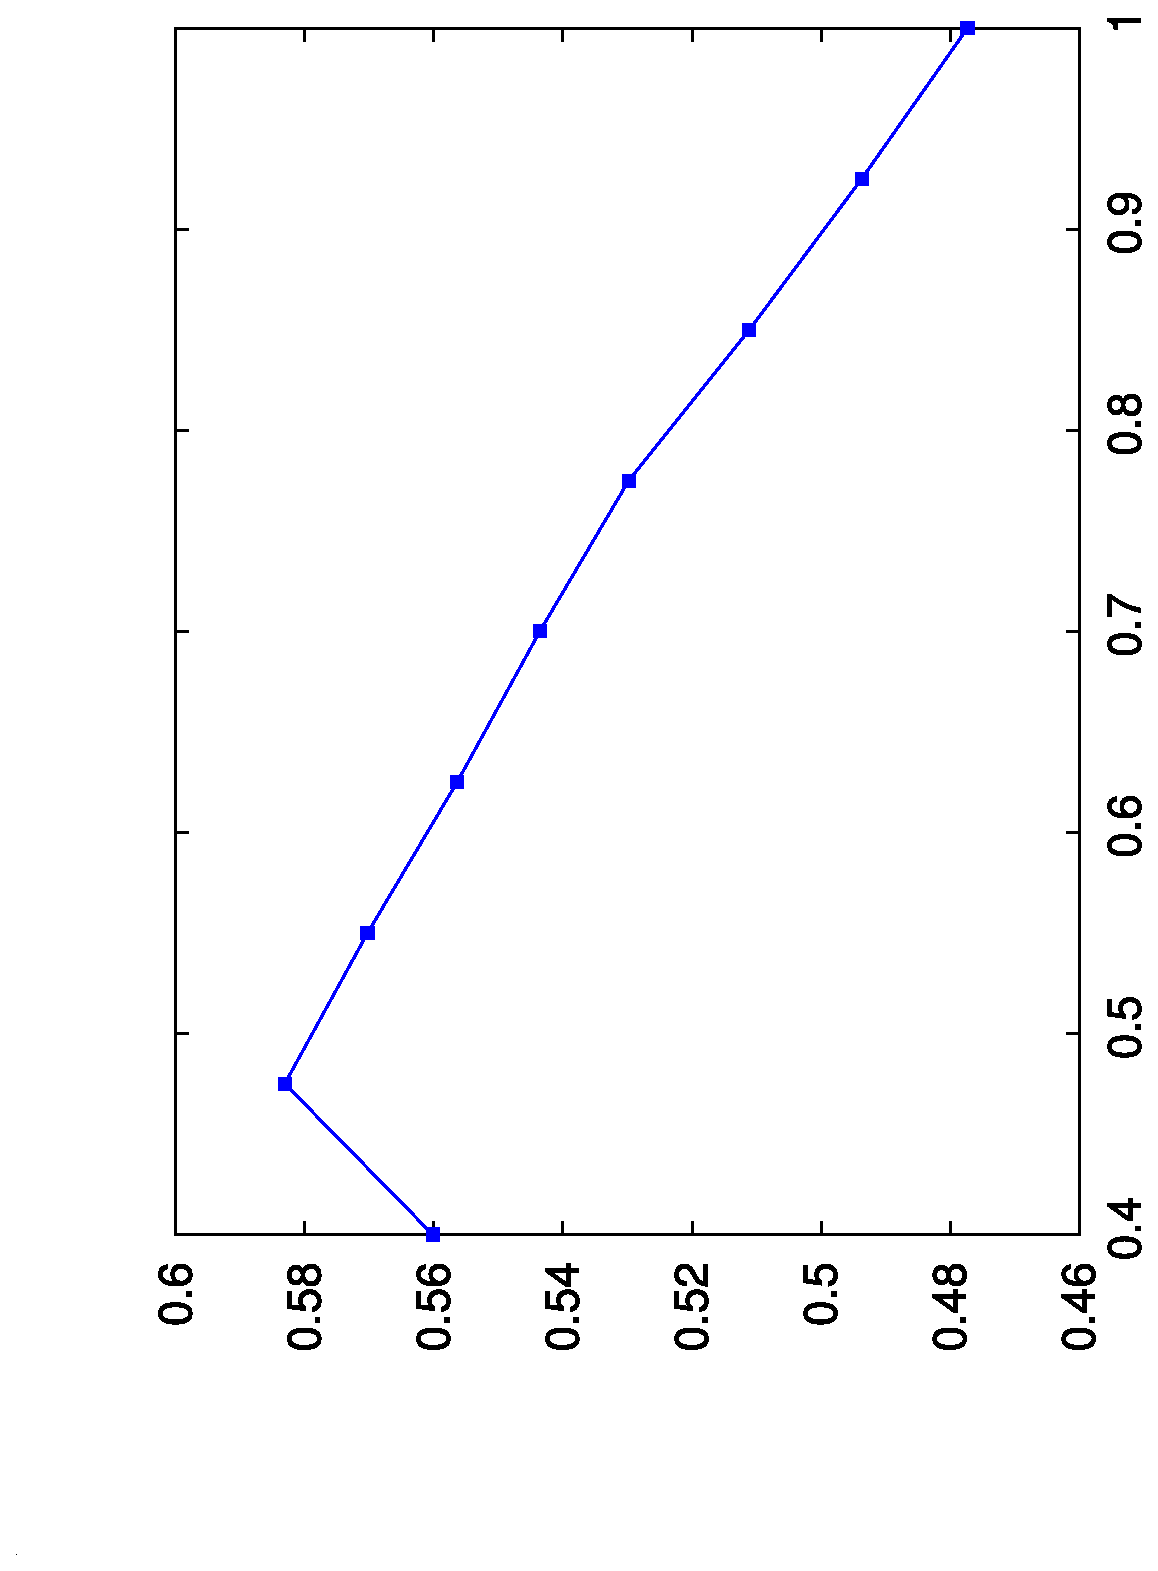
\includegraphics[width=0.73\textwidth,angle=-90]{figures/alphaomega-1.eps}
  \end{minipage} 
  \hfill
  \begin{minipage}[t]{0.49\textwidth}
  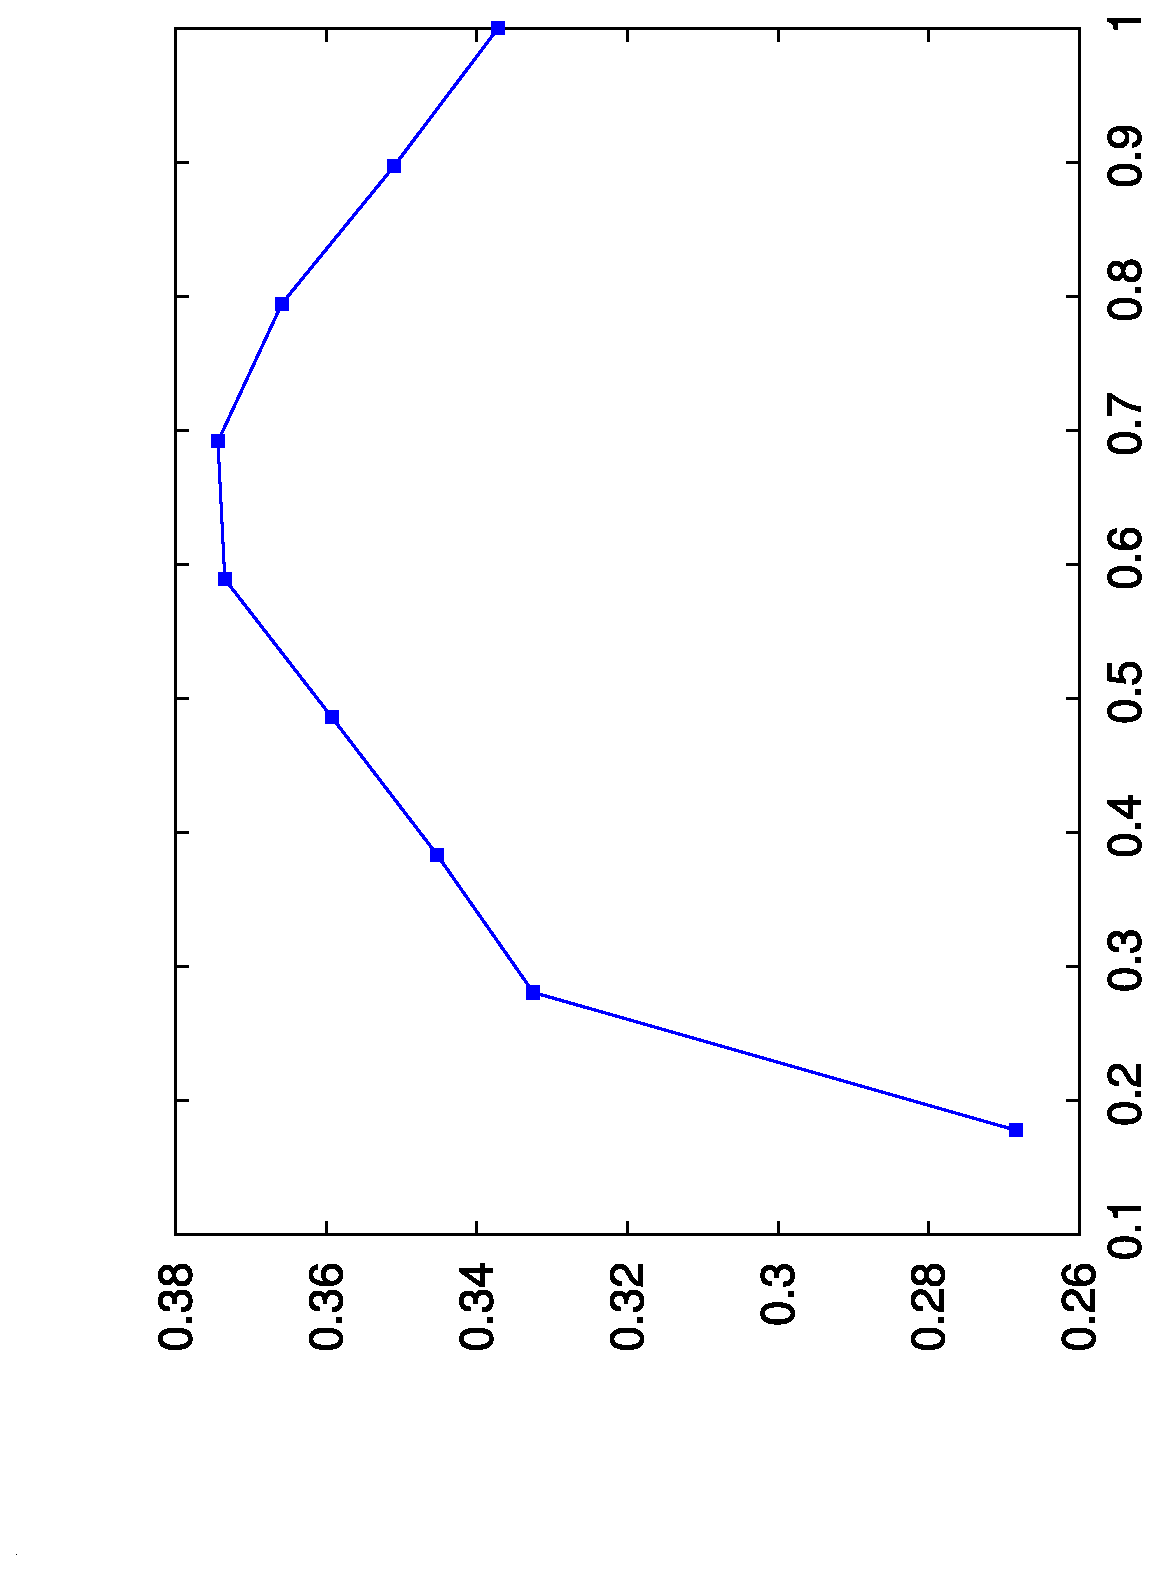
\includegraphics[width=0.73\textwidth,angle=-90]{figures/alphaomega-2.eps}
  \end{minipage}
  \caption{Relationship between $\omega$ and $\alpha^\omega_P\alpha^\omega_D$
           in two iterations of problem {\tt capri}.}
  \label{fig:alphaomega}
\end{figure}

In our crude linesearch procedure we choose 9 points uniformly 
distributed in the interval $[\alpha_P\alpha_D, 1]$ 
and evaluate, for each of these points, the stepsizes 
$\alpha^\omega_P$ and $\alpha^\omega_D$ in both spaces. 
When a larger stepsize $\alpha^\omega_P$ or $\alpha^\omega_D$ is obtained, 
the corresponding $\omega$ is stored as $\omega_P$ or $\omega_D$ 
respectively. Hence, we allow two different weightings for directions 
in the primal and dual spaces.

%
% Section
%
\section{Numerical results}
\label{NumRes}

We have implemented our proposal within the \HOPDM\ interior point solver 
\cite{HOPDM}. 
%
%Unlike Mehrotra and Li's approach, which generates Krylov directions and
%chooses weights and combines them into a composite direction, we
%generate a sequence of multiple centrality correctors.
%
We tested our implementation in a series of computational 
experiments, using test problems from different collections. 
As a comparison, we present the results obtained by \PCx\ \cite{PCx}, 
a reference implementation of interior point methods. Since the two 
implementations, \PCx\ and \HOPDM, have different termination criteria 
in their default configurations, for the purpose of consistency,
in the results shown, 
we decided to implement in \HOPDM\ the criteria used in the study 
performed by Mehrotra and Li \cite{MehrotraLi}.
Therefore, for all solvers optimal termination occurs when the conditions
(\ref{eq:TerminationCriteriaPCx}) are met, with feasibility
accuracy $p=8$ and complementarity accuracy $q = 10$.

We use $\gamma = 0.1$ in the definition of symmetric 
neighbourhood and define aspiration levels for the stepsizes using the rule
\[
  \tilde{\alpha}_{P} = \min(1.5 \alpha_{P} \! + \! 0.3, \, 1) 
  \quad \mbox{ and } \quad
  \tilde{\alpha}_{D} = \min(1.5 \alpha_{D} \! + \! 0.3, \, 1). 
\]
The values suggested in \cite{Gondzio96} were more conservative:
$\tilde{\alpha} = \min (\alpha + 0.1, \, 1)$.
Thanks to the weighting mechanism we can control 
the contribution of the corrector in an adaptive way,
and thus be more demanding in the definition of the aspired stepsizes.

Centrality correctors are accepted in the primal and/or dual space
if ${\alpha}_{P}^{new} \geq 1.01 \alpha_{P}$ 
and/or ${\alpha}_{D}^{new} \geq 1.01 \alpha_{D}$, respectively.

\fb{
Note that this is different from what described in \cite{Gondzio96}: there, 
a corrector is accepted if ${\alpha}^{new} \geq \alpha + \gamma\delta_\alpha$, 
where $\gamma = \delta_\alpha = 0.1$. What did HOPDM use to do?
}

We present our results in terms of number of iterations and number 
of backsolve operations. The rationale behind this decision is that 
the multiple centrality correctors technique determines the number 
of allowed correctors on the basis of the ratio between factorisation 
cost and backsolve cost. This ratio can be very different across 
implementations, and is mainly influenced by the linear algebra 
routines used. 
\HOPDM\ comes with an in-house linear algebra implementation, while
\PCx\ relies on the more sophisticated sparse Cholesky solver
of Ng and Peyton. Therefore, the \PCx\ code tends to use less 
correctors per iteration.
In all other respects, the correction scheme follows closely the one
of \HOPDM\ and the paper \cite{Gondzio96}.

%
%
\subsection{Mehrotra-Li test collection}
\label{ML-tests}

First we considered the test set used in \cite{MehrotraLi}: 
it contains 101 problems from both Netlib and Kennington collections. 
%
In Table~\ref{MLtotals} we present the computational comparison 
outlining the total number of iterations and the total number 
of backsolves necessary to solve the problems in Mehrotra and Li's test set. 
Column \HO\ displays the results obtained
by the previous implementation, while column d\HO\ reports
the results obtained by the current implementation of weighted
correctors with a default choice of the number of centrality correctors. 
The last column presents the relative change between the two 
versions of \HOPDM\ tested. 
As a reference, we also report in this table the overall
statistics of \PCx\ (release 1.1) on these problems. Also for \PCx\ we adopted
the termination criteria (\ref{eq:TerminationCriteriaPCx}),
with $p = 8$ and $q = 10$.
We found the number of backsolves by counting the number of calls 
to the functions {\tt IRSOLV()} and {\tt EnhanceSolve()}, for \HOPDM\ and
\PCx\ respectively.
%
\begin{table}[ht]
  \centering
  \begin{tabular}{|l|c||c|c|r|}\cline{2-5}
    \multicolumn{1}{c|}{}&\PCx & \HO& d\HO&\multicolumn{1}{c|}{Change}\\ \hline
    Iterations       & 2114 & 1871  & 1445           &   -22.77\% \\ 
    Backsolves       & 4849 & 6043  & 5717           &   -5.39\%  \\
    Backsolves/iter. & 2.29 & 3.23  & 3.95           &   +22.29\% \\ \hline
  \end{tabular}
  \caption{Overall results obtained on Mehrotra and Li's test collection.}
  \label{MLtotals}
\end{table}
%
\\From Table~\ref{MLtotals} we first observe the very small number 
of backsolves per iteration needed by \PCx. This is due to the fact 
that \PCx\ allows the use of Gondzio's multiple centrality correctors 
only in 4 problems: {\tt dfl001}, {\tt maros-r7}, {\tt pds-10} and 
{\tt pds-20}.
%
Also we notice that when we allow an adaptive weighting 
of the correctors there is a tendency to use more correctors 
per iteration than previously. 
This happens because the weighting mechanism makes it more likely
to accept some correctors that otherwise would have been rejected
as too aggressive.
While this usually leads to a decrease 
in iteration count, it also makes each iteration more expensive.

In Table~\ref{TimeML} we detail the problems for which we obtained savings 
in computational time. Given the small dimension of most of the problems 
in the Netlib collection, we did not expect major savings. However, as the
problem sizes increase, we can see that the proposed way of evaluating and
weighting the correctors pays off. This led us to investigate further 
the performance of the proposed implementation, which we will discuss
in Section~\ref{BN-tests}.
%
\begin{table}[ht]
  \centering
  \begin{minipage}[t]{0.36\textwidth}
    \begin{tabular}{|l|r|r|}\hline
      Problem & \multicolumn{1}{c|}{\HO} & d\HO \\ \hline
      bnl1    &   0.36 &   0.25 \\
      d{f}l001& 150.63 & 114.80 \\
      maros-r7&   7.76 &   7.52 \\
      pilot   &   5.23 &   4.35 \\ \hline
    \end{tabular}
  \end{minipage}
  \begin{minipage}[t]{0.36\textwidth}
    \begin{tabular}{|l|r|r|}\hline
      Problem & \multicolumn{1}{c|}{\HO} & d\HO\\ \hline
      pilot87 &  12.62 &  11.88 \\ 
      pds-06  &  24.59 &  21.31 \\
      pds-10  &  96.57 &  79.29 \\
      pds-20  & 923.71 & 633.64 \\ \hline
    \end{tabular}
  \end{minipage}
  \caption{Problems that showed time savings (times are in seconds).}
  \label{TimeML}
\end{table}

We were particularly interested in comparing the results produced by our 
weighted correctors approach with those published in \cite{MehrotraLi}. 
%
%A full comparison is presented in Table~\ref{MLresults}.
%In terms of the number of iterations, Mehrotra and Li's scheme is extremely 
%promising. 
% However, only 13 problems out of 101 showed a reduction 
% in computing time when using 4 Krylov directions. 
%
In the tables of results presented in \cite{MehrotraLi}, the best 
performance in terms of iteration count is obtained by \PCx 4, which 
uses 4 Krylov subspace vectors. These directions are combined with 
an affine-scaling predictor direction and Mehrotra's second-order 
correction, leading to 6 backsolves per iteration. 
%  {\bf (but it's not clear that they use Krylov 
%        directions and solve a linear subproblem at every iteration)}
This number increases when the linear subproblem produces an optimal 
objective value smaller than a specified threshold or the new iterate 
fails to satisfy some neighbourhood condition: in these cases 
the pure centering direction $\Delta_{cen} w$ also needs to be computed,
and a seventh backsolve is performed.

As we understand the paper \cite{MehrotraLi}, \PCx 0 uses exactly 
2 backsolves per iteration: one to compute the affine-scaling direction,
another to compute Mehrotra's corrector; \PCx 2 and \PCx 4 compute 
two and four additional Krylov vectors, hence they use
4 and 6 backsolves per iteration, respectively.
In columns \HO-0, \HO-2 and \HO-4, we present 
the results obtained by \HOPDM\ when forcing the use of 0, 2 and 4 
multiple centrality correctors. 
In the column called \HO\raisebox{.7pt}{-$\infty$} we report the results 
obtained when an unlimited number of correctors is allowed
(in practice we allow no more than 20 correctors).
The last column, labelled d\HO, presents the results obtained 
by the default way of choosing the number of correctors allowed.

Consequently, up to 2, 4 and 6 backsolves per iteration are allowed
in \PCx 0, \PCx 2 and \PCx 4 and in \HO-0, \HO-2 and \HO-4 runs, respectively.
The number of backsolves reported for \HOPDM\ includes two needed by 
the initialisation procedure: the number of backsolves 
should not exceed $2 \times {\rm {Its}} + 2$, 
$4 \times {\rm {Its}} + 2$ and $6 \times {\rm {Its}} + 2$ respectively
for \HO-0, \HO-2 and \HO-4.
The observed number of backsolves is often much smaller
than these bounds because the correcting mechanism switches off 
when the stepsizes are equal to 1 or when the corrector does not 
improve the stepsize. Problem {\tt afiro} solved by \HO-4 needs 24 
backsolves, 22 of which compute different components of directions, 
hence the average number of backsolves per iteration is only 22/6 
and is much smaller than 6. Occasionally,
as a consequence of numerical errors, certain components 
of direction are rejected on the grounds of insufficient accuracy:
in such case the number of backsolves may exceed the stated upper bounds.
The reader may observe for example that {\tt pilot4} is solved by \HO-4
in 16 iterations, but the number of backsolves is equal to 100 and 
exceeds $6 \times 16 + 2 = 98$.

The version \HO\raisebox{.7pt}{-$\infty$} requires 1139 iterations to solve 
the collection of 101 problems, an average of just above 11 iterations
per problem. This version has only an academic interest, 
yet it reveals a spectacular efficiency of interior point 
methods which can solve difficult linear programs of medium sizes 
(reaching a couple of hundred thousand variables) in just 
a few iterations.
In particular, it suggests that if we had a cheap way of generating
search directions, then it would be beneficial to have as many as possible.

%
%
\subsection{Beyond Netlib}
\label{BN-tests}

We have applied our algorithm to examples from other test collections 
besides Netlib.
These include other medium to large linear programming problems, 
stochastic problems and quadratic programming problems.

We used a collection of medium to large problems taken from different
sources: problems {\tt CH} through {\tt CO9}
are MARKAL (market allocation) models; {\tt mod2} through {\tt worldl} are
agricultural models used earlier in \cite{Gondzio96}; problems {\tt route}
through {\tt rlfdual} can be retrieved from 
\begin{center}
{\tt http://www.sztaki.hu/\~{}meszaros/public\_ftp/lptestset/misc/},
\end{center}
problems {\tt neos1} through {\tt fome13} can be retrieved from 
\begin{center}
{\tt ftp://plato.asu.edu/pub/lptestset/}.
\end{center}

In Table~\ref{TimeBN} we detail the sizes of these problems and provide 
a time comparison between our previous implementation (shown in column
\HO), and the current one (in column d\HO).
This test collection contains problems large enough 
to show a consistent improvement in CPU time: in only 4 problems 
({\tt mod2}, {\tt dbc1}, {\tt watson-1}, {\tt sgpf5y6}) 
we recorded a deterioration of the performance by more than 1 second.
The improvements are significant on problems with a large 
number of nonzero elements. In these cases, d\HO\
produces savings from about 10\% to 30\%, with the remarkable results
in {\tt rail2586} and {\tt rail4284}, for which the relative savings 
reach 45\% and 65\%, respectively.

More numerical results obtained on some collections of stochastic
programming problems and quadratic problems can be found in
\cite{ColomboGondzio05}.

\begin{small}
\begin{longtable}{|l|rrr|r|r|r|} \hline 
  \multicolumn{1}{|c|}{Problem}
& \multicolumn{1}{c}{Rows}
& \multicolumn{1}{c}{Cols}
& \multicolumn{1}{c|}{Nonzeros}
& \multicolumn{1}{c|}{\HO}
& \multicolumn{1}{c|}{d\HO}
& \multicolumn{1}{c|}{Change}\\ \hline
\endhead
\hline
\multicolumn{7}{c}{\raisebox{-1ex}{Table~\ref{TimeBN}: Time comparison on 
other large problems (times are in seconds).}}
\endfoot
\label{TimeBN}
CH & 3852 & 5062 & 42910 & 1.03 & 1.23 & 19.4\% \\
GE & 10339 & 11098 & 53763 & 5.72 & 5.46 & -4.5\% \\
NL & 7195 & 9718 & 102570 & 4.37 & 3.95 & -9.6\% \\
BL & 6325 & 8018 & 58607 & 2.15 & 2.14 & -0.5\% \\
BL2 & 6325 & 8018 & 58607 & 2.35 & 2.31 &  -1.7\% \\
UK & 10131 & 14212 & 128341 & 2.48 & 3.21 &  29.4\% \\
CQ5 & 5149 & 7530 & 83564 & 2.54 & 2.60 &  2.4\% \\
CQ9 & 9451 & 13778 & 157598 & 9.67 & 8.84 &  -8.6\% \\
CO5 & 5878 & 7993 & 92788 & 3.16 & 3.59 &  13.6\% \\
CO9 & 10965 & 14851 & 176346 & 21.10 & 15.35 & -27.3\% \\
mod2 & 35664 & 31728 & 220116 & 20.59 & 21.68 & 5.3\% \\
world & 35510 & 32734 & 220748 & 26.35  & 23.41 & -11.2\% \\
world3 & 36266 & 33675 & 224959 & 31.13 & 27.49 & -11.7\% \\
world4 & 52996 & 37557 & 324502 & 73.21 & 56.14 & -23.3\% \\
world6 & 47038 & 32670 & 279024 & 39.33 & 32.79 & -16.6\% \\
world7 & 54807 & 37582 & 333509 & 43.14 & 36.02 & -16.5\% \\
worldl & 49108 & 33345 & 291942 & 43.95 & 36.82 & -16.2\% \\
route & 20894 & 23923 & 210025 & 40.92 & 33.78 & -17.4\% \\
ulevi & 6590 & 44605 & 162207 & 9.04 & 9.55 & 5.6\% \\
ulevimin & 6590 & 44605 & 162207 & 16.52 & 16.46 & -0.4\% \\
%aircraft & 3754 & 7517 & 24034 & 0.28 & 0.32 &  14.3\% \\
dbir1 & 18804 & 27355 & 1067815 & 162.18 & 146.51 & -9.7\% \\
dbir2 & 18906 & 27355 & 1148847 & 208.93 & 156.11 & -25.3\% \\
dbic1 & 43200 & 183235 & 1217046 & 72.96 & 77.31 & 5.9\% \\
pcb1000 & 1565 & 2428 & 22499 & 0.26 & 0.33 & 26.9\% \\
pcb3000 & 3960 & 6810 & 63367 & 1.13 & 1.16 & 2.7\% \\
rlfprim & 58866 & 8052 & 265975 & 15.63 & 15.08 & -3.5\% \\
rlfdual & 8052 & 66918 & 328891 & 71.17 & 49.79 & -30.0\% \\
neos1 & 131581 & 1892 & 468094 & 169.11 & 141.89 & -16.1\% \\
neos2 & 132568 & 1560 & 552596 & 113.86 & 86.13 & -24.4\% \\
neos3 & 132568 & 1560 & 552596 & 132.02 & 120.59 & -8.7\% \\
neos & 479119 & 36786 & 1084461 & 1785.80 & 1386.58 & -22.4\% \\
watson-1 & 201155 & 383927 & 1053564 & 138.60 & 166.21 & 19.9\% \\
sgpf5y6 & 246077 & 308634 & 902275 & 49.58 & 64.45 & 30.0\% \\
stormG2-1000 & 528185 & 1259121 & 4228817 & 1661.54 & 1623.19 & -2.3\% \\
rail507 & 507 & 63009 & 472358 & 9.77 & 10.10 & 3.4\% \\
rail516 & 516 & 47311 & 362207 & 7.59 & 5.89 & -22.4\% \\
rail582 & 582 & 55515 & 457223 & 9.67 & 9.60 & -0.7\% \\
rail2586 & 2586 & 920683 & 8929459 & 1029.36 & 566.82 & -44.9\% \\
rail4284 & 4284 & 1092610 & 12372358 & 2779.63 & 978.48 & -64.8\% \\
fome11 & 12142 & 24460 & 83746 & 407.20 & 265.21 & -34.9\% \\
fome12 & 24284 & 48920 & 167492 & 766.96 & 508.61 & -33.7\% \\
fome13 & 48568 & 97840 & 334984 & 1545.05 & 990.62 & -35.9\% \\
%\hline Totals  & & & & 11537.03  & 7713.8 \\
\end{longtable} 
\end{small}

In Figure~\ref{fig:PerfProfile}, we show the CPU-time based 
performance profile \cite{DolanMore} for the two algorithms. 
This graph shows the proportion of problems that each algorithm
has solved within $\tau$ times of the best. Hence, for
$\tau = 1$ it indicates that d\HO\ has been the best solver on 72\%
of the problems, against 28\% for \HO. For larger values of $\tau$,
the performance profile for d\HO\ stays above the one for \HO, thus
confirming its superiority. In particular, it solves all problems
within 1.3 times of the best.
%
\begin{figure}[ht]
  \centering
  \includegraphics[width=0.75\textwidth]{figures/perfprof-BN.eps}
  \caption{Performance profile for \HO\ and d\HO\ on the set of problems
    of Table~\ref{TimeBN}.}
  \label{fig:PerfProfile}
\end{figure}

% The collection of stochastic programming problems contains 119 examples
% and comes from
% \begin{center}
% {\tt http://www.sztaki.hu/\~{}meszaros/public\_ftp/lptestset/stochlp/}. 
% \end{center}
% 
% We have also tested the implementation on a collection of 29 quadratic 
% programming problems, available from
% \begin{center}
% {\tt http://www.sztaki.hu/\~{}meszaros/public\_ftp/qpdata/}.
% \end{center}
%
% Normally, HOPDM automatically chooses between direct and iterative 
% approaches for computing directions. A higher-order correcting scheme
% makes much more sense with the direct approach when 
% backsolve is significantly less expensive than the factorisation.
% In order to maintain consistency, we forced HOPDM to use a direct 
% approach when 
% solving this class of problems, rather than an iterative scheme.

%
% Section
%
\subsection{Conclusions}
\label{Conclusions}

In this paper we have revisited the technique of multiple centrality 
correctors \cite{Gondzio96} and added a new degree of freedom to it. 
Instead of computing the corrected direction from 
$\Delta w = \Delta_p w + \Delta_c w$ where $\Delta_p w$ and $\Delta_c w$ are 
the predictor and corrector terms, we allow a choice of weight 
$\omega \in (0,1]$ for the corrector term and compute 
$\Delta w = \Delta_p w + \omega \Delta_c w$.
We combined this modification with the use of a symmetric neighbourhood
of the central path. We have shown that the use of this neighbourhood
does not cause any loss in the worst-case complexity of the algorithm. 

The computational results presented for different classes of problems 
demonstrate the potential of the new scheme. We have compared our algorithm 
against the recently introduced Krylov subspace scheme \cite{MehrotraLi}.
The two approaches have similarities: they look for a set of attractive 
independent terms from which the final direction is constructed. 
Mehrotra and Li's approach uses the first few elements from the basis
of the Krylov space; our approach generates direction terms using 
centrality correctors of \cite{Gondzio96}. Mehrotra and Li's approach 
solves an auxiliary linear program to find an optimal combination 
of all available direction terms; our approach repeatedly chooses 
the best weight for each newly constructed corrector term (and switches 
off if the use of the corrector does not offer sufficient improvement). 
Eventually, after adding $k$ corrector terms, 
the directions used in our approach have form
\[
  \Delta w = \Delta_a w + \omega_1\Delta_1 w + \ldots + \omega_k\Delta_k w,
\]
and the affine-scaling term $\Delta_a$ contributes to it without any
reduction. Hence, the larger the stepsize, the more progress we make
towards the optimizer.

The comparison presented in Section~\ref{ML-tests} shows a clear advantage 
of our scheme over that of \cite{MehrotraLi}. Indeed, with the same 
number of direction terms allowed, our scheme outperforms Krylov subspace 
correctors by a wide margin. Multiple centrality correctors show 
consistent excellent performance on other classes of problems
including medium to large scale linear programs beyond the Netlib 
collection and medium scale quadratic programs.

\fb{
Monteiro, Adler and Resende \cite{MonteiroAdlerResende90} talk about
corrector steps.
}

\fb{
It would be good to try and implement using the search direction from
the previous iteration as another (free) direction to span the subspace.
}

\begin{remark}
From the study of subspace searches it is clear that the more 
directions we consider, the better the final search direction 
we get. Therefore, if we had a cheap way of generating search
directions (rather than from solving a system of linear equations),
then these should be employed.
\end{remark}

\begin{remark}
Mehrotra and Li \cite{MehrotraLi} mention employing previous search
directions alongside the usual ones. The use of these incurs an
increased memory usage, but no additional computational cost.
However, it does not seem that they were actually employed in
the runs. This opens some questions on what constitutes a valid
previous direction (only affine scaling, the final composite direction
or something else).
\end{remark}


\chapter[Warm-start strategies for stochastic linear programs.]{Warm-start strategies for \\stochastic linear programs.}
%Started on Monday 28 August 2006
%Aug: 29, 30
%Sep:  7,  8, 13
% 2007
%Feb:  4
%Mar:  8, 18, 19, 20, 28, 30
%Apr:  2,  3,  4,  5, 18, 21, 28, 30
%May:  1,  4,  6,  8

%
% Chapter: Warm-start
%
\label{ch:Warmstart}

In this chapter we develop an efficient way of constructing a 
starting point for large-scale stochastic linear programs.
We first present the relevant
concepts of stochastic programming, stressing the fact that
they lead to highly structured problems.
Then we introduce 
the proposed method of generating an advanced starting point for 
stochastic programming that exploits the inherent structure of the
problem. Finally, we present an analysis of the warm-start strategy.
The results presented in this chapter have been the subject
of a joint work with Jacek Gondzio and Andreas Grothey
\cite{ColomboGondzioGrothey06}. 


%
% Section
%
\section{Stochastic programming}

Stochastic programming \cite{BirgeLouveaux,KallWallace}
is a technique to help decision-making 
in many areas of applied mathematics, logistics, engineering, economics and 
finance where some parameters are unknown.

\ignore{
In a large scenario tree there may be very little difference among 
scenarios, and so the large-scale problem can provide a fine-grained 
solution to a problem that could have been solved more coarsely by 
using a much smaller tree. This observation suggests a
warm-start technique that can be applied in the context of interior 
point methods. A warm-start solution is obtained by solving the 
stochastic optimization problem for a reduced event tree, the dimension
of which is much smaller than that of the complete one. The solution 
to the reduced problem is used to construct an advanced iterate for 
the complete formulation. We provide evidence that this novel way 
of exploiting the problem structure to generate an initial iterate
provides a better starting point (in terms of centrality, feasibility, 
and closeness to optimality) than the one produced by a generic 
strategy.
}

By stochastic programming, we mean decision and control models in which 
data evolves over time, and are subject to significant uncertainty.
%
Uncertainty in the data is a commonly observed phenomenon in
optimization problems coming from applications. Uncertainty
affects problems that aim to plan future actions based on forecasted
prices or costs. In can be argued that nearly all practical
optimization problems display uncertainty in the data, even if this is
not made explicit in the chosen solution method. 

\ignore{
A crude approach to the problem of optimization under uncertainty
has been to replace the uncertain data by their expected value and
solve an {\em average case} problem. However, this approach is not
suitable when some sort of provision of hedging against risk has to be
taken into account. Another popular approach is {\em Robust
optimization}, or the optimization of the {\em worst case}
scenario \cite{KallWallace}. 
}

When the uncertainty cannot be conveniently forecasted, the use of 
deterministic models is considered inadequate for decision making. In 
these situations, being able to describe and model the uncertain parameters
becomes a requirement for robust decision making. Stochastic 
programming is the discipline that 
studies the methods and provides the tools for modelling uncertainty.

Stochastic programming models uncertainty through the analysis 
of possible future outcomes (scenarios). 
As the robustness of the decisions taken increases with the detail of the 
description, this encourages the generation of very large scenario trees.
Stochastic programming aims to take all possible future scenarios 
into account, weighting them
with their respective probabilities. Its strength lies in the
adaptability which allows to express preferences such as restricting
the exposure to risk. Unlike alternative approaches, it allows to model
situations in which possible future events are correlated or follow a
time-structure, in that realisations become known in stages and it is
possible to react to the observed events.

The stochastic programming paradigm is perceived to have
some weaknesses.
In particular, these relate to the need for reliable forecasts
of the probabilities of the future events under consideration
(which may not be available), and the fact that 
taking into account a large number of possible scenarios 
(especially when applied to multi-stage models) leads to
to the generation of large-scale structured optimization problems,
the solution of which is challenging. 
With the growing industrial acknowledgement of the benefits of 
considering uncertainty for planning purposes, it is expected that the 
need for solving very large instances will grow as well.

As the dimensions of the problems increase, the computational advantages 
of relying on interior point solvers become more and more evident. 
Very-large-scale problems, however, create more than one difficulty to general 
purpose solvers.
Problems of such sizes can be solved provided they are not only sparse,
but also structured. If that is the case, then the structure present 
in the matrix should be conveniently exploited.
The easier access to powerful parallel machines leads to a 
further advantage coming from assigning the computational work 
to more than one processing unit through the parallelisation of 
the linear algebra.
This is where structure-exploiting parallel solvers such as \OOPS 
\cite{GondzioSarkissian} excel. Moreover, structure-exploiting interior 
point methods can be used not only for linear programming problems, 
but also for quadratic and nonlinear problems \cite{GondzioGrothey07}.

%
%
\subsection{Stochastic programming concepts}

A stochastic programming problem incorporates the uncertain parameters
in the model. 
Following \cite{BirgeLouveaux}, this can be illustrated by the 
{\em two-stage stochastic problem}
%
\be  \label{eq:SP1}
  \begin{array}{rl}
    \min        & (q^1)^T x^1 + \E_\xi Q(x^1, \xi) \\
    \mbox{s.t.} & W^1x^1 = h^1,  \\
                & x^1\geq 0, \\
  \end{array}
\ee
%
where $\xi$ is a random variable, $\E_\xi$ is the expectation function
and
\be  \label{eq:SP2}
  \begin{array}{rcrl}
  Q(x^1,\xi)& \!\!\! = \!\!\! & \min & q(\xi)^T y(\xi) \\
            &   & \mbox{s.t.} & W(\xi)y(\xi) = h(\xi) - T(\xi)x^1, \\
	    &   &             & y(\xi) \ge 0.
  \end{array}
\ee
Notice that we use the convention that first-stage variables
and coefficients carry the superscript 1.
Problem \eqref{eq:SP1}-\eqref{eq:SP2} can be interpreted as an optimization
problem in which some parameters or coefficients are unknown.
While (\ref{eq:SP1}) models the first stage decisions, 
(\ref{eq:SP2}) refers to the second stage decisions, which can
be made only after a realisation of the random variable $\xi$
has become known. Note how the first-stage decision variables $x^1$ 
appear in (\ref{eq:SP2}): at the time when the realisation
become available, the first-stage decisions have already been made.

In stochastic programming, the uncertain environment is 
described through a stochastic process which is assumed to be 
known or can be either estimated from historical data or 
conjectured according to some prescribed properties. The 
continuous process $\xi$ is usually further approximated by a discrete 
distribution
in order to obtain a computationally amenable description. 
In such a case, the most common techniques
\cite{HoylandKautWallace,Pflug01} generate a 
finite, but usually very large, number of scenarios that represent an 
approximate description of the possible outcomes.

The model can be generalised to a {\em multi-stage model} in which 
the evolution of uncertainties can be 
described as an alternating sequence of decisions and random 
realisations that occur at different stages.
A multi-stage stochastic program with recourse is a multi-period 
mathematical program where parameters are assumed to be uncertain 
along the time path.
The stages do not necessarily refer to time periods, but they correspond
to steps in the decision process. In particular, at each stage the
realisations of some random parameters become known, and a decision
must be taken.
The main interest lies in the 
first-stage decisions which consist of all decisions that have to
be made before the information is revealed. Later-stage decisions 
are allowed to adapt to the information that has become available 
up to that point.

The discrete stochastic process can be represented as an 
{\em event tree} $\Ctree$,
where each node denotes a stage when a realisation 
of the random process becomes known and a subsequent decision is taken.
It is common to consider balanced trees, where the number of
branches for each node is the same at each stage.
However, a better approach is to consider more branches in the
earlier stages than in the later ones. This leads to the
so-called {\em left-heavy trees}.
A very simple event tree is shown in Figure~\ref{fig:EventTree}.
%
\begin{figure}[ht]
  \begin{center}
    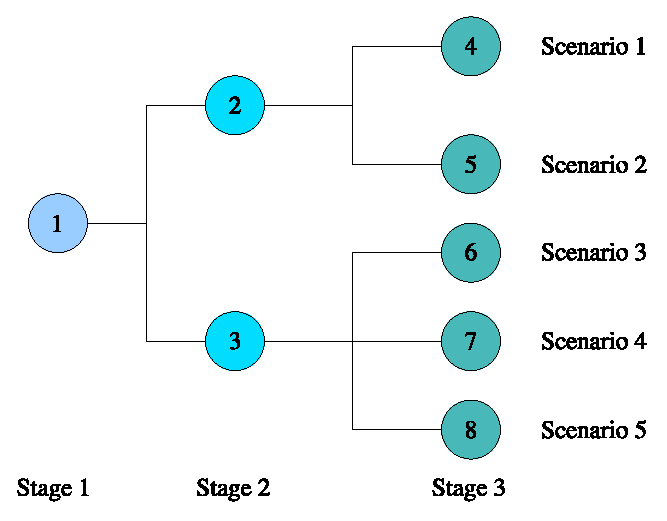
\includegraphics[scale=0.6]{figures/tree.eps}
    \caption{Event tree.}
    \label{fig:EventTree}
  \end{center}
  \vspace{-3ex}
\end{figure}

To each node of the event tree we associate a set of constraints, an 
objective function, and the conditional probability of visiting the 
node from its parent node in the previous stage.
A path from the root to a leaf node of the event tree represents a 
scenario.
The probability of each scenario is the product of the 
conditional probabilities of visiting each node on the path.

As we have already mentioned, usually a very large number of scenarios is
needed to adequately capture the characteristics of the underlying
continuous distribution, particularly in the multi-stage setting.
In this case, the number of scenarios grows exponentially with the
number of decisions considered at each stage.
The question of how to generate an appropriate scenario tree
is not trivial, and has received extensive attention in the
literature 
\cite{DupacovaConsigliWallace,HoylandKautWallace,HoylandWallace,Pflug01}.

%
%
\subsection{The deterministic equivalent formulation}
\label{DetEqForm}

A natural formulation of a stochastic programming problem relies on 
recursion to describe the dynamics of the modelled process.
The term {\it recourse} means that, at each stage, the decision 
variables adapt to the different outcomes of the random parameters.
For ease of presentation, we consider the linear version of the
recourse problem:
%
\be \label{eq:SLPRecourse}
\begin{array}{rl}
  \min & (q^1)^T x^1 + \E_\xi[\min\, q(\xi)^T y(\xi)] \\
  \text{s.t.} &  W^1x^1                   = h^1,      \\
	      &  T(\xi) x^1 + W(\xi) y(\xi) = h(\xi), \\
	      &  x^1 \geq 0,\; y(\xi) \ge 0,
\end{array}
\ee
%
where $y(\xi)$ denotes the recourse action which depends on the 
outcome of the random process $\xi$. 
Note that (\ref{eq:SLPRecourse}) combines in a single formulation
both (\ref{eq:SP1}) and (\ref{eq:SP2}).
After discretizing $\xi$ 
according to $P(y^i=\xi_i) = p^i$, and using the notation 
$T^i = T(\xi_i)$ (and analogously for $h^i$, $W^i$, $y^i$ and $q^i$), 
$i = 2, \ldots, n$,
problem (\ref{eq:SLPRecourse}) can be written in the 
{\em deterministic equivalent formulation}:
\be \label{eq:DetEq-2stage}
\begin{array}{rlllll}
\min & (q^1)^T x^1 + \displaystyle\sum_{i=2}^n p^i(q^i)^T y^i \\
\mbox{s.t.} & W^1x^1          &        &          & = h^1, \\
            & T^2x^1 + W^2y^1 &        &          & = h^2, \\
	    & \quad\vdots     & \hspace{-1em}\ddots & & \;\vdots \\
            & T^n x^1         &        &+\; W^ny^n & = h^n,\\
            & x^1 \geq 0,\; y^i \ge 0.
\end{array}
\ee
The deterministic equivalent formulation is derived by writing
explicitly each possible realisation of the random parameters.
The formulation (\ref{eq:DetEq-2stage}) does not have any stochasticity
left, but is completely deterministic, and is therefore a common
linear programming problem of (very) large dimensions.
Also note that problem (\ref{eq:DetEq-2stage}) displays a
dual-block angular structure
in the constraint matrix.

The same approach can be immediately extended to multi-stage models.
To formulate the deterministic equivalent of the multi-stage 
stochastic programming problem we first need to enumerate all nodes 
of the event tree. We use a breadth-first 
search order, i.e., we start from a root node corresponding 
to the initial stage and end with leaf nodes corresponding 
to the last stage. In this case, the constraint matrix displays
a nested dual-block angular structure.

Let $t = 1,2,\ldots,T$ denote the stage and let $\mathcal{L}_t$ 
be the set of nodes at stage $t$.
With $a(l)$ we denote the direct ancestor of node $l\in\mathcal{L}_t$ 
(which is a node that belongs to stage $t-1$), and with
$\mathcal{D}_l\subset\mathcal{L}_{t+1}$ the set of children of node $l$.
The decision variables are superscripted with the node number $l$;
similar notation is used for the corresponding matrix and vector blocks.
The total number of scenarios is $N$.

In the case of one-period recourse, 
the main constraint that describes the dynamics of the system has the form 
\[
  T^{l}x^{a(l)} +W^{l}x^{l} =h^{l}, \qquad l \in\mathcal{L}_t,\; t=2,\ldots,T,
\]
%
where $T^{l}$ is the technology matrix that varies 
with the node in the event tree, and $W^{l}$ is the recourse
matrix that, in general, depends on realisations within the same stage,
but often varies only with time.

The deterministic equivalent formulation of the multi-stage 
problem has the following general form:
\begin{equation}  \label{DetEquiv}
  \begin{array}{rlcll}
  \min & \displaystyle\sum_{t=1}^T\sum_{l\in\mathcal{L}_t} p^l (q^l)^T x^{l}\\
  \mbox{s.t.} & W^1 x^1            & \hspace{-1.5em} = h^1, \\
    & T^{l} x^{a(l)} + W^{l} x^{l} & \hspace{-1.5em} = h^{l}, 
                               &\quad l\in\mathcal{L}_t,\; t = 2,\dots,T, \\
    & \hspace{5.3em} x^{l}         & \hspace{-1.5em} \geq 0,
                               &\quad l\in\mathcal{L}_t,\; t = 1,\dots,T. \\
  \end{array}
\end{equation}

Note that the probabilities in the objective function of problem 
(\ref{DetEquiv}) are the unconditional path probabilities: $p^l$ is 
the probability that a path goes through node $l$, which equals the 
product of the conditional probabilities along the path from the root 
to node $l$.
Clearly, (\ref{DetEquiv}) represents a structured linear program. Its 
structure should be exploited in the solution algorithm.

If the event tree is traversed with depth-first-search ordering of the 
nodes during the generation of the mathematical program, the 
corresponding constraint matrix displays a nested dual block-angular 
structure.
Figure~\ref{fig:deteq} displays the two possible structures 
for the event tree of Figure~\ref{fig:EventTree} according 
to the chosen ordering of nodes.
%
\begin{figure}[ht]
  \centering
    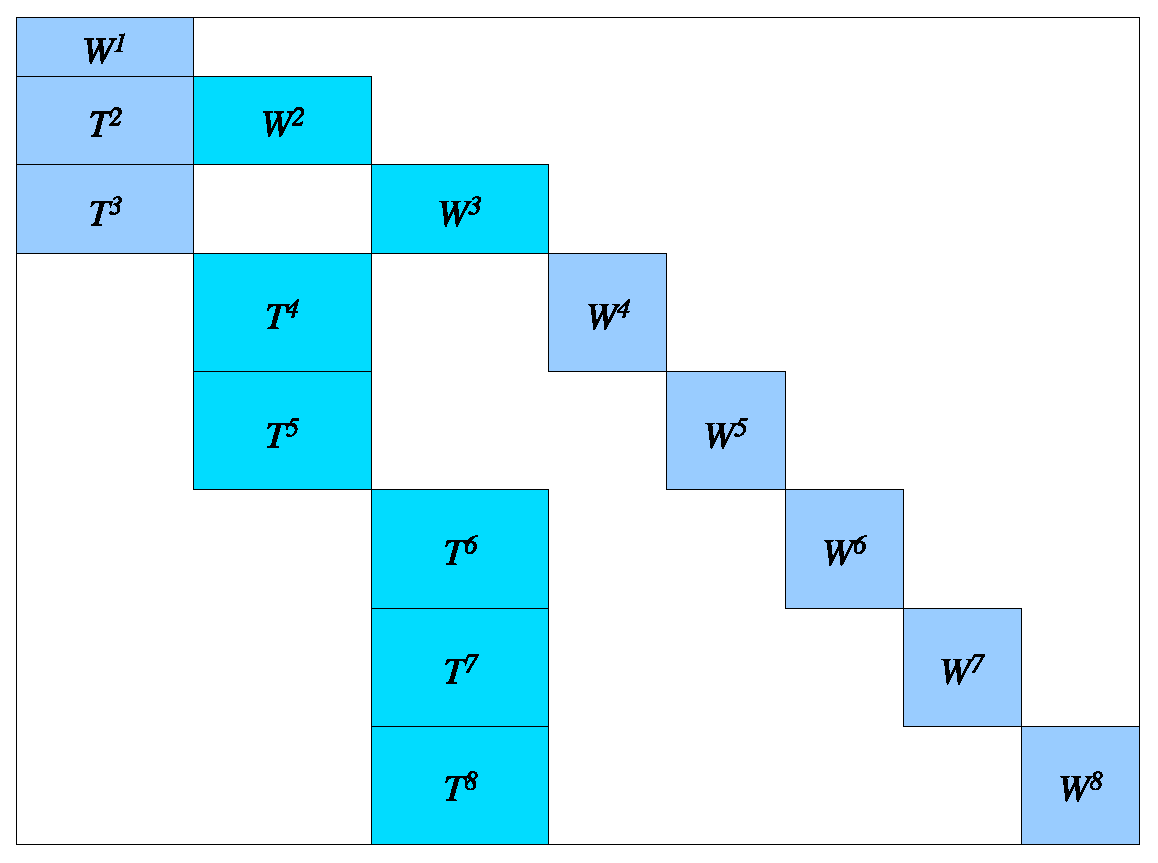
\includegraphics[scale=0.37]{figures/deteq-bfs.eps} \hfill
    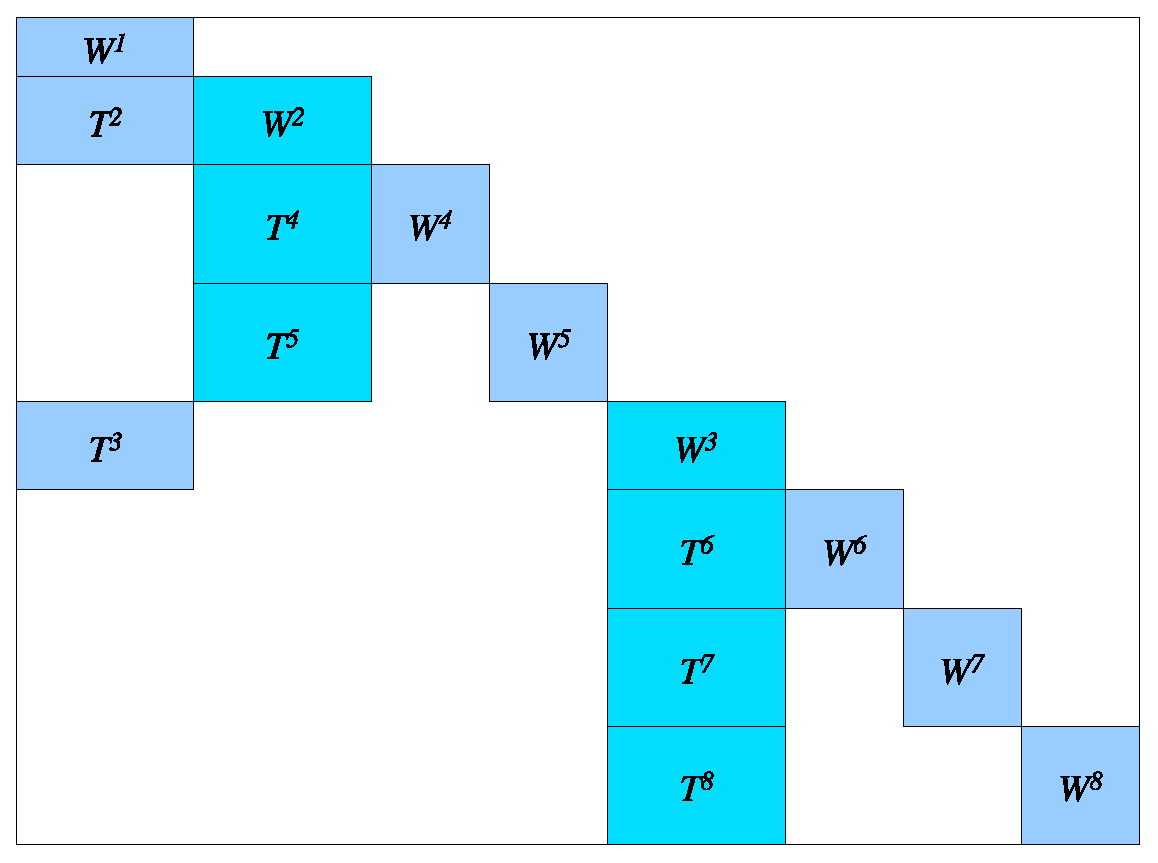
\includegraphics[scale=0.37]{figures/deteq-dfs.eps}
    \caption{Deterministic equivalent corresponding to the event tree 
             of Figure~\ref{fig:EventTree}, with nodes listed in breadth-first 
             order (left) and depth-first order (right).}
    \label{fig:deteq}
\end{figure}
%
While the different ordering of blocks whithin the matrix is not 
relevant for general-purpose solvers, the structure-exploiting
software \OOPS \cite{GondzioGrothey07,GondzioSarkissian} can take 
full advantage of the nested dual-block angular structure resulting
from the depth-first ordering in its internal object-oriented
linear algebra representation.

Several solution methods for stochastic linear programs have been 
presented in the literature. These often rely on some decomposition
approach \cite{Birge85,LinderothWright03,MulveyRuszczynski}, among others.
Kall and Mayer \cite{KallMayer} provided a comparison of different
solution algorithms for stochastic linear programming problems.
In what follows, instead, we consider solving the deterministic equivalent
problem directly through an interior point method.


%
% Section
%
\section{A reduced-tree warm-start iterate}
\label{sec:ReducedTree}

We already surveyed warm-start strategies in Section~\ref{sec:WarmStart}.
While those strategies apply to
general linear problems, we introduce an approach tailored to
stochastic programming. In particular, we propose to exploit the structure
inherent to a stochastic programming problem to generate a good 
warm-start iterate.

In the event tree corresponding to a large multistage program, 
the numerous leaf nodes descend from a relatively small number of 
branches in the first few stages. Two ``neighbouring'' scenarios, 
that is two scenarios that have common nodes, may display large 
differences concerning later stage decisions, but the decisions 
taken in the earlier stages are identical (nonanticipativity).
Moreover, there may be very little difference among 
scenarios, and so the large-scale problem can provide a fine-grained 
solution to a problem that could have been solved more coarsely by 
using a much smaller tree. 

These observations suggests a
warm-start technique that can be applied in the context of interior 
point methods. A warm-start solution is obtained by solving the 
stochastic optimization problem for a reduced event tree, whose 
dimension is much smaller than that of the complete one. The solution 
to the reduced problem is used to construct an advanced iterate for 
the complete formulation. We provide evidence that this novel way 
of exploiting the problem structure to generate an initial point 
provides a better iterate (in terms of centrality, feasibility, 
and closeness to optimality) than the one produced by a generic 
strategy.

Techniques for reducing the size of the scenario tree have been studied 
before from a probabilistic perspective; in some cases considerable 
savings can be obtained with such methods. Among others, 
Dupa\v{c}ov{\'a} \etal \cite{Dupacova} discuss an optimal scenario 
reduction technique that couples a large reduction of the scenario 
tree with a small loss in accuracy. In their example, a reduction by 
50\% of the scenario tree still maintains about 90\% of the original 
accuracy.
In this paper, we are interested in capturing some aspects of the 
stochasticity of the event tree without assuming further knowledge on 
the underlying stochastic process that generated it. Given this difference 
from what is required for example by \cite{Dupacova}, we will use less 
sophisticated arguments in finding a reduced tree.
We remark that if we have knowledge of the underlying stochastic process,
then we could exploit it in the generation of the reduced tree.

We first study how to build a reduced tree by choosing just 
some of the possible scenarios. We provide some insight on how to make 
this selection, so that our choice performs better than an arbitrary 
one.
Then we discuss how to obtain a warm-start solution from the reduced 
tree that corresponds to the chosen scenarios.
Our aim is to generate a warm-start iterate that allows to solve to 
optimality the complete problem in fewer iterations (and less computing 
time) than by a standard starting point heuristic \cite{Mehrotra92}.
With these aims, we propose a way of choosing a subset of scenarios 
that we believe to be sufficiently representative of the whole tree.
The algorithm can be summarised in the steps of
Algorithm~\ref{alg:OverallAlgorithm}.
%
\begin{algorithm}[h]
  \caption{Reduced-tree warm-start algorithm}
  \begin{algorithmic}[0]  \label{alg:OverallAlgorithm}
    \REQUIRE The complete event tree $\Ctree$.
    \smallskip
    \STATE Generate a reduced event tree $\Rtree\subset\Ctree$;
    \smallskip
    \STATE Solve the corresponding deterministic equivalent with a loose 
           tolerance;
    \smallskip
    \STATE Use this solution to construct a warm-start iterate for the 
    complete problem;
    \smallskip
    \STATE Solve the complete problem to optimality.
  \end{algorithmic}
\end{algorithm}

In the rest of this section we define our method of generating a 
reduced tree and describe the construction of the complete warm-start 
iterate.

%
%
\subsection{Scenario distance}
\label{sec:ScenarioDistance}

For the purposes of generating a reduced scenario tree (see
Section~\ref{sec:ReducedTreeGeneration}), we need to define a measure 
of distance between scenarios.
Recalling that a scenario is a path in the event tree from the root to 
a leaf node, we can encode a scenario $s_k$, $k = 1, \ldots, N$, as an 
ordered set of nodes $s_k = \{ l_1, \ldots, l_T : \: l_t = a(l_{t+1}), \:
t=1,\ldots, T-1 \}$.
To each node $l_t$ of the tree we associate the 4-tuple 
$\eta^{l_t} = \{ T^{l_t}, W^{l_t}, h^{l_t}, q^{l_t} \}$ of matrices, 
right-hand side and objective coefficients.

We first define the distance between two nodes $i_t$ and $j_t$ that 
belong to the same stage $t$ as
%
\be \label{eq:Distance}
   d(\eta^{i_t}, \eta^{j_t}) = \| T^{i_t} - T^{j_t} \| + \| W^{i_t} - W^{j_t} 
   \| + \| h^{i_t} - h^{j_t} \| + \| q^{i_t} - q^{j_t} \|,
\ee
%
for some norm $\| \cdot \|$.
%
Hence, we compute the distance between scenarios $i$ and $j$ as
\[
  D(s_i, s_j) = \sum_{t=1}^T d(\eta^{i_t}, \eta^{j_t}),
                \qquad i_t \in s_i, j_t \in s_j.
\]

Scenarios that belong to the same branch of the tree will 
have smaller distance in general, as they share some of the nodes. 
Conversely, scenarios are likely to be farther away if they do
not share nodes apart from the root.

%
%
\subsection{Reduced tree generation}
\label{sec:ReducedTreeGeneration}

We generate the reduced tree by taking into account both 
the structural and the stochastic information available from the 
problem formulation. By structural information we mean the shape of 
the event tree, i.e. how the tree branches at the various stages; by 
stochastic information we refer to the probabilities associated to 
each node in the tree, and consequently to each scenario. Hence we 
adopt two complementary strategies. First we choose a subset of 
branches of the event tree; then, in each branch, we choose the most 
representative leaf nodes.

We try to capture the structure of the complete tree by making sure 
that a sufficient number of different early stage decisions will 
appear in the reduced tree. In some sense, we look for a way to span 
the breadth of the complete tree. For a defined small value $k < T$, where 
$T$ is the number of stages in the problem, we choose some of the 
nodes at the $k$-th stage, together with all their ancestors up to the 
root, to appear in the subtree. The choice on the nodes to appear in
the reduced tree should be guided by probabilities.
The rationale for this strategy is to ensure that our warm-start 
iterate has a good representation of the decisions to be taken 
in the first few stages, as getting early decisions right is fundamental
for an easier optimization of the later stages.
%
To illustrate this idea, suppose we deal with a multistage setting where 
there are $T=4$ stages, such as in the tree of Figure~\ref{fig:Tree}: 
for $k=2$ we choose nodes 1, 2 and 3 to be in the reduced tree.
\begin{figure}[ht]
  \begin{center}
    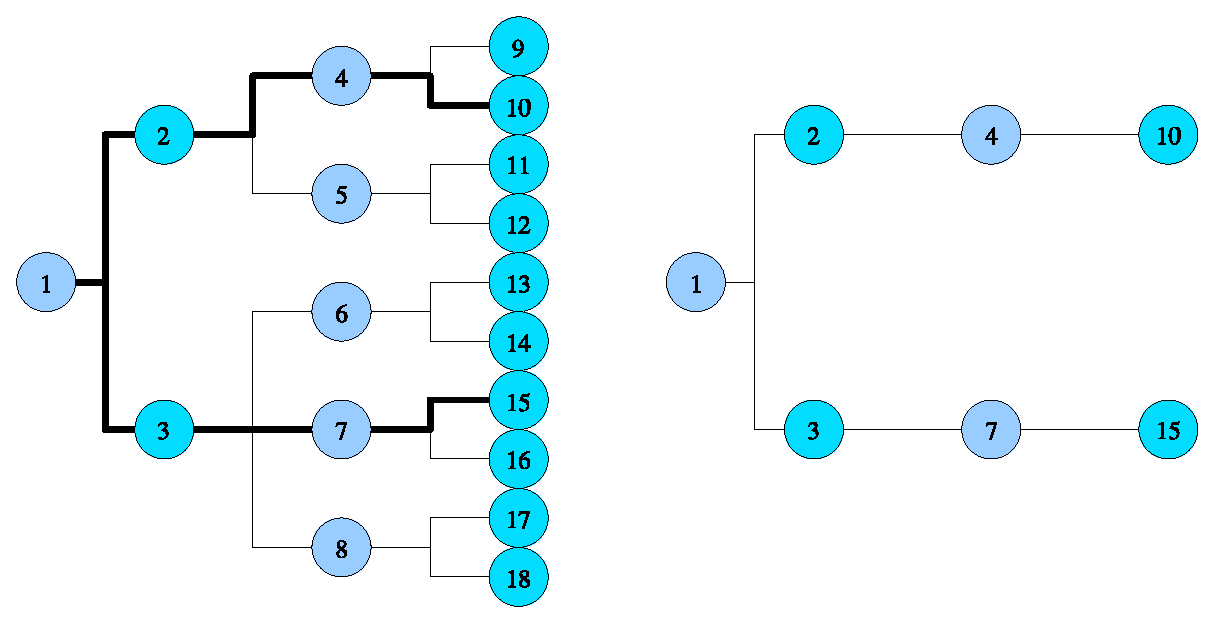
\includegraphics[scale=.6]{figures/redtree.eps}
    \caption{Complete tree and the reduced tree corresponding to the
             chosen scenarios (in bold).}
    \label{fig:Tree}
  \end{center}
  \vspace{-3ex}
\end{figure}

Each of the chosen nodes in the $k$-th stage now becomes the root of a 
branch of the tree, which we call a subtree. In each subtree we choose 
the scenario that minimises the distance to an average scenario in the 
same subtree.
%
Let $S_t$ be the set of nodes in the subtree $S$ at stage $t$, and 
$|S_t|$ its cardinality. For each stage $t$ within subtree $S$, 
we determine an artificial node $n_t$ by averaging the data 
associated to all nodes at this stage:
\[
n_t = \frac{1}{|S_t|} \sum_{l_t \in S_t} (T^{l_t}, W^{l_t}, h^{l_t}, q^{l_t}),
  \qquad k < t \le T.
\]

We define the average scenario for subtree $S$ as the ordered
set of nodes $s_k = \{ l_k, n_{k+1}, \ldots, n_T \}$.
Therefore, the average scenario $\bar s$ (in the complete tree) 
is obtained by listing the 
nodes from the root of the tree to the root of the subtree $S$, and 
then by appending the average nodes. We define it as
\[
\bar s = \{\, l_1, \ldots, l_k, n_{k+1}, \ldots, n_T \,\},
\]
where $l_t = a(l_{t+1})$ for $t = 1,\ldots, k-1$.
Scenario $\bar{s}$ is completely artificial, and there is no guarantee 
that it is feasible: therefore we cannot use it directly as our 
representative scenario. Instead, we use it as a reference point to 
which compare all other scenarios, and thus find the closest scenario 
among the existing ones: this way we do not introduce spurious 
infeasibilities. Hence, in the subtree $S$ we choose the 
representative scenario $s^*$ as 
%
\be  \label{repScenario}
   s^* = s_k, \quad k = \arg\min_{i\in S} \{ (1-p^i) D(s_i, \bar{s}) \},
\ee
%
where, since our ultimate goal is to find the most representative scenario in 
the subtree, we use the term $(1-p^i)$ to ``bring closer'' scenarios 
that have a higher probability of occurring.

The reduced tree selection induces a function $r: \Ctree \to \Rtree$ 
that maps each node of the complete tree to a corresponding node 
in the reduced tree in the following way: if $i \in \Rtree$, then
$r(i) = i$; if $i\not\in \Rtree$, then we choose as $r(i)$ the node in 
the representative scenario corresponding to node $i$ belonging to the
same stage $t$ as node $i$. In other words, to get from node
$i\in\Ctree$ to $r(i)\in\Rtree$ we walk up the tree $\Ctree$ until we
find a node that is also in $\Rtree$, and from there walk back down
the reduced tree until we arrive at the same stage as the original node
This mapping is used to decide how to initialise 
the warm-start iterate for the complete tree, as presented in the
next section. We remark that our generation process guarantees
that for each $i \in \Ctree$, the following properties hold:
\be  \label{eq:ReducedTreeProperties}
  a(r(i)) \in \Rtree, \quad \mbox{ and } \quad a(r(i)) = r(a(i)),
\ee
that is if a node is in the reduced tree so is its parent, and the
mapping $r(\cdot)$ preserves the parent-child relationship. 

Continuing the example started above, we consider two subsets of 
scenarios, corresponding to nodes 9--12 (for the subtree rooted at 
node 2) and to nodes 13--18 (for the subtree rooted at node 3). Within 
each subset we build the scenario of average nodes and then find the 
representative scenario.
The resulting reduced tree is shown in the right of Figure~\ref{fig:Tree}.

We introduce the set $\mathcal{I}_l$ of nodes in the complete tree 
that are initialised by a given node $l\in\Rtree$, that is
$\mathcal{I}_l = \{\, i \in \Ctree : r(i) = l \,\}$, $l \in \Rtree$.
It should be noted that the reduced-tree generation process can be
interpreted as a node-aggregation process: all nodes in
$\mathcal{I}_l\subset\Ctree$ are aggregated into a single node $l\in\Rtree$.
The node aggregation determines the node probabilities $p_R^l$ associated
with each node $l\in\Rtree$; we use:
\be  \label{eq:UpdatePathProbs}
  p^l_R = \sum_{i \in \mathcal{I}_l} p^i.
\ee
Here and in the following we use the convention that symbols referring
to the reduced tree (such as $\Rtree$, $p_R^i$) carry the subscript $_R$.
As will be seen later it is advantageous if the aggregation of nodes
is balanced throughout the tree. On average every node in the reduced
tree corresponds to $n/n_R$ nodes in the full tree, so for
a totally balanced aggregation we would expect 
\[
  \frac{p^i}{p_R^{r(i)}}\frac{n}{n_R}\approx 1.
\]
We define the deviation from this as
\be  \label{eq:rho}
  \rho = \min_{i\in\Rtree}\left\{\frac{p^i}{p_R^{r(i)}}\frac{n}{n_R}, 
                                 \frac{p_R^{r(i)}}{p^i}\frac{n_R}{n}\right\}.
\ee

It is worth noting the effect of the probabilities update
(\ref{eq:UpdatePathProbs}) on the conditional probabilities.
Denote by $\delta^i = p^i/p^{a(i)}$ the conditional probability of
reaching node $i$, given that its parent $a(i)$ has already been
reached.
The conditional probabilities in the reduced tree update according to
\be  \label{eq:UpdateCondProbs}
  \delta_R^l = \!\!\! \sum_{i \in \mathcal{I}_l\cap D_{a(l)}} \!\!\! \delta^i,
  \quad l \in \Rtree.
\ee
To see that \eqref{eq:UpdateCondProbs} holds, we note that for a node $l$
in the $k$-th stage where the subtree selection takes place we have
$\mathcal{I}_l \cap \mathcal{D}_{a(l)} = \mathcal{I}_l$, and
\eqref{eq:UpdateCondProbs} follows from \eqref{eq:UpdatePathProbs}
by dividing through by $p^{a(l)}$.
For a node $l$ after stage $k$ we have $\delta_R^l = 1$, we need to sum
only over the descendants of $a(l)$.
With our reduced-tree selection strategy, for such nodes we actually
have $\delta_R^l = 1$, since there is only one representative scenario
in each subtree.

%
%
\subsection{Construction of the warm-start iterate}
\label{sec:Construction}

Consider the linear programming problem in standard form
\be  \label{eq:CompleteProblem}
  \min\; c^T x \;\qquad \mbox{s.t. }\; Ax = b, \;\; x \ge 0,
\ee
where $A \in \R^{m \times n}$ is full rank, 
$x, c \in \R^{n}$ and $b \in \R^{m}$. 
Problem (\ref{eq:CompleteProblem})
corresponds to the deterministic equivalent \eqref{DetEquiv} generated from a
given event tree $\Ctree$. We will refer to it as the 
{\em complete problem}.

From the reduced tree, which we denote by $\Rtree$, 
we build the reduced deterministic 
equivalent problem
\be \label{eq:ReducedProblem}
\min\; c_R^T x_R \;\quad \mbox{s.t. }\; A_R x_R = b_R, \; x_R \ge 0,
\ee
with $A_R \in \R^{m_R\times n_R}$, $x_R \in 
\R^{n_R}$ and $b_R \in \R^{m_R}$. 
We call problem \eqref{eq:ReducedProblem} the {\em reduced problem}.
As we expect that $(n_R, m_R) \ll (n, m)$, the reduced problem is 
much smaller than the complete formulation, and hence much easier to solve.

We solve problem (\ref{eq:ReducedProblem}) with an interior point method. 
For the reasons presented in Section~\ref{sec:WarmStart}, we do not 
aim for optimality, but instead we aim for a sufficiently advanced 
primal--dual feasible point. Therefore we stop at an iterate
$(x_R^*,y_R^*,s_R^*)\in\mathcal{N}_s(\gamma)$ for a
barrier parameter corresponding to merely few digits of accuracy 
in the solution.
This iterate is used to construct the warm-start point
$(\hat{x}, \hat{y}, \hat{s})$ for the complete problem.

In our approach, the size of the problem changes in both 
the number of constraints and the number of variables.
Therefore, we are faced with the challenge of using 
the reduced-tree solution to provide a warm-start iterate for 
the complete system.
This objective can be achieved on a node by node basis 
by exploiting the inherent structure of the problem.
The sections of the vectors
$\hat{x}, \hat{y}, \hat{s}$ correspoding to node $i\in\Ctree$ are
initialised from the sections of the vectors 
$x_R^*,y_R^*,s_R^*$ correspoding to node $r(i)\in\Rtree$. This process
will be detailed below.

Denote by $\hat x^{i}, \hat y^{i}, \hat s^{i}$ the part of the vectors
$\hat{x}, \hat{y}, \hat{s}$ corresponding to node $i\in\Ctree$ and likewise
$x_R^{i}, y_R^{i},  s_R^{i}$ for components of the solution of the
reduced problem. Then we construct the starting point for the complete
problem in the following manner:
\be  \label{eq:WarmstartSolution}
  \hat x^{i} = x_R^{r(i)}, \qquad 
 (\hat y^{i}, \hat s^{i}) = \frac{p^{i}}{p_R^{r(i)}} (y_R^{r(i)}, s_R^{r(i)}),
  \qquad i \in \Ctree,
\ee
where $p^i_R$ is computed according to (\ref{eq:UpdatePathProbs}).
This means that the dual reduced-tree solution is spread among the
nodes it initialises, as can be seen here:
\[
   \sum_{i \in \mathcal{I}_k} (\hat y^i, \hat s^i)
  = \sum_{i \in \mathcal{I}_k} \frac{p^i}{p^k_R} (y^k_R, s^k_R)
  = (y^k_R, s^k_R) \frac{1}{p^k_R} \sum_{i \in \mathcal{I}_k} p^i 
  = (y^k_R, s^k_R), \qquad k \in \Rtree.
\]

Considering again the example of Figure~\ref{fig:Tree}, suppose that 
in the reduced tree we accepted only the scenarios that end at 
node 10 and node 15, so that the reduced tree consists of nodes 
1, 2, 3, 4, 7, 10 and 15. By solving the corresponding reduced problem, 
we obtain the parts of the solution vector associated to such 
nodes: these can be used directly in the complete iterate
(Figure~\ref{fig:Solution} top). 
We fill the missing elements 
by reproducing the solution from the nodes in the same subtree 
and the same stage (Figure~\ref{fig:Solution} bottom).
The proposed way of constructing the complete iterate is easy to
implement and its execution time is negligible.
%
\begin{figure}[ht]
  \begin{center}
    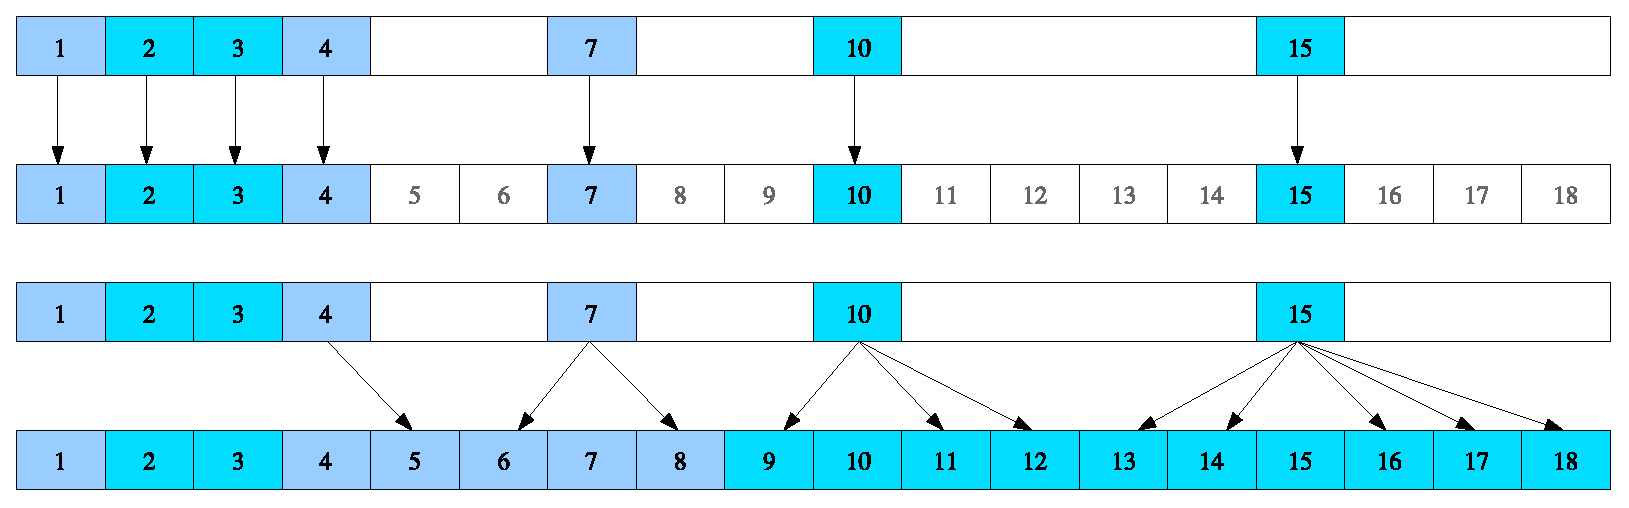
\includegraphics[scale=.51]{figures/solution.eps}
    \caption{Generation of the warm-start iterate.}
    \label{fig:Solution}
  \end{center}
  \vspace{-3ex}
\end{figure}

\ignore{
This simple strategies can be further 
generalised by considering a linear combination of the solutions 
corresponding to nodes that belong to the same stage. In this sense, 
the parts of the solution for nodes 4 and 7 may be used to initialise 
the solution for nodes 5, 6 and 8 (similarly for nodes 10 and 15 to 
initialise the starting solution for the other leaf nodes).
}

%
% Section
%
\section{Analysis of the warm-start iterate}
\label{sec:Analysis}

In this section we study how the warm-start iterate generated with 
the procedures presented above satisfies the conditions expressed by 
Gondzio and Grothey \cite{GondzioGrothey03}. 
Contrary to what is assumed in both \cite{YildirimWright} and 
\cite{GondzioGrothey03}, in our approach the dimension of the problem changes, 
as the reduced tree problem is, by construction, much smaller than the 
complete problem.

However, in a similar way as we did with the solution vector, 
we can expand the reduced problem to one which has the same dimension 
as the complete problem (\ref{eq:CompleteProblem}) by replicating
the blocks in the coefficient matrix and in the objective and right-hand 
side vectors, as shown in Figure~\ref{fig:ExpandedSystem}.
%
\begin{figure}[ht]
  \begin{center}
    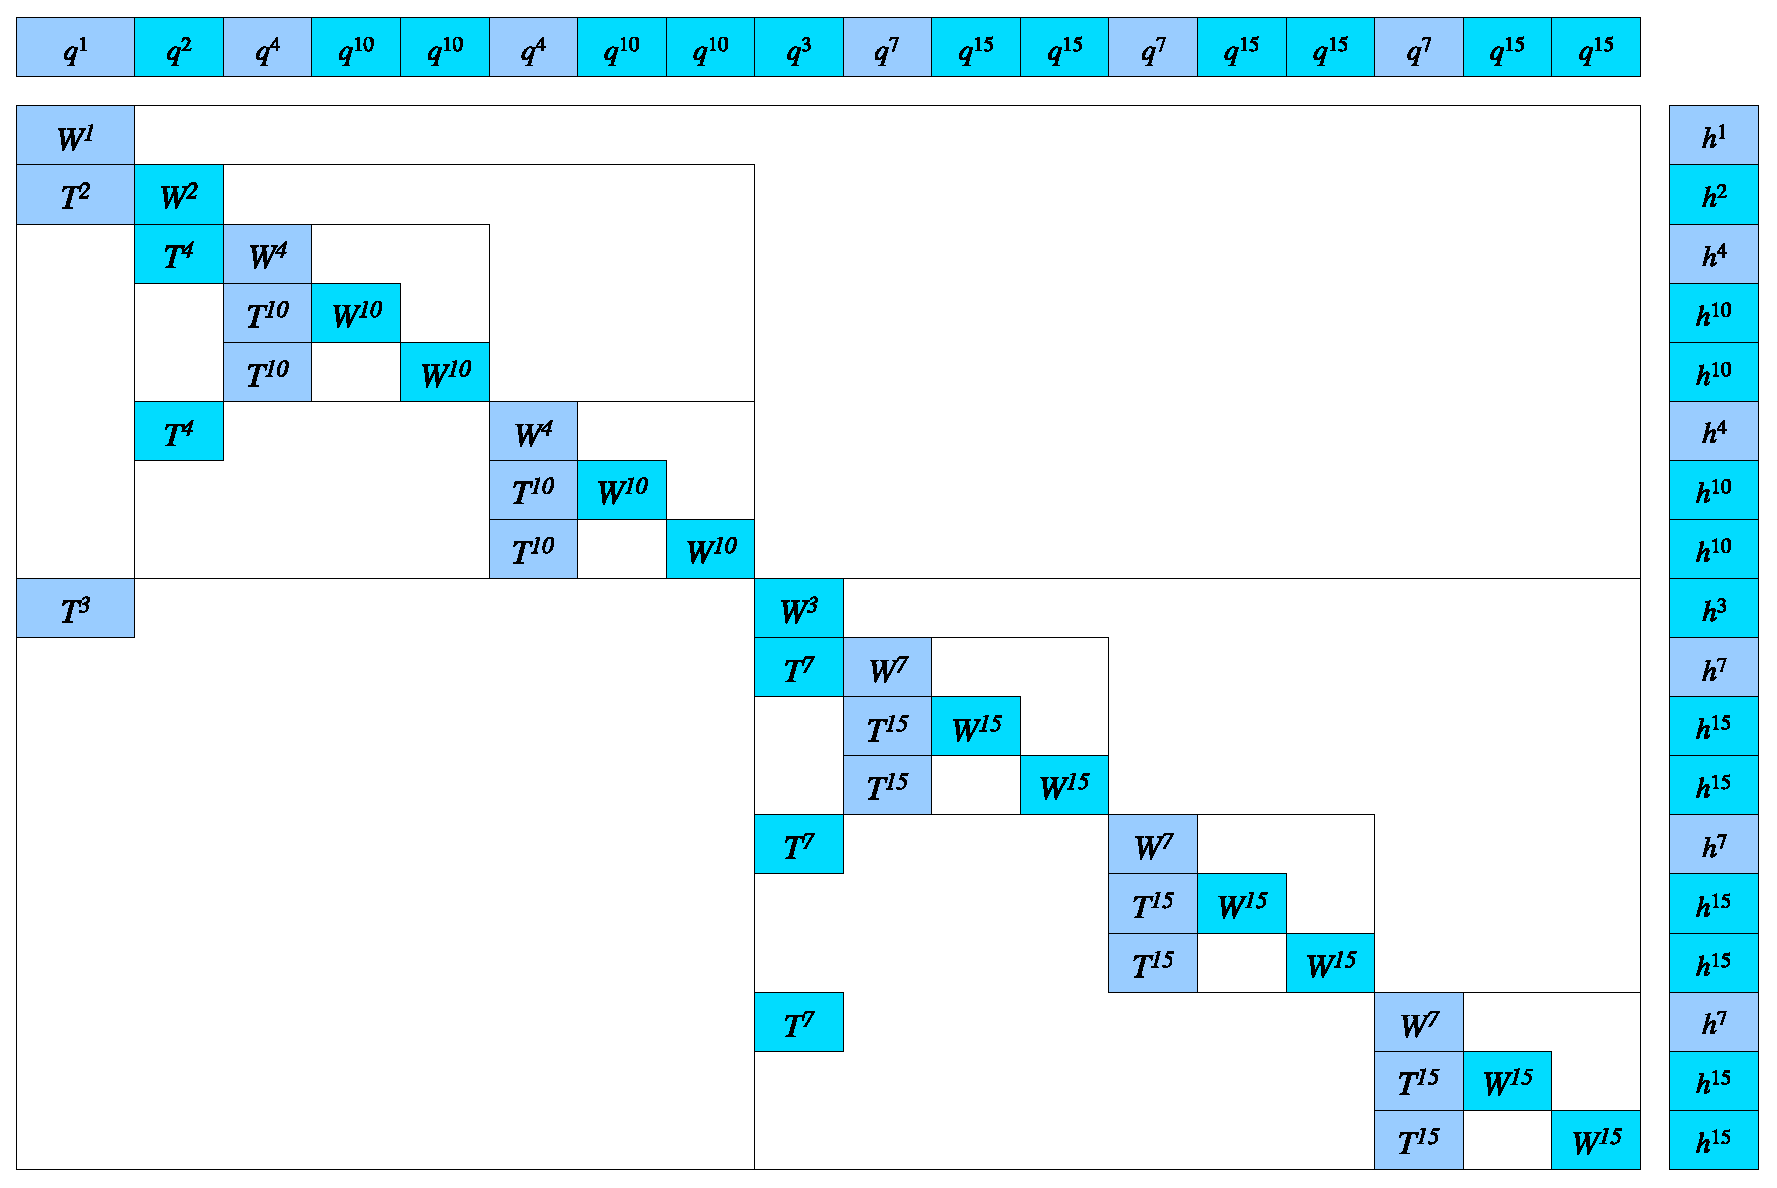
\includegraphics[scale=.50]{figures/expandedsystem.eps}
    \caption{The expanded system for the event tree of Figure~\ref{fig:Tree}.}
    \label{fig:ExpandedSystem}
  \end{center}
  \vspace{-3ex}
\end{figure}

This corresponds to creating the (artificial) {\em expanded problem}
\be \label{eq:ExpandedProblem}
\min\; \hat{c}^T x \;\quad \mbox{s.t. }\; \hat{A} x = \hat{b},
    \; x \ge 0,
\ee
the dimension of which, $\hat{A} \in \R^{m\times n}$, 
$\hat{c}, x \in \R^{n}$ and $\hat{b} \in \R^{m}$,
corresponds to the dimension of the complete problem 
(\ref{eq:CompleteProblem}).
Using the notation introduced earlier, we will denote 
all symbols referring to the expanded problem with a hat $\hat{\ }$.

To analyse the warm-start iterate we can now follow a two-step
procedure. First we note that from an advanced iterate 
$(x_R, y_R,  s_R)\in\mathcal{N}^R_s(\gamma)$ for the reduced
problem the procedure in (\ref{eq:WarmstartSolution}) constructs a
primal--dual feasible point $(\hat{x}, \hat{y}, \hat{s})$ for the 
expanded problem. Indeed we will show 
$(\hat{x}, \hat{y}, \hat{s})\in\hat{\mathcal{N}}_s(\hat{\gamma})$
in Theorem~\ref{th:NeighbourhoodExpandedSolution}. In the second step we
can use this iterate to warmstart the complete problem. Since in the
step from the expanded to the complete problem only the problem data
changes but not its size, the methods developed in
\cite{GondzioGrothey03,YildirimWright} can be used to analyse the 
warm-start iterate.

We start the analysis with a technical result.

\begin{lemma}  \label{th:SumOfTerms}
Let $l\in\Ctree$, then
\[
\sum_{i \in \mathcal{D}_{l}} {T^{r(i)}}^T \hat y^i
  = \frac{p^{l}}{p^{r(l)}_R}\sum_{k \in \mathcal{D}_{r(l)}^R}
    {T^k}^T y^k_R.
\]
\end{lemma}
%
\begin{proof}
We have this chain of identities:
\[
\begin{split}
\sum_{i \in \mathcal{D}_{l}} {T^{r(i)}}^T \hat y^i
  &= \sum_{i\in\mathcal{D}_{l}} {T^{r(i)}}^T y^{r(i)}_R\frac{p^i}{p^{r(i)}_R}\\
  &= \frac{p^{l}}{p^{r(l)}_R}\sum_{i \in \mathcal{D}_{l}} {T^{r(i)}}^T
    y^{r(i)}_R \frac{\delta^i}{\delta_R^{r(i)}}\\
  &= \frac{p^{l}}{p^{r(l)}_R}\! \sum_{k \in \mathcal{D}_{r(l)}^R} \!\!
       \frac{{T^k}^T y^k_R}{\delta_R^k}
       \sum_{i \in \mathcal{I}_k \cap \mathcal{D}_{l}}\!\!\! \delta^{i},
\end{split}
\]
where the second equal sign follows from $p^i = p^l\delta^i$ and
$p_R^{r(i)} = p_R^{r(l)}\delta_R^{r(i)}$ for $i \in \mathcal{D}_l$. 
The last equality follows from the fact that we can partition
$\mathcal{D}_l$ according to which nodes of the reduced tree are used
for initilisation:
\(
  \mathcal{D}_{l} = \bigcup_{k \in \mathcal{D}_{r(l)}^R}
     \mathcal{I}_{k} \cap \mathcal{D}_{l}.
\)
The claim then follows from (\ref{eq:UpdateCondProbs}).
\end{proof}

\begin{theorem}  \label{th:FeasibleExpandedSolution}
If $(x_R, y_R, s_R)$ is primal and dual feasible for
the reduced problem (\ref{eq:ReducedProblem}),
then the warm-start solution $(\hat{x}, \hat{y}, \hat{s})$
obtained from (\ref{eq:WarmstartSolution}) is 
primal and dual feasible for the expanded problem (\ref{eq:ExpandedProblem}).
\end{theorem}
%
\begin{proof}
As $\hat x^{l} = x^{r(l)}_R$, primal feasibility is trivially
satisfied:
\be  \label{eq:RedTreePrimalContribution}
   T^{r(l)}\hat x^{a(l)} + W^{r(l)} \hat x^{l} =  h^{r(l)}, 
      \qquad l \in \Ctree.
\ee
%
Now we consider dual feasibility. 
By assumption, the reduced problem solution satisfies 
the dual constraints:
\[
  {W^{r(l)}}^T y^{r(l)}_R +\sum_{i \in \mathcal{D}^R_{r(l)}} {T^{r(i)}}^T
     y^{r(i)}_R + s^{r(l)}_R = p^{r(l)}_R q^{r(l)},
     \qquad r(l) \in \Rtree.
\]
Multiplying both terms by $p^{l}/p^{r(l)}_R$ we obtain
\[
  \frac{p^{l}}{p^{r(l)}_R} \Big( {W^{r(l)}}^T y^{r(l)}_R
     +\sum_{i\in \mathcal{D}_{r(l)}^R} {T^{r(i)}}^T y^{r(i)}_R + s^{r(l)}_R
     \Big) = p^{l} q^{r(l)},
\]
which, according to (\ref{eq:WarmstartSolution}) and 
Lemma~\ref{th:SumOfTerms}, becomes
\be  \label{eq:RedTreeDualContribution}
  {W^{r(l)}}^T \hat y^{l}+\sum_{i\in\mathcal{D}_{l}}{T^{r(i)}}^T \hat y^i
   + \hat s^{l} = p^{l} q^{r(l)}, \qquad l \in \Ctree,
\ee
so $(\hat y, \hat s)$ satisfies
the dual constraints in the expanded problem.
\end{proof}

\begin{theorem}  \label{th:NeighbourhoodExpandedSolution}
If $(x_R, y_R, s_R) \in \mathcal{N}^R_s(\gamma)$ 
for some $\gamma\in(0,1)$, then $(\hat{x}, \hat{y}, \hat{s})\in
\widehat{\mathcal{N}}_s(\rho\gamma)$,
with $\rho$ defined in (\ref{eq:rho}).
\end{theorem}
%
\begin{proof}
From Theorem~\ref{th:FeasibleExpandedSolution}, the warm-start iterate 
$(\hat x, \hat y, \hat s)$ is feasible in the reduced system.
Hence, here we only need to prove centrality. 
We observe that 
\begin{eqnarray*}
  \hat{\mu} &=& \frac{\hat{x}^T\hat{s}}{n} 
   = \frac{1}{n}\sum_{i \in \Ctree}(\hat x^i)^T\hat{s}^i 
   = \frac{1}{n}\sum_{k\in \Rtree}\sum_{i\in I_k} (\hat{x}^i)^T\hat{s}^i \\
  &=& \frac{1}{n}\sum_{k\in \Rtree}\sum_{i\in I_k} \frac{p^i}{p_R^k} 
      (x_R^k)^T s_R^k \\
  &=& \frac{1}{n} \sum_{k\in\Rtree} \frac{1}{p_R^k}(x_R^k)^T s_R^k
      \sum_{i\in I_k}p^i\\
  &=& \frac{n_R}{n} \mu_R,
\end{eqnarray*}
where we used (\ref{eq:WarmstartSolution}) and (\ref{eq:UpdatePathProbs}), 
and $\mu_R = x_R^Ts_R/n_R$. 
Hence, since $(x_R, y_R, s_R)\in N_s(\gamma)$ 
implies $(x_R)_j (s_R)_j\ge \gamma\mu_R$, for $j = 1, \ldots, n_R$, 
and using (\ref{eq:rho}) we have
\[
  \hat x^l_j\hat s^l_j = (x_R^{r(l)})_j (s_R^{r(l)})_j
                         \frac{p^l}{p_R^{r(l)}}
                       \ge \gamma\mu_R \frac{p^l}{p_R^{r(l)}}
		       = \gamma\hat\mu \frac{n}{n_R}\frac{p^l}{p_R^{r(l)}}
                       \ge \rho\gamma\hat{\mu},
		       \qquad l \in \Ctree.
\]
The upper bound $\hat x^l_j\hat s^l_j\le \hat{\mu}/(\rho\gamma)$
can be derived similarly.
\end{proof}

%
%
\subsection{Absorbing perturbations}

We argue that the difference between the data of the expanded 
problem (\ref{eq:ExpandedProblem}) and that of the original (complete) 
problem (\ref{eq:CompleteProblem}) can be interpreted as a perturbation 
between two problem instances of identical dimension. 
Clearly the expanded system has merely a theoretical
interest, as we use it to evaluate the magnitude of the 
perturbation introduced, and we never generate it in practice.

We assume that a feasible long-step path-following algorithm based on
the symmetric neighbourhood $\Nhood_s(\gamma)$ 
is used to solve the warmstarted complete problem. 
Although the constructed warm-start iterate $(\hat{x}, \hat{y}, \hat{s})$ 
from (\ref{eq:WarmstartSolution}) is feasible in the expanded problem, 
it is not feasible in the complete problem. 
As in \cite{YildirimWright} and \cite{GondzioGrothey03} we derive
conditions that guarantee to absorb these infeasibilities with one
{\em modification step}. 
For this consider the following Newton system:
\be \label{eq:NewtonSystem2}
\left[ \begin{array}{ccc}
    A & 0 & 0 \\ 0 &A^T & I \\ \hat{S} & 0 & \hat{X}
  \end{array} \right]
\left[ \begin{array}{c}
    \Delta x \\ \Delta y \\ \Delta s
  \end{array} \right] = 
\left[ \begin{array}{c}
    \xi_b \\ \xi_c \\ 0
  \end{array} \right],
\ee
where $\xi_b = b - A\hat{x}$ and $\xi_c = c - A^T\hat{y}+\hat{s}$ are the
infeasibilities incurred by using the expanded iterate $(\hat{x},
\hat{y}, \hat{s})$ to warmstart the complete problem. 
Such a modification is termed a {\em Newton step correction} in
\cite{YildirimWright} or an {\em Additional centering iteration}
in \cite{GondzioGrothey06}. 
Gondzio and Grothey \cite{GondzioGrothey03} analyse the
same system, but are concerned with absorbing primal and dual
infeasibility separately by splitting (\ref{eq:NewtonSystem2}) into
two separate directions.
We will give a more general result and apply it to the situation of
warm start for stochastic programming problems. To avoid overburdening
notation we will drop the hat from the warm-start vectors.
We will keep it in the neighbourhoods to make a clear distinction between
$\widehat{\mathcal{N}}_s(\gamma)$ and $\mathcal{N}_s(\gamma)$
denoting the symmetric neighbourhoods 
for the expanded problem \eqref{eq:ExpandedProblem}
and the complete problem \eqref{eq:CompleteProblem}, respectively.

After some straightforward manipulation following the arguments of 
\cite{GondzioGrothey03}, the Newton
direction (\ref{eq:NewtonSystem2}) can be expressed in terms 
of the primal and dual residuals $\xi_b$, $\xi_c$ as
%
\begin{eqnarray}  \label{eq:Directions}
  \Delta x & \hspace{-1ex} = \hspace{-1ex} & 
  (XS^{-1} \! A^T (AXS^{-1} \!\! A^T)^{-1} \! AXS^{-1} \!\!-\!\! XS^{-1} )\xi_c
  \! + \! XS^{-1} \! A^T (AXS^{-1} \! A^T)^{-1} \xi_b, \nonumber \\
  \Delta y & \hspace{-1ex} = \hspace{-1ex} & 
  (AXS^{-1} A^T)^{-1} (AXS^{-1} \xi_c + \xi_b),                  \\
  \Delta s & \hspace{-1ex} = \hspace{-1ex} & 
  (I - A^T (AXS^{-1} \! A^T)^{-1} AXS^{-1} )\xi_c 
  \! - \! A^T (AXS^{-1} \! A^T)^{-1} \xi_b.            \nonumber
\end{eqnarray}

We consider the matrix
\[
  Q = I - S^{-1} A^T (A X S^{-1} A^T)^{-1} A X,
\]
and restate Lemma~3.2 of \cite{GondzioGrothey03},
which provides a bound on the norm of $Q$, in terms of
the symmetric neighbourhood $N_s(\gamma)$.

\begin{lemma}  \label{th:BoundQ}
If $w \in \Nhood_s(\gamma)$, then $\|Q\|_2 \le 1/\gamma$.
\end{lemma}
%
\begin{proof}
For a point $w \in \Nhood_s(\gamma)$, 
the following inequalities hold:
\[
  (x_i s_i)^{-1/2} \le (\gamma\mu)^{-1/2},
  \quad \mbox{ and } \quad
  (x_i s_i)^{1/2} \le (\mu / \gamma)^{1/2}.
\]
With some manipulations, we can express matrix $Q$ as
\[
Q = X^{-1/2}S^{-1/2} \left[ I - X^{1/2}S^{-1/2}A^T(AXS^{-1}A^T)^{-1}AX^{1/2}S^{-1/2} \right] X^{1/2}S^{1/2},
\]
where the term in square brackets is an orthogonal projection on the null
space of $AX^{1/2}S^{-1/2}$, so its Euclidean norm is 1.
As desired, we obtain
\[
  \| Q \|_2 = \| X^{-1/2}S^{-1/2} \|_2 \| X^{1/2}S^{1/2} \|_2 \le 1/\gamma.
  \qedhere
\]
\end{proof}

In the next Lemma we state sufficient conditions for the perturbations
to guarantee a full Newton step.

\begin{lemma}  \label{th:FullNewtonStep}
Let $w \in \widehat{\Nhood}_s(\gamma)$ be the warm-start iterate 
and define the scaled residuals 
\be  \label{eq:ScaledResiduals}
  \tilde \xi_b = X^{-1} A^T (A A^T)^{-1} \xi_b 
  \quad \mbox{ and } \quad 
  \tilde \xi_c = S^{-1} \xi_c.
\ee
If for $\beta < 1$ we have
\[
\|\tilde{\xi}_b\|_\infty + \|\tilde{\xi}_c\|_\infty 
    \le \beta\left(1 + \sqrt{n} / \gamma \right)^{-1},
\]
then the full Newton step (\ref{eq:NewtonSystem2}) from 
the warm-start iterate can be taken and absorbs the complete infeasibilities.
\end{lemma}
%
\begin{proof}
Using the definitions of the matrix $Q$ and of the relative residual 
vectors (\ref{eq:ScaledResiduals}),
the relations (\ref{eq:Directions}) simplify to
\[
   X^{-1}\Delta x = -Q \tilde{\xi}_c + (I-Q) \tilde{\xi}_b = -S^{-1}\Delta s,
\]
%\begin{eqnarray*}
%   X^{-1}\Delta x & \!\! = \!\! & 
%       -Q \tilde{\xi}_c + (I-Q) \tilde{\xi}_b, \\
%   S^{-1}\Delta s & \!\! = \!\! & 
%        Q \tilde{\xi}_c - (I-Q) \tilde{\xi}_b, 
%\end{eqnarray*}
%
yielding the bound
%
\be  \label{boundx}
\|X^{-1}\Delta x\|_\infty
  \le \|Q\|_\infty\|\tilde{\xi}_c\|_\infty 
       + (1 + \|Q\|_\infty)\|\tilde{\xi}_b\|_\infty
  \le (1 +\|Q\|_\infty)(\|\tilde{\xi}_b\|_\infty + \|\tilde{\xi}_c\|_\infty).
\ee
%
As $(x,y,s)\in \widehat{\Nhood}_s(\gamma)$, using Lemma~\ref{th:BoundQ} we get
that $\|Q\|_\infty \le \sqrt{n} \|Q\|_2 \le \sqrt{n} / \gamma$.
Substituting it into (\ref{boundx}), we obtain
\[
\|X^{-1}\Delta x\|_\infty
   \le \left(1+\sqrt{n} / \gamma \right)(\|\tilde{\xi}_b\|_\infty 
       + \|\tilde{\xi}_c\|_\infty),
\]
which, under the condition of the Lemma, implies 
\begin{equation}  \label{eq:FullNewtonStep}
\|X^{-1}\Delta x\|_\infty = \|S^{-1}\Delta s\|_\infty \le \beta,
\end{equation}
that is the full Newton step is feasible, as $\beta < 1$.
\end{proof}

\begin{theorem}
Let $w \in \widehat\Nhood_s(\gamma)$ and $\beta < 1$.
Under the conditions of Lemma~\ref{th:FullNewtonStep},
%The full Newton step in the direction $(\Delta x, \Delta y, \Delta s)$
%is feasible and 
the new point
$\tilde w = (x + \Delta x, y + \Delta y, s + \Delta s)
\in \mathcal{N}_s(\frac{1-\beta^2}{1+\beta^2}\gamma)$.
\end{theorem}

\begin{proof}
At the new point $\tilde w$ the barrier parameter is
\be  \label{eq:NewBarrier}
  n \tilde\mu = \sum_{i=1}^n \tilde x_i \tilde s_i 
              = \sum_{i=1}^n (x_i +\Delta x_i)(s_i +\Delta s_i)
              = \sum_{i=1}^n (x_is_i + \Delta x_i\Delta s_i),
\ee
as the last equation of (\ref{eq:NewtonSystem2}) implies
$s_i\Delta x_i + x_i\Delta s_i = 0$, $i = 1, \ldots, n$.
%
Using (\ref{eq:FullNewtonStep}) from Lemma~\ref{th:FullNewtonStep}, 
we have that
$\|X^{-1}\Delta x\|_\infty\|S^{-1}\Delta s\|_\infty \le \beta^2$,
and so
\be  \label{eq:BoundsDeltaxDeltas}
 -\beta^2x_i s_i \le \Delta x_i \Delta s_i \le \beta^2 x_i s_i;
\ee
by summing up all products we obtain
\[
 -\beta^2 n\mu \le \sum_{i=1}^n \Delta x_i \Delta s_i \le \beta^2 n\mu,
\]
which, by adding $n\mu = \sum_i x_i s_i$ to all terms and using 
(\ref{eq:NewBarrier}), leads to
\be  \label{eq:BoundsNewBarrier}
  (1-\beta^2) n\mu \le n \tilde \mu \le (1+\beta^2) n\mu.
\ee

We now study whether the new iterate is still in (some) symmetric
neighbourhood of the central path by checking the pairwise
complementary products
\[
\tilde x_i \tilde s_i = x_is_i + \Delta x_i\Delta s_i
                      = \Big(1 +\frac{\Delta x_i\Delta s_i}{x_is_i}\Big)x_is_i.
\]
Using (\ref{eq:BoundsDeltaxDeltas}) and (\ref{eq:BoundsNewBarrier}) 
we obtain
\begin{eqnarray*}
\tilde x_i \tilde s_i \ge (1-\beta^2)\gamma\mu 
                      \ge \frac{1-\beta^2}{1+\beta^2}\gamma\tilde\mu, \\
\tilde x_i \tilde s_i \le (1+\beta^2)\frac{\mu}{\gamma} 
                      \le \frac{1+\beta^2}{1-\beta^2}\frac{1}{\gamma}\tilde\mu,
\end{eqnarray*}
which proves the statement of the theorem.
\end{proof}

%
%
\subsection{Conditions on the warm-start iterate}

We use Lemma~\ref{th:FullNewtonStep} to obtain conditions that the 
reduced tree has to satisfy in order for a warm start of the complete problem 
to be successful. In order to prove this result, we need to assume that 
the primal--dual solution $(x_R^\ast, y_R^\ast, s_R^\ast)$ to the reduced 
stochastic programming problem is uniformly bounded, say,
%
\be  \label{xysBound}
  \max\{\|x_R^\ast\|_\infty, \|y_R^\ast\|_\infty, \|s_R^\ast\|_\infty\} \le B,
  \quad
  \max\{\|(X_R^\ast)^{-1}e\|_\infty,\|(S_R^\ast)^{-1}e\|_\infty\} \le B,
\ee
%
where $B>1$. 
It is worth noting that since we work with the symmetric neighbourhood
(\ref{eq:SymmetricNeighbourhood}), 
we actually need only the first inequality to hold.
Indeed, if $x_j^\ast \leq B$ then 
$1 / s_j^\ast \leq x_j^\ast / (\gamma \mu) \leq B / (\gamma \mu)$
and, similarly, if $s_j^\ast \leq B$ then 
$1 / x_j^\ast \leq s_j^\ast / (\gamma \mu) \leq B / (\gamma \mu)$.
In other words, the boundedness of the iterate 
$(x_R^\ast, y_R^\ast, s_R^\ast)$ implies the boundedness of the 
component-wise inverses of $x_R^\ast$ and $s_R^\ast$.

\ignore{
We argue that our way of constructing a reduced event tree by choosing
scenarios that minimize the distance from a representative average
scenario from each subtree can be designed to produce perturbations
which satisfy the assumptions of Lemma~\ref{th:FullNewtonStep}.
}

The reduced problem solution is in a neighbourhood of the central path 
for the reduced problem. In particular, this is the case if additional 
centering steps are computed once the desired tolerance level has been 
attained \cite{Gondzio98}. 
Using the feasibility result of Theorem~\ref{th:FeasibleExpandedSolution},
the residuals for the complete problem at the warm-start point 
$(\hat{x}, \hat{y}, \hat{s})$ are:
\[
\begin{array}{rll}
  \xi_b \!\!&=\; b-A\hat x           \!\!&=\: (b-\hat b)-(A-\hat A)\hat x,  \\
  \xi_c \!\!&=\; c -A^T\hat y-\hat s \!\!&=\: (c-\hat c)-(A-\hat A)^T\hat y.\\ 
\end{array}
\]
%
It is crucial to ensure that the primal and dual residuals 
$\xi_b$ and $\xi_c$ are small. 
By construction, the elements of the vectors 
$(b-\hat{b})$ and $(c-\hat{c})$ that correspond to nodes in the reduced 
tree are zero; for the same reason, the corresponding blocks of 
$(A-\hat{A})$ are zero as well.
%
The elements corresponding to the nodes not considered in the reduced 
tree will be, in general, non zero. However, as the scenarios 
in the reduced tree were chosen according to (\ref{repScenario}) 
in order to minimize the distance 
from the average case, we expect the perturbations to be small. 

We can now state the following result, in which we obtain some bounds
on the size of the primal and dual perturbations.
%
\begin{lemma}  \label{th:BoundResiduals}
Let the reduced tree be chosen in such a way that for every node 
$i \in \Ctree$ the node distance (\ref{eq:Distance}) is 
$d(r(i), i) < \varepsilon$, for an $\varepsilon > 0$.
If the reduced problem solution is primal and dual feasible  
and satisfies (\ref{xysBound}), then
$\| \xi_b \|_{\infty} \leq \varepsilon B$
and  $\| \xi_c \|_{\infty} \leq \varepsilon B|\Rtree|$, where
$|\Rtree|$ is the number of nodes in the reduced tree.
\end{lemma} 
%
\begin{proof}
Using the form of the stochastic programming problem (\ref{DetEquiv})
we can write the primal residual of the complete problem as
\[
  \|\xi_b\|_\infty = \|b-A\hat x\|_\infty 
                   = \max\{\|h^{l} - T^{l}\hat x^{a(l)} 
                     - W^{l}\hat x^{l}\|_\infty:l = 1,\ldots,L_T\}.
\]
%
The contribution of a node $l \in \Ctree$ to $\xi_b$ is 
\[
\begin{split}
  \| \xi_b^{l} \|_{\infty}
    & = \|h^{l}\!-\!T^{l}\hat x^{a(l)}\!-\!W^{l}\hat x^{l}\| \\
    & = \|h^{l} \!-\! h^{r(l)} - (T^{l} \!- T^{r(l)})\hat x^{a(l)}
        - (W^{l} - W^{r(l)}) \hat x^{l}\| \\
%   & \le \|h^{l} \! - \! h^{r(l)}\| +
%         \|T^{l} \! - \! T^{r(l)}\| \| x^{a(r(l))}_R \|
%         + \|W^{l} - W^{r(l)}\| \| x^{r(l)}_R\| \\
    & \le \big( \|h^{l} \! - \! h^{r(l)}\| +
           \|T^{l} \! - \! T^{r(l)}\| +
           \|W^{l} \! - \! W^{r(l)}\| \big) B \\
    & \le  d(l, r(l)) B \le \varepsilon B,
\end{split}
\]
where the step from the first to the second line uses 
(\ref{eq:RedTreePrimalContribution}), and all norms here 
are infinity norms.
%
This clearly implies that $\| \xi_b \|_\infty \le \varepsilon B$. 

The dual residual for the complete problem at the warm-start point 
can be written as
\[
  \|\xi_c\|_\infty = \|c -A^T\hat y -\hat s \|_\infty 
                   = \max\{\|p^{l}q^{l}
                   - {W^{l}}^T\hat y^{l} 
                   - \sum_{i \in \mathcal{D}_{l}} {T^{i}}^T\hat y^{i}
                   - \hat s^{l}
  \|_\infty : l = 1,\ldots,L_T\}.
\]
%
The contribution of a node $l \in \Ctree$ to $\xi_c$ is
\[
\begin{split}
  \xi_c^{l} 
 & = p^{l} q^{l} - {W^{l}}^T\hat y^{l}
     - \sum_{i\in \mathcal{D}_{l}} {T^i}^T \!\hat y^{i} -\hat s^{l} \\
 & = p^{l}(q^{l}\!-\! q^{r(l)})
     - (W^{l} \!-\! W^{r(l)})^T \hat y^{l}
     -\sum_{i \in \mathcal{D}_{l}} (T^{i} \!-\! T^{r(i)})^T\hat y^i \\
% & = p^{l}(q^{l} \!-\! q^{r(l)})
%     - \frac{p^{l}}{p^{r(l)}_R}(W^{l} \!-\! W^{r(l)})^T y^{r(l)}_R
%     -\sum_{i \in \mathcal{D}_{l}} (T^{i} \!-\! T^{r(i)})^T 
%           \frac{p^i}{p^{r(i)}_R} y^{r(i)}_R \\
 & = p^{l}(q^{l} \!-\! q^{r(l)})
     - \frac{p^{l}}{p^{r(l)}_R} \Big[
       (W^{l} \!-\! W^{r(l)})^T y^{r(l)}_R
       +\sum_{i\in \mathcal{D}_{l}} %\setminus\mathcal{D}_{r(l)}^R}
           (T^{i} \!-\! T^{r(i)})^T 
           \frac{\delta^i}{\delta^{r(i)}_R} y^{r(i)}_R \Big],
\end{split}
\]
where the step from the first to the second line uses 
(\ref{eq:RedTreeDualContribution}) and the next step uses
(\ref{eq:WarmstartSolution}) together with $p^i = p^l\delta^i,
p_R^{r(i)} = p_R^{r(l)}\delta_R^{r(i)}$.
% and in the last line we 
%exploited the fact that $T^i - T^{r(i)} = 0$
%for $i \in \mathcal{D}_{l}\cap\mathcal{D}_{r(l)}^R$.
%
Taking norms (all norms here are infinity norms)
and using the partitioning 
$\mathcal{D}_l = \bigcup_{k\in D^R_{r(l)}} \mathcal{I}_k\cap\mathcal{D}_l$
we obtain
\[
\begin{split}
  \| \xi_c^{l} \|_\infty
  & \le \|q^{l} - q^{r(l)}\| 
        + \|W^{l} - W^{r(l)}\| \| y^{r(l)}_R\|
        + \!\!\! \sum_{k\in \mathcal{D}_{r(l)}^R} \!\!\! \| y^{k}_R \| \!\!
          \sum_{i\in \mathcal{I}_k \cap \mathcal{D}_{l}\setminus \{k\} }
	  \!\!\! \| T^{i} - T^{k} \| \frac{\delta^i}{\delta_R^k} \\
  & \le \|q^{l} - q^{r(l)}\| 
        + \|W^{l} - W^{r(l)}\| \| y^{r(l)}_R\|
        + \!\!\! \sum_{k\in \mathcal{D}_{r(l)}^R} \!\!\! \| y^{k}_R \|
          \varepsilon \!\!
          \sum_{i\in \mathcal{I}_k \cap \mathcal{D}_{l}\setminus \{k\} }
	  \! \frac{\delta^i}{\delta_R^k} \\
  & \le \Big( \|q^{l} - q^{r(l)}\| 
        + \|W^{l} - W^{r(l)}\|
        + \!\!\! \sum_{k\in \mathcal{D}_{r(l)}^R} \!\!\!
	  \big( 1 - \frac{\delta^k}{\delta_R^k} \big) \varepsilon \Big) B
    \le \varepsilon B |\Rtree|.
%        \max_{l} |\mathcal{D}_{l}^R| (1 - \frac{\delta^k}{\delta^k_R}).
        \qedhere
\end{split}
\]
%
%This clearly implies that $\| \xi_c \|_\infty \le \varepsilon B$. 
\end{proof}

The following result combines the findings of Lemmas~\ref{th:FullNewtonStep} 
and \ref{th:BoundResiduals}. 
%
\begin{theorem}  \label{th:Final}
Let the assumptions of Lemma~\ref{th:BoundResiduals} be satisfied and 
\[
\varepsilon B^2 \max\{\|A\|_\infty\|(AA^T)^{-1}\|_\infty, \; |\Rtree|\} 
   \le \frac{1}{2} \beta \left(1+\sqrt{n} / \gamma \right)^{-1}.
\]
Then the full Newton step (\ref{eq:NewtonSystem2})
from the warm-start iterate is feasible 
and it restores primal and dual feasibility.
\end{theorem}
%
\begin{proof}
Using the definition of $\tilde{\xi}_b$ from (\ref{eq:ScaledResiduals}),
the bounds (\ref{xysBound}), and Lemma~\ref{th:BoundResiduals}, we get
\[
\| \tilde{\xi}_b \|_{\infty} = \| X^{-1} A^T (AA^T)^{-1} \xi_b \|_{\infty} 
    \le
    \varepsilon B^2 \|A\|_{\infty} \|(AA^T)^{-1}\|_{\infty} 
    \le \frac{1}{2} \beta \left(1+\sqrt{n} / \gamma \right)^{-1},
\]
In a similar way, we obtain
\[
  \| \tilde{\xi}_c \|_{\infty} = \| S^{-1} \xi_c \|_\infty
                  \le \varepsilon B^2 |\Rtree|
                  \le \frac{1}{2} \beta \left(1+\sqrt{n} / \gamma \right)^{-1}.
 \]
Now the result follows from  Lemma~\ref{th:FullNewtonStep}. 
\end{proof}

A few remarks are in order about these results.
Theorem~\ref{th:Final} implies that if we can choose the reduced
scenario tree such that $\varepsilon = \max_i\{d(r(i),i)\}$ is small enough
to satisfy the bound given in the Theorem, then the warm-start point
constructed from the reduced scenario tree will be successful for the
complete problem. Unfortunately we have only limited influence on
$\varepsilon$: indeed $\varepsilon$ is the result of the variation of
the problem data between the expanded and the complete system.

There are two approaches that can be adopted in case the warm-start
for a given reduced tree fails.
The first relies on generating a denser reduced tree. This would
directly reduce $\varepsilon$, but it would also imply solving
a bigger reduced deterministic equivalent, making the solution of the
reduced problem more expensive.
Since the description of the new reduced tree is more detailed,
we guarantee that the infeasibility of the new warm-start point
is smaller.
The second way, fully explored in the literature 
(see Section~\ref{sec:WarmStart}), suggests to reduce the accuracy
with which the reduced problem is solved. This is justified by the fact
that the amount of perturbation that can be absorbed is directly related
th $\mu$ for the warm-start point.
In our approach we see that, considering \eqref{xysBound},
a change in the accuracy of the reduced-tree solution $(x^*, y^*, s^*)$
affects the value of $B$ that appears in the left-hand side of
the bound of Theorem~\ref{th:Final}.

It is important to remember, however,
that the bounds we derived in Lemma~\ref{th:BoundResiduals}
and Theorem~\ref{th:Final} express theoretical requirements.
There is a gap between theory and
practice. In practice much larger infeasibilities 
$\|\tilde{\xi}_b\|, \|\tilde{\xi}_c\|$ can be absorbed. This is
confirmed by our numerical results where even choosing just 2
scenarios in the reduced tree leads to a significant reduction in the
number of interior point iterations required to solve the complete problem.


%
% Section
%
\section{Implementation and numerical results}
\label{sec:Results}

We first implemented the strategy of generating a reduced tree and 
the corresponding warm-start iterate within the \HOPDM \cite{Gondzio96} 
solver. We tested a series of publicly available stochastic problems in 
the SMPS format \cite{SMPS} coming from the POSTS collection 
available from:
\begin{center}
{\tt http://users.iems.northwestern.edu/\~{}jrbirge/html/dholmes/post.html}.
\end{center}
%
% while problem {\tt stocfor} comes from \\
% {\tt http://www.uwsp.edu/math/afelt/slptestset/download.html}. \\
%
It should be noted that we disabled presolve % and scaling 
in order to preserve the dimensions of the problems, and thus obtain 
sensible warm-start points.

We solved the reduced problem with an optimality tolerance of 
$5.0\times 10^{-1}$, while the optimality tolerance for the complete 
problem was set to $5.0\times 10^{-8}$. 
Computations were performed on a Linux PC with 3.0GHz Intel Pentium 
processor and 1GB of RAM.
In Table~\ref{table:hopdm} we report the dimensions of the problems 
in terms of the number of stages and scenarios for the complete 
tree, the number of iterations and the computing time (in seconds) 
with cold start and warm start. The latter includes the generation 
and solution of the reduced problem, and the construction of the 
warm-start iterate.

While the analysis of Section~\ref{sec:Analysis} is very conservative
in the estimates of the absorbable perturbations, in practice we noticed
that the reduced-tree warm-start strategy is effective even with
a much sparser tree than suggested from the theory.
In the warm-start case, the reduced tree was built with only 2 scenarios.

The instances solved show an overall good behaviour of our warm-start
strategy, with time savings up to 59\% for problem {\tt pltexpA5\_6}.
The generation of the reduced tree and the solution of the corresponding
problem (\ref{eq:ReducedProblem}) is generally fast, and as the problem 
sizes increase becomes negligible. However, for the smallest instances
of our test set ({\tt fxm2\_16}, {\tt fxm3\_6} and {\tt fxm4\_6}), it
is noticeable and consumes the savings produced by using an advanced
iterate.

\begin{table}[ht]
  \begin{center}
    \begin{tabular}{|l|r|r||r|r||r|r|} \hline
      \multicolumn{3}{|c||}{Problem data}&\multicolumn{2}{c||}{Cold start}&\multicolumn{2}{c|}{Warm start}\\
      \multicolumn{1}{|c|}{Name} & Stages & Scens & Iters & Time & Iters & Time \\ \hline \hline
fxm2\_16     &  2 &   16 &  22 &   1.2 & 13 &   1.0 \\
fxm3\_6      &  3 &   36 &  30 &   1.5 & 17 &   1.3 \\
fxm3\_16     &  3 &  256 &  40 &  31.1 & 20 &  20.7 \\
fxm4\_6      &  4 &  216 &  30 &   8.2 & 22 &   8.3 \\
fxm4\_16     &  4 & 4096 &  41 & 218.3 & 27 & 182.6 \\ \hline
%\hline
pltexpA3\_16 &  3 &  256 &  26 & 153.8 & 14 &  87.8 \\
pltexpA4\_6  &  4 &  216 &  36 &  55.8 & 16 &  27.5 \\
pltexpA5\_6  &  5 & 1296 &  81 & 772.0 & 30 & 311.5 \\ \hline
% \hline
storm27      &  2 &   27 &  41 &  95.4 & 22 &  53.2 \\
storm125     &  2 &  125 &  73 & 107.3 & 36 &  69.1 \\
storm1000    &  2 & 1000 & 107 &1498.3 & 45 & 831.5 \\ \hline
% \hline
% stocfor2     &  2 &   64 &  19 &   0.9 & 18 &   1.1 \\
% stocfor3     &  7 &  512 &  29 &   4.0 & 24 &   4.2 \\ \hline
    \end{tabular}
    \caption{Results obtained with \HOPDM, 2 scenarios in the reduced tree.}
    \label{table:hopdm}
  \end{center} \vspace{-3ex}
\end{table}

%
%
\subsection{Telecommunication problems}

Given the favourable results, we implemented the same approach 
in \OOPS \cite{GondzioSarkissian,GondzioGrothey07}, where we were 
able to test larger instances. 
Since \OOPS does not have features such as presolve and scaling,
% or freedom in the choice of the pivot elements. 
the accuracy requested in the solution has to be smaller. We set it to
$5.0 \times 10^{-4}$ which is more than enough for telecommunication
applications anyway.
On the other hand, \OOPS makes an effective use of its structure-exploiting
capabilities \cite{GondzioSarkissian,GondzioGrothey07},
allowing the solver to tackle large-scale problems 
and provides access to parallel computing techniques.

We applied our warm-start strategy to the capacity assignment problem 
with uncertain demand, a model relevant to the telecommunication 
industry \cite{Ouorou}. The objective of this model is to find 
the optimal choice of capacities to be assigned to the links 
in the network in order to minimize the unsatisfied customer demands.
In our particular application we assume that the topology 
of the network and the sets of origin--destination pairs are given 
and are not going to change during the planning horizon.

We model this situation as a two-stage stochastic linear program 
with recourse. The general model has the following form:
\[
  \min_x \; E_d [f(x,d)] \qquad 
  \mbox{s.t. }\; \sum_{l \in {\cal A}} c_l x_l \le M, \;\;  x \ge 0,
\]
where $c_l$ and $x_l$ are the cost and the capacity of link $l \in {\cal A}$, 
respectively, and $M$ is a bound on the budget. The objective 
here is to minimize the expected cost (conditional on the uncertain 
demand). This general model describes the first stage 
decision about the link capacities.
The function $f(x,d)$ is defined in the following model, which 
describes the second stage decisions:
\[
\begin{array}{rll}
  f(x,d) =\min & \displaystyle\sum_{k\in {\cal D}} (d_k -\sum_{p\in P_k} z_p)\\
  \mbox{s.t.}  & \displaystyle\sum_{k\in {\cal D}} \sum_{p\in {\cal P}_k: l\in p} z_p \le x_l
                                        & \forall l \in {\cal A} \\
               & \displaystyle\sum_{p\in {\cal P}_k} z_p \le d_k
                                        & \forall k \in {\cal D} \\
               & z_p \ge0,
\end{array}
\]
where $d_k$ is the demand for the $k$-th origin--destination pair, 
$\mathcal{P}_k$ is a given set of paths linking the $k$-th pair, and $z_p$ 
is the flow on path $p$.

To generate the uncertain demands of each scenario 
we used the approach described in \cite{Ouorou}. 
For each origin--destination pair $k$ we need to have a demand 
estimate $d_k$, which can be determined from historic data 
or from an educated guess. The demand is assumed to be uniformly 
distributed around this estimate. Hence, the demand $d_k^s$ 
for the $k$-th pair in scenario $s$ is given by
\[
d_k^s = (1+ \epsilon_k^s)d_k,
\]
where $\epsilon_k^s$ is a random number generated in the interval 
$[-\rho, \, \rho]$. The value of $\rho > 0$ determines the range 
in which we assume the demand to fluctuate.
In our experiments we chose a value of $\rho = 0.5$, thus allowing
very large variations in the demand.
%
% This way of generating random scenarios provides us with an obvious 
% strategy of creating the reduced tree, that is by considering 
% the scenario corresponding to the given demand estimates.

The relevant network characteristics of the problems solved are shown 
in Table~\ref{table:ProblemData}, where we detail the size of the network, 
the number of demands considered, the overall number of paths and the
average number of arcs in each path.
%
%
% Names changed: 26.08.2006 (Jacek)
% minoux     mnx
% jll-gva    jlg
% magnantiA  mgntA
% T1mgnB     mgntB
%
\begin{table}[ht]
  \begin{center}
    \begin{tabular}{|l||r|r|r|r|r|} \hline
      Name      & Nodes & Arcs & Demands & Paths & Av.Length \\ \hline\hline
      mnx       &    12 &   50 &     66  &   189 & 2.6 \\
      jlg       &    26 &   84 &    264  &   697 & 5.6 \\
      mgntA     &    53 &  158 &   1378  &  3574 & 6.7 \\
      mgntB     &    70 &  210 &   2346  &  6137 & 6.4 \\ \hline
    \end{tabular}
    \caption{Characteristics of the telecommunication networks.}
    \label{table:ProblemData}
  \end{center} \vspace{-3ex}
\end{table}

For a problem with $N$ scenarios, the number of constraints and 
decision variables (including slacks) are
\[
m = 1 + N \times (\#{\cal A} + \#{\cal D}), \quad \mbox{ and } \quad
n = 1 + \#{\cal A} + N \times (\#{\cal A} + \#{\cal D} + \#{\cal P}),
\]
respectively, where $\#{\cal A}$ is the number of arcs, $\#{\cal D}$ 
the number of demands, and $\#{\cal P}$ the total number of paths.
The dimensions of the problems we generated and solved are
collected in Table~\ref{table:ProblemSizes}.

\begin{table}[ht]
  \begin{center}
    \begin{tabular}{|l||r|r|r||l|r|r|r|} \hline
      \multicolumn{1}{|c||}{Name} & Rows  &  Cols & Nonzeros 
    & \multicolumn{1}{|c||}{Name} & Rows  &  Cols & Nonzeros \\ \hline\hline
      mnx-100   &    11 &    30 &     85
    & jlg-100   &    34 &   104 &    503 \\
      mnx-200   &    23 &    61 &    170
    & jlg-200   &    69 &   209 &  1,006 \\
      mnx-400   &    46 &   122 &    340
    & jlg-400   &   139 &   418 &  2,013 \\
      mnx-800   &    92 &   244 &    680
    & jlg-800   &   278 &   836 &  4,025 \\
      mnx-1600  &   185 &   488 &  1,362
    & jlg-1600  &   556 & 1,672 &  8,051 \\ \hline
      mgntA-100 &   153 &   511 &  2,919
    & mgntB-100 &   255 &   869 &  4,816 \\
      mgntA-200 &   307 & 1,022 &  5,838
    & mgntB-200 &   511 & 1,738 &  9,633 \\
      mgntA-400 &   614 & 2,044 & 11,675
    & mgntB-400 & 1,022 & 3,477 & 19,265 \\ \hline
    \end{tabular}
    \caption{Approximate size of the problems in thousands.}
    \label{table:ProblemSizes}
  \end{center} \vspace{-3ex}
\end{table}

In the second and third column of Table~\ref{table:oops} 
we report the solution statistics for \OOPS.
Computations were performed on a Linux PC with 3.0GHz Intel Pentium
processor and 2GB of RAM.
% We report the number of iterations and 
% the solution time for cold start and warm start cases.
In all cases the reduced tree was built with merely two scenarios.
Therefore the computation time corresponding to the solution 
of the reduced problem (included in time reported in the table) 
was always negligible. The savings of warm start over cold start 
strategy vary between 40\% and 80\% in most cases.
%
\begin{table}[ht]
  \begin{center}
    \begin{tabular}{|l||rr|rr||rr|rr|} \hline
     \multicolumn{1}{|c||}{\raisebox{-1ex}{Problem}} &
     \multicolumn{2}{c|}{Cold start} &
     \multicolumn{2}{c||}{Warm start} &
     \multicolumn{2}{c|}{Cold start} &
     \multicolumn{2}{c|}{Warm start}\\
              &Iters &   Time &Iters &   Time & Iters &   Time & Iters &   Time  \\ \hline\hline
mnx-100       &   15 &    6.7 &    9 &    3.9 &  15 &    3.9 &   9 &    2.6 \\
mnx-200       &   13 &   12.9 &    7 &    7.3 &  13 &    4.6 &   7 &    3.5 \\
mnx-400       &   16 &   28.9 &    8 &   15.5 &  16 &   10.5 &   8 &    6.3 \\
mnx-800       &   17 &   58.8 &   10 &   39.5 &  17 &   18.8 &  10 &   10.7 \\
mnx-1600      &   19 &  131.1 &   10 &   68.8 &  19 &   50.3 &  10 &   31.4 \\
\hline
jlg-100       &   21 &   38.3 &    6 &   15.5 &  21 &   11.0 &   6 &    6.1 \\
jlg-200       &   45 &  164.9 &   17 &   39.5 &  45 &   49.9 &  17 &   20.7 \\
jlg-400       &   44 &  255.2 &   18 &  103.1 &  43 &   83.2 &  19 &   39.7 \\ % EXC (Changed Jacek)
jlg-800       &   27 &  353.4 &   10 &  152.9 &  29 &  130.5 &  10 &   50.1 \\ % less aggressive
jlg-1600      &   32 &  855.3 &   13 &  360.6 &  35 &  286.1 &  14 &  129.7 \\ % less aggressive
\hline
mgntA-100     &   28 &  260.0 &   14 &  156.2 &  28 &   76.9 &  14 &   51.6 \\
mgntA-200     &   50 &  877.1 &   35 &  690.6 &  50 &  256.4 &  34 &  195.3 \\
mgntA-400     &   40 & 1470.3 &   14 &  572.5 &  40 &  410.9 &  14 &  181.6 \\
\hline
mgntB-100     &   23 &  511.1 &   14 &  318.0 &  23 &  137.5 &  14 &  103.9 \\
mgntB-200     &   25 &  909.4 &    8 &  332.4 &  25 &  284.2 &   8 &  140.5 \\
mgntB-400     &   29 & 2154.5 &    7 &  538.1 &  29 &  605.5 &   7 &  211.6 \\
\hline
    \end{tabular}
    \caption{Efficiency of the warm-start strategy in \OOPS in the serial
             case (2 scenarios in the reduced tree) and in the parallel case
	     (4 processors and 4 scenarios in the reduced tree).}
    \label{table:oops}
  \end{center} \vspace{-3ex}
\end{table}


We have also solved the smallest instances of these problems 
with Cplex~9.0 Barrier Solver. The problems 
{\tt mnx-100}, {\tt jlg-100}, {\tt mgntA-100} and {\tt mgntB-100} 
were solved in 1.1s, 7.1s, 4379.9s and 9030.4s, respectively.
This means that Cplex was about 4 and 2 times faster than \OOPS
on {\tt mnx-100} and {\tt jlg-100} problems, respectively 
but it was about 28 times slower than \OOPS on more difficult
{\tt mgntA-100} and {\tt mgntB-100} problems.

In the fourth and fifth columns of Table~\ref{table:oops} 
we report the parallel performance 
of \OOPS on a cluster of four machines with a 3.0GHz Intel Pentium 
processor and 2GB of RAM each.
In this case, we choose the size of the reduced tree to be equal 
to the number of processors employed for two complementary reasons: 
first, it is preferable to assign to \OOPS a balanced number of blocks 
on each processor, so we needed to guarantee that each processor 
gets at least one block; second, we obtain a more refined 
starting solution at no additional computational cost. 
However the analysis of the parallel results collected 
in Table~\ref{table:oops}
indicates that the use of a slightly larger reduced tree does not 
translate into any noticeable improvement in the warm start runs 
as measured with the number of warm start iterations.
Obviously, the solution times are reduced but this is the effect 
of using more processors.

\ignore{
%
% Section
%
\section{Other stuff}

\begin{itemize}
\item The reduced tree approach to construct a warmstart iterate 
doesn't seem to be IPM specific, and could be exploited also by a 
simplex solver (in which case, how would such a solver obtain the 
complete basis?). However, interior point methods have the advantage
of solving huge scale problems, parallelism, and extension to 
quadratic problems.

\item Provide a comparison between initial infeasibilities 
produced by Mehrotra's heuristic and the reduced-tree starting 
point. It would be great to have some sort of theoretical back-up 
about the relationship between magnitude of perturbation and 
initial infeasibilities.

\item Point out that the way we generate our starting point 
guarantees better centrality (at least in the sense of 
complementary pairs). Possibly this could be compared again 
with the points generated by Mehrotra's starting point heuristic.

\item Clarify the issue of nonanticipativity constraints: 
since we have our own deterministic equivalent generator, we 
already avoid duplication without using those constraints.

Nonanticipativity means that the decisions taken at any stage 
do not depend on future realizations of the random parameter or 
on future decisions, but only on the history.
\end{itemize}
}


\chapter{Conclusions and future research.}
%Started on 5 February 2007

%
% Chapter: Conclusions
%
\label{ch:Conclusions}

The relative youngness of interior point methods means that there is still
a lot to learn and try, particularly in practical implementations.

A big avenue of research, according to the author, is the development
of specialised techniques to exploit the problem structure.

This means that the development and diffusion of structure-exploiting
codes and of structure-aware modelling languages may become a necessary
requirement for a new generation of interior point codes.

In this sense, also theoretical developments in these aspects are 
wanted and necessary.


%
% Bibliography
%
%\input{nocites}
\bibliographystyle{plain}
\bibliography{bibliography}

%
% End
%
\end{document}
